% Options for packages loaded elsewhere
\PassOptionsToPackage{unicode}{hyperref}
\PassOptionsToPackage{hyphens}{url}
%
\documentclass[
]{book}
\usepackage{lmodern}
\usepackage{amsmath}
\usepackage{ifxetex,ifluatex}
\ifnum 0\ifxetex 1\fi\ifluatex 1\fi=0 % if pdftex
  \usepackage[T1]{fontenc}
  \usepackage[utf8]{inputenc}
  \usepackage{textcomp} % provide euro and other symbols
  \usepackage{amssymb}
\else % if luatex or xetex
  \usepackage{unicode-math}
  \defaultfontfeatures{Scale=MatchLowercase}
  \defaultfontfeatures[\rmfamily]{Ligatures=TeX,Scale=1}
\fi
% Use upquote if available, for straight quotes in verbatim environments
\IfFileExists{upquote.sty}{\usepackage{upquote}}{}
\IfFileExists{microtype.sty}{% use microtype if available
  \usepackage[]{microtype}
  \UseMicrotypeSet[protrusion]{basicmath} % disable protrusion for tt fonts
}{}
\makeatletter
\@ifundefined{KOMAClassName}{% if non-KOMA class
  \IfFileExists{parskip.sty}{%
    \usepackage{parskip}
  }{% else
    \setlength{\parindent}{0pt}
    \setlength{\parskip}{6pt plus 2pt minus 1pt}}
}{% if KOMA class
  \KOMAoptions{parskip=half}}
\makeatother
\usepackage{xcolor}
\IfFileExists{xurl.sty}{\usepackage{xurl}}{} % add URL line breaks if available
\IfFileExists{bookmark.sty}{\usepackage{bookmark}}{\usepackage{hyperref}}
\hypersetup{
  pdftitle={R - KfN 11.12.20},
  pdfauthor={Max Brede},
  hidelinks,
  pdfcreator={LaTeX via pandoc}}
\urlstyle{same} % disable monospaced font for URLs
\usepackage{color}
\usepackage{fancyvrb}
\newcommand{\VerbBar}{|}
\newcommand{\VERB}{\Verb[commandchars=\\\{\}]}
\DefineVerbatimEnvironment{Highlighting}{Verbatim}{commandchars=\\\{\}}
% Add ',fontsize=\small' for more characters per line
\usepackage{framed}
\definecolor{shadecolor}{RGB}{248,248,248}
\newenvironment{Shaded}{\begin{snugshade}}{\end{snugshade}}
\newcommand{\AlertTok}[1]{\textcolor[rgb]{0.94,0.16,0.16}{#1}}
\newcommand{\AnnotationTok}[1]{\textcolor[rgb]{0.56,0.35,0.01}{\textbf{\textit{#1}}}}
\newcommand{\AttributeTok}[1]{\textcolor[rgb]{0.77,0.63,0.00}{#1}}
\newcommand{\BaseNTok}[1]{\textcolor[rgb]{0.00,0.00,0.81}{#1}}
\newcommand{\BuiltInTok}[1]{#1}
\newcommand{\CharTok}[1]{\textcolor[rgb]{0.31,0.60,0.02}{#1}}
\newcommand{\CommentTok}[1]{\textcolor[rgb]{0.56,0.35,0.01}{\textit{#1}}}
\newcommand{\CommentVarTok}[1]{\textcolor[rgb]{0.56,0.35,0.01}{\textbf{\textit{#1}}}}
\newcommand{\ConstantTok}[1]{\textcolor[rgb]{0.00,0.00,0.00}{#1}}
\newcommand{\ControlFlowTok}[1]{\textcolor[rgb]{0.13,0.29,0.53}{\textbf{#1}}}
\newcommand{\DataTypeTok}[1]{\textcolor[rgb]{0.13,0.29,0.53}{#1}}
\newcommand{\DecValTok}[1]{\textcolor[rgb]{0.00,0.00,0.81}{#1}}
\newcommand{\DocumentationTok}[1]{\textcolor[rgb]{0.56,0.35,0.01}{\textbf{\textit{#1}}}}
\newcommand{\ErrorTok}[1]{\textcolor[rgb]{0.64,0.00,0.00}{\textbf{#1}}}
\newcommand{\ExtensionTok}[1]{#1}
\newcommand{\FloatTok}[1]{\textcolor[rgb]{0.00,0.00,0.81}{#1}}
\newcommand{\FunctionTok}[1]{\textcolor[rgb]{0.00,0.00,0.00}{#1}}
\newcommand{\ImportTok}[1]{#1}
\newcommand{\InformationTok}[1]{\textcolor[rgb]{0.56,0.35,0.01}{\textbf{\textit{#1}}}}
\newcommand{\KeywordTok}[1]{\textcolor[rgb]{0.13,0.29,0.53}{\textbf{#1}}}
\newcommand{\NormalTok}[1]{#1}
\newcommand{\OperatorTok}[1]{\textcolor[rgb]{0.81,0.36,0.00}{\textbf{#1}}}
\newcommand{\OtherTok}[1]{\textcolor[rgb]{0.56,0.35,0.01}{#1}}
\newcommand{\PreprocessorTok}[1]{\textcolor[rgb]{0.56,0.35,0.01}{\textit{#1}}}
\newcommand{\RegionMarkerTok}[1]{#1}
\newcommand{\SpecialCharTok}[1]{\textcolor[rgb]{0.00,0.00,0.00}{#1}}
\newcommand{\SpecialStringTok}[1]{\textcolor[rgb]{0.31,0.60,0.02}{#1}}
\newcommand{\StringTok}[1]{\textcolor[rgb]{0.31,0.60,0.02}{#1}}
\newcommand{\VariableTok}[1]{\textcolor[rgb]{0.00,0.00,0.00}{#1}}
\newcommand{\VerbatimStringTok}[1]{\textcolor[rgb]{0.31,0.60,0.02}{#1}}
\newcommand{\WarningTok}[1]{\textcolor[rgb]{0.56,0.35,0.01}{\textbf{\textit{#1}}}}
\usepackage{longtable,booktabs}
\usepackage{calc} % for calculating minipage widths
% Correct order of tables after \paragraph or \subparagraph
\usepackage{etoolbox}
\makeatletter
\patchcmd\longtable{\par}{\if@noskipsec\mbox{}\fi\par}{}{}
\makeatother
% Allow footnotes in longtable head/foot
\IfFileExists{footnotehyper.sty}{\usepackage{footnotehyper}}{\usepackage{footnote}}
\makesavenoteenv{longtable}
\usepackage{graphicx}
\makeatletter
\def\maxwidth{\ifdim\Gin@nat@width>\linewidth\linewidth\else\Gin@nat@width\fi}
\def\maxheight{\ifdim\Gin@nat@height>\textheight\textheight\else\Gin@nat@height\fi}
\makeatother
% Scale images if necessary, so that they will not overflow the page
% margins by default, and it is still possible to overwrite the defaults
% using explicit options in \includegraphics[width, height, ...]{}
\setkeys{Gin}{width=\maxwidth,height=\maxheight,keepaspectratio}
% Set default figure placement to htbp
\makeatletter
\def\fps@figure{htbp}
\makeatother
\setlength{\emergencystretch}{3em} % prevent overfull lines
\providecommand{\tightlist}{%
  \setlength{\itemsep}{0pt}\setlength{\parskip}{0pt}}
\setcounter{secnumdepth}{5}
\usepackage{booktabs}
\usepackage{booktabs}
\usepackage{longtable}
\usepackage{array}
\usepackage{multirow}
\usepackage{wrapfig}
\usepackage{float}
\usepackage{colortbl}
\usepackage{pdflscape}
\usepackage{tabu}
\usepackage{threeparttable}
\usepackage{threeparttablex}
\usepackage[normalem]{ulem}
\usepackage{makecell}
\usepackage{xcolor}
\ifluatex
  \usepackage{selnolig}  % disable illegal ligatures
\fi
\usepackage[]{natbib}
\bibliographystyle{apalike}

\title{R - KfN 11.12.20}
\author{Max Brede}
\date{2020-12-04}

\begin{document}
\maketitle

{
\setcounter{tocdepth}{1}
\tableofcontents
}
\hypertarget{vorwort}{%
\chapter{Vorwort}\label{vorwort}}

Dieses mit \texttt{bookdown} erstellte Dokument ist die Sammlung der in der Einführung am 11.12.20 für's KfN Folien und Aufgaben.

Die im Skript und in den Aufgaben genutzten Daten finden Sie unter \href{https://mega.nz/folder/k2A0WZAZ}{diesem Link}, der Schlüssel wird separat bekannt gegeben.

\hypertarget{ablaufplan}{%
\subsection{Ablaufplan}\label{ablaufplan}}

\begin{tabular}{l|l|l}
\hline
Uhrzeit & Thema & Lernziele\\
\hline
 &  & Die Teilnehmenden…\\
\hline
09:00 & Rste Schritte & ...haben einen Eindruck von den Vor- und Nachteilen von R \textbackslash{}
 ...können in RStudio navigieren \textbackslash{}
 ...kennen die Grundlagen der R-Syntax \textbackslash{}
 ...können ein R-Skript erstellen \textbackslash{}
 ...kennen die in R gängigsten Datenformate und können diese benutzen\\
\hline
10:30 & Kaffeepause & \\
\hline
10:45 & Daten manipulieren & ...Kennen die Grundlagen des tidyverse-Workflows \textbackslash{}
 ...Können Daten mit Hilfe von R aggregieren \textbackslash{}
 ...Können Regressionsanalytische Verfahren in R durchführen\\
\hline
12:15 & Mittagspause & \\
\hline
13:00 & Daten einlesen und Zusammenfügen & ...können Text-, Excel und SPSS-Daten einlesen \textbackslash{}
 ...können rudimentäre Datenbereinigungen in R ausführen \textbackslash{}
 ...können Datensätze zusammenführen\\
\hline
14:30 & Kaffeepause & \\
\hline
14:45 & Daten darstellen & ...Kennen die grundlegende Syntax von ggplot2 \textbackslash{}
 ...können gängige Abbildungen quantitativer Daten erstellen\\
\hline
16:15 & Interessante Pakete und Hilfestellungen & …Kennen erste Anlaufstellen bei Problemen mit R \textbackslash{}
 …Kennen die Namen einer Reihe von nützlichen Paketen\\
\hline
\end{tabular}

\hypertarget{voraussetzungen}{%
\subsection{Voraussetzungen}\label{voraussetzungen}}

Da der Kurs auf viele praktische Anwendungen setzen wird, sollte jeder Teilnehmer einen Rechner mitbringen, auf dem R und RStudio als grafische Oberfläche installiert sind.
Die Installationsdateien für R für Windows findet man \href{https://cran.r-project.org/bin/windows/base/R-4.0.3-win.exe}{hier} und für Mac \href{https://cran.r-project.org/bin/macosx/R-4.0.3.pkg}{hier}, die Installationsdateien für RStudio für Windows \href{https://download1.rstudio.org/desktop/windows/RStudio-1.3.1093.exe}{hier} und für Mac \href{https://download1.rstudio.org/desktop/macos/RStudio-1.3.1093.dmg}{hier}.
Einer der zentralen Vorteile von R gegenüber anderen statistischen Software-Paketen ist die Möglichkeit, von der Community entwickelte Funktionen zu nutzen. Im Kurs sollen viele Aufgaben mit Hilfe einer Sammlung dieser in sogenannten \texttt{packages} in einem zentralen Archiv bereitgestellten Funktionserweiterungen gelöst werden. Diese Sammlung an Funktionen, das sogenannte \texttt{tidyverse}, bietet viele praktische Möglichkeiten, leichter lesbaren und verständlicheren R-Code zu schreiben.
Installieren Sie bitte das \texttt{tidyverse} vor dem Kurs durch das Ausführen der folgenden Code-Zeile in R:

\begin{Shaded}
\begin{Highlighting}[]
\FunctionTok{install.packages}\NormalTok{(}\StringTok{\textquotesingle{}tidyverse\textquotesingle{}}\NormalTok{,}\AttributeTok{dependencies =} \ConstantTok{TRUE}\NormalTok{)}
\end{Highlighting}
\end{Shaded}

Öffnen Sie dafür nach der Installation RStudio und kopieren Sie die Zeile einfach in die \texttt{Console} links unten.
Führen Sie die Zeile anschließend durch das Drücken der Enter-Taste aus.

\hypertarget{rste-schritte}{%
\chapter{Rste Schritte}\label{rste-schritte}}

\hypertarget{warum-r}{%
\section{Warum R?}\label{warum-r}}

\hypertarget{r-ist-beliebt}{%
\subsubsection{R ist beliebt}\label{r-ist-beliebt}}

\begin{figure}

{\centering 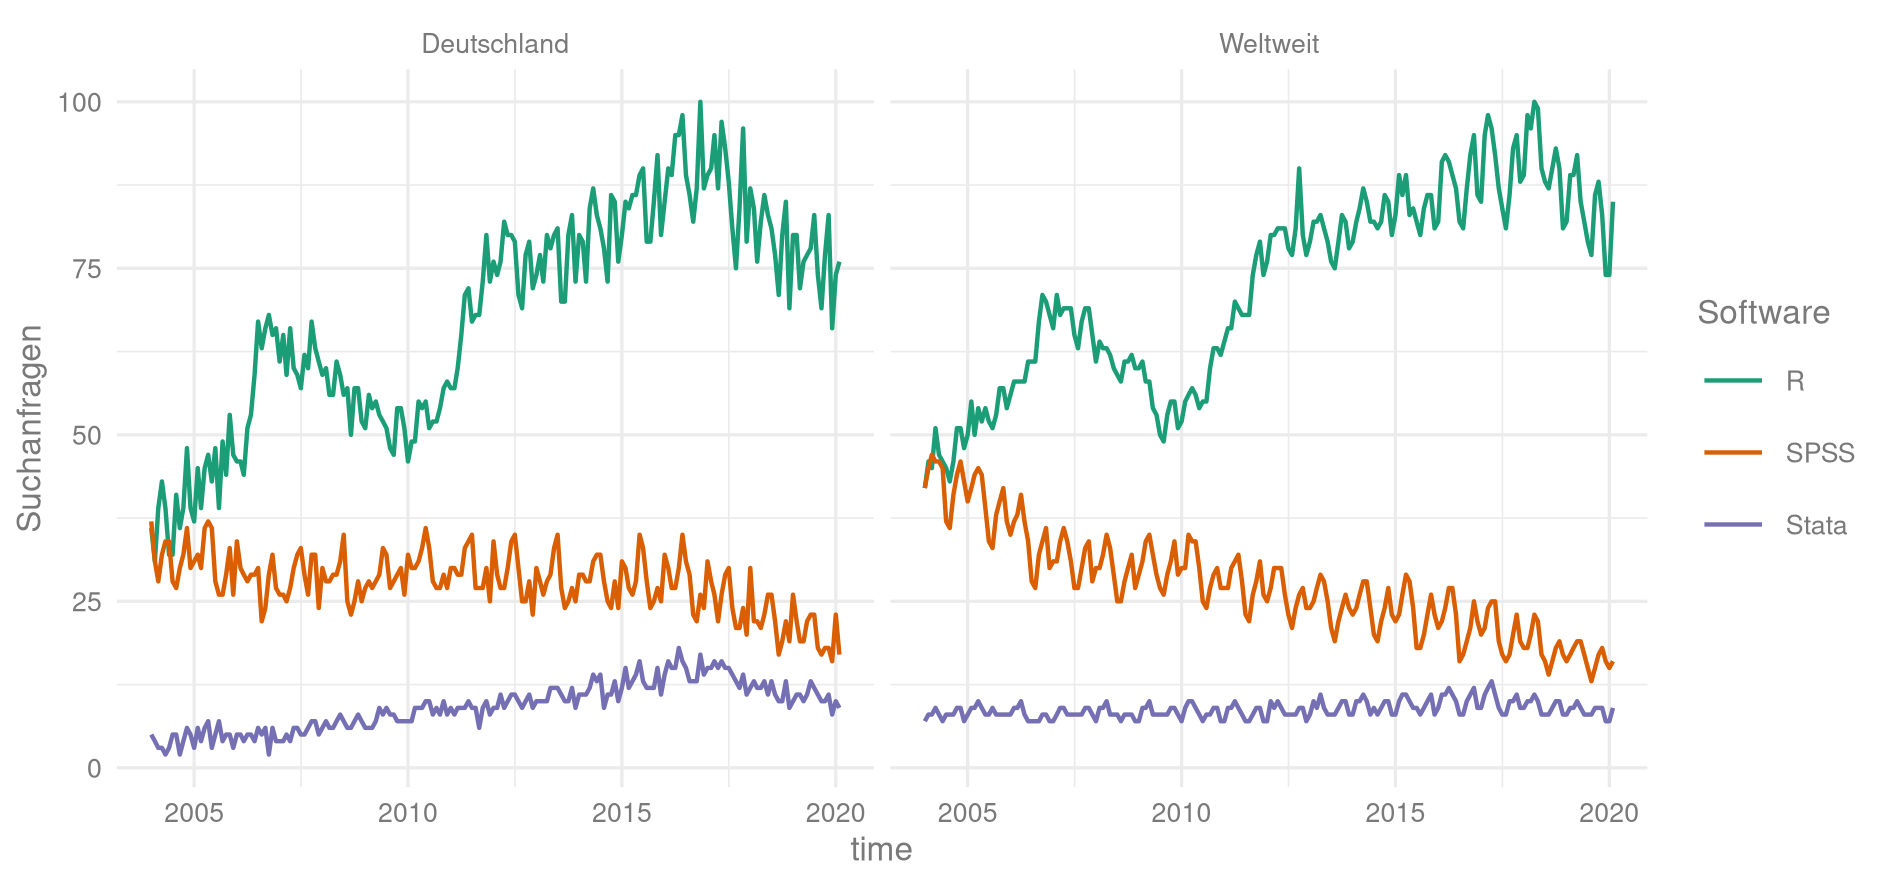
\includegraphics[width=333.333333333333pt]{imgs/gTrends} 

}

\caption{Google Suchanfragen, links aus [Deutschland](https://tinyurl.com/vosjrbz) und rechts [weltweit](https://tinyurl.com/vlwwp7a)}\label{fig:unnamed-chunk-3}
\end{figure}

\hypertarget{das-sind-nicht-alles-wissenschaftler}{%
\subsection{\ldots das sind nicht alles Wissenschaftler!}\label{das-sind-nicht-alles-wissenschaftler}}

\ldots stimmt, der Trend zeigt sich aber auch hier:

\begin{center}
\includegraphics[width=1\linewidth]{imgs/spss_1} \end{center}

\begin{center}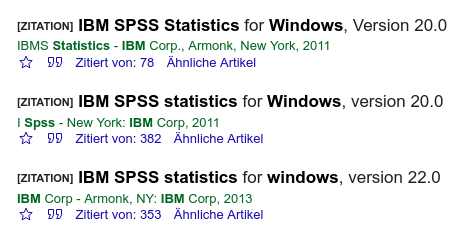
\includegraphics[width=1\linewidth]{imgs/spss_2} \end{center}

\begin{center}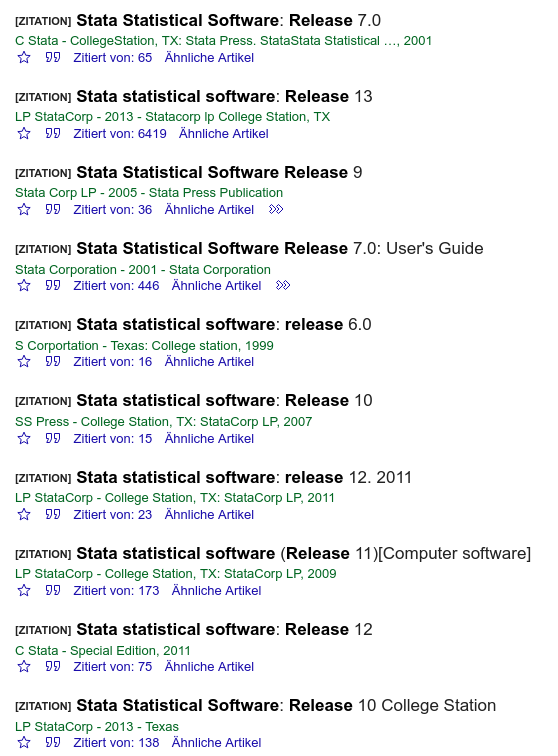
\includegraphics[width=1\linewidth]{imgs/Stata_1} \end{center}

\begin{center}
\includegraphics[width=1\linewidth]{imgs/R_1} \end{center}

\hypertarget{das-sind-doch-alles-nur-hilfeschreie}{%
\subsection{\ldots{} das sind doch alles nur Hilfeschreie!}\label{das-sind-doch-alles-nur-hilfeschreie}}

\ldots Möglich, aber dafür bekommt man für R auch leicht Hilfe.
Hier ein Beispiel von \href{https://stackoverflow.com}{stack overflow}:

\begin{center}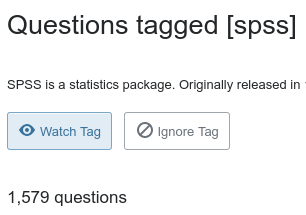
\includegraphics[width=0.8\linewidth]{imgs/so_spss} \end{center}

\begin{center}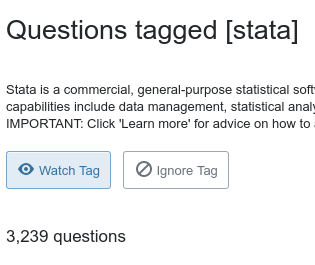
\includegraphics[width=0.8\linewidth]{imgs/so_stata} \end{center}

\begin{center}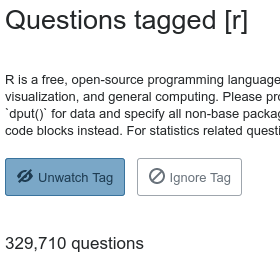
\includegraphics[width=0.8\linewidth]{imgs/so_r} \end{center}

\hypertarget{warum-r-1}{%
\subsection{Warum R?}\label{warum-r-1}}

\hypertarget{wir-fassen-zusammen}{%
\subsubsection{Wir fassen zusammen:}\label{wir-fassen-zusammen}}

R ist sehr beliebt und hat eine sehr aktive Community

\hypertarget{woran-liegt-das}{%
\subsubsection{Woran liegt das?}\label{woran-liegt-das}}

Das zentrale Argument:

\begin{itemize}
\tightlist
\item
  R ist Open Source und damit

  \begin{itemize}
  \tightlist
  \item
    kostenlos
  \item
    von der Community erweiterbar
  \end{itemize}
\end{itemize}

\hypertarget{warum-benutzen-wir-dann-nicht-alle-r}{%
\subsection{Warum benutzen wir dann nicht alle R?}\label{warum-benutzen-wir-dann-nicht-alle-r}}

\begin{quote}
\begin{itemize}
\tightlist
\item
  Mausnavigierte IDEs wirken erstmal intuitiver
\end{itemize}
\end{quote}

\begin{quote}
\begin{itemize}
\tightlist
\item
  Man braucht vor allem am Anfang (ein bisschen) Frustrationstoleranz
\end{itemize}
\end{quote}

\begin{quote}
\begin{itemize}
\tightlist
\item
  Die von der Community geschriebenen Erweiterungen (und über Strecken auch \texttt{base\ R}) haben keine einheitliche Syntax
\end{itemize}
\end{quote}

\hypertarget{aber}{%
\subsubsection{Aber:}\label{aber}}

\begin{itemize}
\item
  Man findet sehr schnell Hilfe
\item
  Es gibt Paketsammlungen, die einen Großteil der Datenaufbereitung und -analyse vereinheitlichen (z.B. das \texttt{tidyverse})
\end{itemize}

\hypertarget{r-syntax-basics}{%
\section{R-Syntax Basics}\label{r-syntax-basics}}

Die Absoluten Grundlagen der R Syntax sind:

\begin{enumerate}
\def\labelenumi{\arabic{enumi}.}
\item
  Zuweisungen und das \texttt{environment}
\item
  Funktionen und Argumente
\item
  Indizierung
\end{enumerate}

\hypertarget{zuweisungen-und-das-environment}{%
\subsection{1. Zuweisungen und das Environment}\label{zuweisungen-und-das-environment}}

Unter Zuweisung ist erstmal nichts anderes zu verstehen, als das Ablegen eines Zwischenergebnisses unter einem Namen, um es später weiterzuverwenden.

Auch wenn es andere Möglichkeiten gibt, ist die Folgende die lesbarste:

\begin{Shaded}
\begin{Highlighting}[]
\NormalTok{a\_number }\OtherTok{\textless{}{-}} \DecValTok{42}
\end{Highlighting}
\end{Shaded}

Die Zahl 42 ist jetzt für weitere Verwendung im \texttt{Environment} abgelegt:

\begin{center}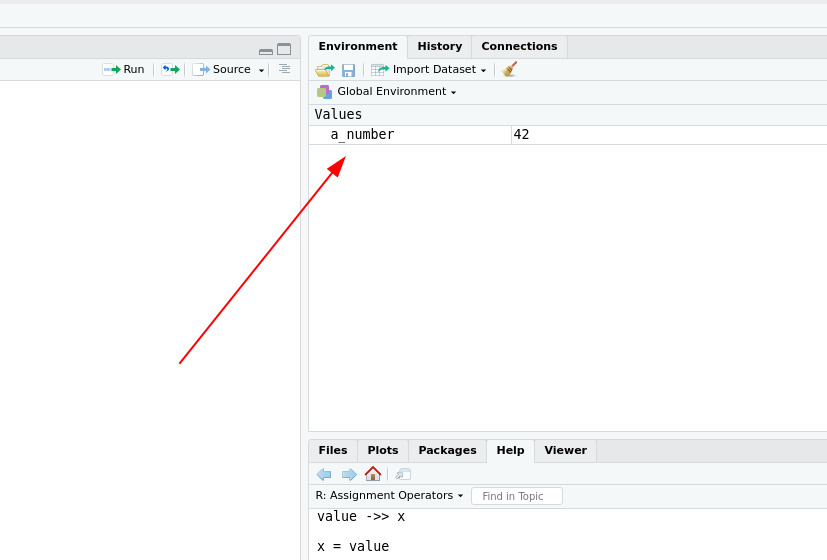
\includegraphics[width=0.6\linewidth]{imgs/environment} \end{center}

Und wie die Zahl alleine weiterzuverwenden:

\begin{Shaded}
\begin{Highlighting}[]
\DecValTok{42}\SpecialCharTok{\^{}}\DecValTok{2}
\end{Highlighting}
\end{Shaded}

\begin{verbatim}
## [1] 1764
\end{verbatim}

\begin{Shaded}
\begin{Highlighting}[]
\NormalTok{a\_number}\SpecialCharTok{\^{}}\DecValTok{2} \DocumentationTok{\#\# äquivalent}
\end{Highlighting}
\end{Shaded}

\begin{verbatim}
## [1] 1764
\end{verbatim}

Jede dieser in grau unterlegten Zeilen nennt man auch eine \emph{Anweisung}. R wird in der letzten Zeile angewiesen, den `Inhalt' von \texttt{a\_number} zu quadrieren. Dabei wird der dahinter durch das \texttt{\#}-Symbol eingeleitete Kommentar ignoriert.

\hypertarget{funktionen-und-argumente}{%
\subsection{2. Funktionen und Argumente}\label{funktionen-und-argumente}}

Der Großteil des in R erstellten Codes besteht aus \emph{Funktionen}.\\
Jede Funktion ist eine Sammlung an \emph{Anweisungen}, die nacheinander augeführt werden sollen.\\
\texttt{citation()} ist ein sehr einfaches Beispiel für eine solche Funktion.

Was macht \texttt{citation()}?

\texttt{citation()} gibt in der \emph{Konsole} aus, wie man R am Besten zitiert.

\begin{center}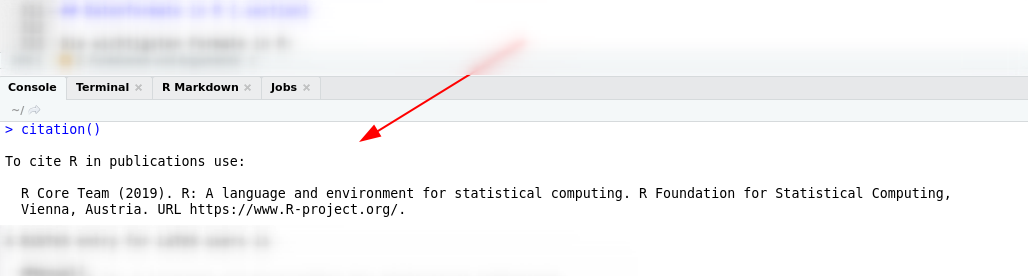
\includegraphics[width=0.8\linewidth]{imgs/citation} \end{center}

\hypertarget{obligatorische-und-optionale-argumente}{%
\subsection{2. obligatorische und optionale Argumente}\label{obligatorische-und-optionale-argumente}}

Die meisten Funktionen kommen aber nicht ohne \emph{Argumente} aus.\\
Argumente können in \emph{obligatorische} und \emph{optionale} unterteilt werden.

Wie die Namen schon sagen, sind \emph{obligatorische} Argumente solche, ohne die die Funktion nicht ausgeführt werden kann.\\
Obligatorische Argumente sind meistens die Werte, auf deren Basis gerade die Operationen ausgeführt werden sollen.

Wenn man keins oder ein falsches obligatorisches Argument übergibt, zeigt R einen Fehler an!

\emph{optionale} Argumente nennt man die, für die die Autoren der Funktion einen Standard vorgesehen haben. Das sind dann meist Stellschrauben, an denen das gewünschte Ergebnis genauer festgelegt werden kann. Werden diese Argumente nicht explizit gesetzt, wird einfach der Standard verwendet.

Ein Beispiel für eine Funktion, die obligatorische und optionale Argumente annimmt ist \texttt{round()}.

Auf der Hilfeseite von \texttt{round()} finden wir folgendes\footnote{Die Hilfeseite lässt sich entweder über die grafische Oberfläche oder mit \texttt{help(\textquotesingle{}round\textquotesingle{})} aufrufen.} :

\begin{center}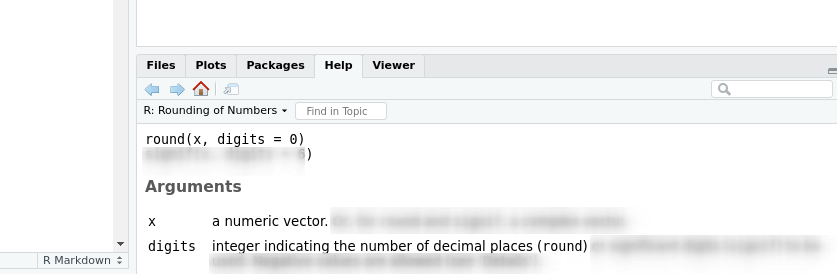
\includegraphics[width=0.8\linewidth]{imgs/help} \end{center}

Was ist hier das optionale Argument und wie erkennt man es?

\texttt{x} ist hier das obligatorische Argument (kein Standard durch ein \texttt{=}) angegeben

Wenn man \texttt{round} ohne ausprobiert, gibt es einen Fehler:

\begin{Shaded}
\begin{Highlighting}[]
\FunctionTok{round}\NormalTok{()}
\end{Highlighting}
\end{Shaded}

\begin{verbatim}
## Error in eval(expr, envir, enclos): 0 arguments passed to 'round' which requires 1 or 2 arguments
\end{verbatim}

Wen man eine Zahl übergibt, wird auf ganze Zahlen gerundet:

\begin{Shaded}
\begin{Highlighting}[]
\FunctionTok{round}\NormalTok{(}\FloatTok{3.1415}\NormalTok{)}
\end{Highlighting}
\end{Shaded}

\begin{verbatim}
## [1] 3
\end{verbatim}

Das optionale Argument \texttt{digits}, ermöglicht dann, die gewünschte Anzahl der Nachkommastellen anzugeben:

\begin{Shaded}
\begin{Highlighting}[]
\FunctionTok{round}\NormalTok{(}\FloatTok{3.1415}\NormalTok{, }\AttributeTok{digits =} \DecValTok{2}\NormalTok{)}
\end{Highlighting}
\end{Shaded}

\begin{verbatim}
## [1] 3.14
\end{verbatim}

Sowohl \texttt{3.1415} als auch \texttt{digits\ =\ 2} setzen Werte für Argumente!

Da die Funktion aber die zu rundende Zahl \texttt{x} an erster Stelle erwartet, ergibt der Aufruf das gewünschte Ergebnis.

\hypertarget{position-von-argumente}{%
\subsection{Position von Argumente}\label{position-von-argumente}}

R braucht also nicht unbedingt die Argumentnamen, wenn keine da sind wird die Reihenfolge interpretiert.

\begin{Shaded}
\begin{Highlighting}[]
\FunctionTok{round}\NormalTok{(}\FloatTok{3.1415}\NormalTok{, }\DecValTok{2}\NormalTok{) }\DocumentationTok{\#\# funktioniert, digits wird an zweiter Stelle erwartet}
\end{Highlighting}
\end{Shaded}

\begin{verbatim}
## [1] 3.14
\end{verbatim}

Was versucht R, wenn ich die folgende Anweisung ausführe?

\begin{Shaded}
\begin{Highlighting}[]
\FunctionTok{round}\NormalTok{(}\DecValTok{2}\NormalTok{, }\FloatTok{3.1415}\NormalTok{)}
\end{Highlighting}
\end{Shaded}

R rundet die Zahl 2 auf 3.1415 (also 3) Nachkommastellen.

\begin{Shaded}
\begin{Highlighting}[]
\FunctionTok{round}\NormalTok{(}\DecValTok{2}\NormalTok{, }\FloatTok{3.1415}\NormalTok{) }\DocumentationTok{\#\# funktioniert, aber vielleicht nicht wie erwartet}
\end{Highlighting}
\end{Shaded}

Wenn man Argumente ohne Namen in falscher Reihenfolge übergibt, gibt es keine Fehlermeldung aber Blödsinn!

\hypertarget{operatoren}{%
\subsection{Operatoren}\label{operatoren}}

Einzelne Zahlen benutzt man aber ja quasi nie. Deswegen hier eine sehr praktische Funktion:

\begin{Shaded}
\begin{Highlighting}[]
\DecValTok{1}\SpecialCharTok{:}\DecValTok{3}
\end{Highlighting}
\end{Shaded}

\begin{verbatim}
## [1] 1 2 3
\end{verbatim}

Huch! Das sieht ja gar nicht nach einer Funktion aus!

Neben den klassischen Funktionen, die durch ein Codewort und Klammern erkenntlich sind, gibt es in R noch eine Reihe \emph{Operatoren}, die auf den ersten Blick keine Funktionen sind.\\
Hier wird aber eigentlich `:`(1,3) ausgeführt, das Funktionsschema gilt also auch hier. `:`(1,3) ist nur schrecklich schlecht lesbar und viel zu viel zu tippen.

\hypertarget{indizierung}{%
\subsection{3. Indizierung}\label{indizierung}}

Da wir jetzt aber erste \texttt{Vektoren} mit mehr als einem Element erstellen können, gehen wir zu nächsten Part, der \emph{Indizierung} über.

In R lassen sich Elemente eines Objektes auf viele verschiedene Arten aufrufen, am Ende laufen diese aber auf den \texttt{{[}{]}}, den \texttt{{[}{[}{]}{]}} und den \texttt{\$}-Operator hinaus.

Für Vektoren reicht erstmal der \texttt{{[}{]}}-Operator.

Das einfachste Beispiel ist der Versuch, den 3. Wert aus einer Zahlenreihe ausgeben zu lassen.

Dafür erstellen wir zuerst die Zahlenreihe von 10 bis 15 und speichern diese im \texttt{Environment}

Wie mache ich das?

\begin{Shaded}
\begin{Highlighting}[]
\NormalTok{eine\_reihe\_von\_zahlen }\OtherTok{\textless{}{-}} \DecValTok{10}\SpecialCharTok{:}\DecValTok{15}
\end{Highlighting}
\end{Shaded}

Jetzt kann ich den \texttt{{[}{]}}-Operator benutzen, um den 3. Wert anzeigen zu lassen:

\begin{Shaded}
\begin{Highlighting}[]
\NormalTok{eine\_reihe\_von\_zahlen[}\DecValTok{3}\NormalTok{]}
\end{Highlighting}
\end{Shaded}

\begin{verbatim}
## [1] 12
\end{verbatim}

Und fertig. So einfach.

Der \texttt{{[}{]}}-Operator kann aber noch viel mehr. Ich kann zum Beispiel eine Sequenz übergeben, um eine Reihe von Zahlen ausgeben zu lassen:

\begin{Shaded}
\begin{Highlighting}[]
\NormalTok{eine\_reihe\_von\_zahlen[}\DecValTok{1}\SpecialCharTok{:}\DecValTok{3}\NormalTok{]}
\end{Highlighting}
\end{Shaded}

\begin{verbatim}
## [1] 10 11 12
\end{verbatim}

Der erste Wert ist die 10! der Index für die erste Stelle ist also die 1 (im Gegensatz zu Python z.B.)!

Eine weitere Möglichkeit ist die ausschließende Indizierung. Mit einem \texttt{-} gibt man an, dass einen alle außer der angegebenen Stelle interessieren.

\begin{Shaded}
\begin{Highlighting}[]
\NormalTok{eine\_reihe\_von\_zahlen[}\SpecialCharTok{{-}}\DecValTok{3}\NormalTok{]}
\end{Highlighting}
\end{Shaded}

\begin{verbatim}
## [1] 10 11 13 14 15
\end{verbatim}

\hypertarget{logische-indizierung}{%
\subsection{logische Indizierung}\label{logische-indizierung}}

Der \texttt{{[}{]}}-Operator kann außerdem benutzt werden, um über \emph{logische Operatoren} Werte zu indizieren.

Die einfachsten sind hier:

\begin{Shaded}
\begin{Highlighting}[]
\DecValTok{1} \SpecialCharTok{==} \DecValTok{2} \DocumentationTok{\#\# ist 1 gleich 2}
\DecValTok{1} \SpecialCharTok{!=} \DecValTok{3} \DocumentationTok{\#\# ist 1 ungleich 3}
\DecValTok{1} \SpecialCharTok{\textless{}} \DecValTok{4}  \DocumentationTok{\#\# ist 1 kleiner als 4}
\DecValTok{2} \SpecialCharTok{\textgreater{}=} \DecValTok{1} \DocumentationTok{\#\# ist 2 größer gleich 1}
\end{Highlighting}
\end{Shaded}

\begin{verbatim}
## [1] FALSE
## [1] TRUE
## [1] TRUE
## [1] TRUE
\end{verbatim}

Diese Operatoren kann ich auch auf Vektoren anwenden:

\begin{Shaded}
\begin{Highlighting}[]
\NormalTok{eine\_reihe\_von\_zahlen}\SpecialCharTok{\textgreater{}}\DecValTok{11}
\end{Highlighting}
\end{Shaded}

\begin{verbatim}
## [1] FALSE FALSE  TRUE  TRUE  TRUE  TRUE
\end{verbatim}

Und kann das Ergebnis auch mit dem \texttt{{[}{]}}-Operator kombinieren:

\begin{Shaded}
\begin{Highlighting}[]
\NormalTok{eine\_reihe\_von\_zahlen[eine\_reihe\_von\_zahlen}\SpecialCharTok{\textgreater{}}\DecValTok{11}\NormalTok{]}
\end{Highlighting}
\end{Shaded}

\begin{verbatim}
## [1] 12 13 14 15
\end{verbatim}

\hypertarget{datenformate-in-r}{%
\section{Datenformate in R}\label{datenformate-in-r}}

Bei der letzten Operation haben wir zwei Datenformate kennengelernt:

\begin{itemize}
\item
  \texttt{logical}, eine binär-logische Angabe und
\item
  \texttt{numeric}, alle ganze und (darstellbare) rationale Zahlen
\end{itemize}

Jetzt kennen wir schon 2 der 3 wichtigsten einfachen oder \texttt{atomic} Datenformate in R

Neben Zahlen muss R aber natürlich auch Text verarbeiten können. Dies geschieht über das \texttt{character}-Datenformat.

Wie könnte ich versuchen, ein \texttt{character}-Objekt mit dem Inhalt ``Ich bin ein String'' anzulegen?

\begin{Shaded}
\begin{Highlighting}[]
\NormalTok{ein\_toller\_character }\OtherTok{\textless{}{-}} \StringTok{"Ich bin ein String"}
\end{Highlighting}
\end{Shaded}

Diese einfachen Datenformate haben eine Hierarchie, die man so darzustellen versuchen könnte:

logical \textless{} numeric \textless{} character

Um uns das zu verdeutlichen, lernen wir noch eine neue Funktion:

\begin{itemize}
\tightlist
\item
  \texttt{c()} - die Vektor-Funktion. Mit ihr können wir Vektoren erstellen und Werte zu bestehenden Vektoren hinzufügen.
\end{itemize}

\begin{Shaded}
\begin{Highlighting}[]
\NormalTok{logical\_vector }\OtherTok{\textless{}{-}} \FunctionTok{c}\NormalTok{(}\ConstantTok{TRUE}\NormalTok{, }\ConstantTok{TRUE}\NormalTok{, }\ConstantTok{FALSE}\NormalTok{)}
\NormalTok{logical\_vector}
\end{Highlighting}
\end{Shaded}

\begin{verbatim}
## [1]  TRUE  TRUE FALSE
\end{verbatim}

\begin{Shaded}
\begin{Highlighting}[]
\FunctionTok{c}\NormalTok{(logical\_vector,}\DecValTok{1}\NormalTok{)}
\end{Highlighting}
\end{Shaded}

\begin{verbatim}
## [1] 1 1 0 1
\end{verbatim}

Die logischen Werte wurden in Zahlen umgewandelt.

Was passiert wohl, wenn wir eine 1 \emph{und} einen \texttt{character} hinzufügen?

\begin{Shaded}
\begin{Highlighting}[]
\FunctionTok{c}\NormalTok{(logical\_vector,}\DecValTok{1}\NormalTok{,}\StringTok{\textquotesingle{}ein character\textquotesingle{}}\NormalTok{)}
\end{Highlighting}
\end{Shaded}

\begin{verbatim}
## [1] "TRUE"          "TRUE"         
## [3] "FALSE"         "1"            
## [5] "ein character"
\end{verbatim}

Die logischen Werte und die Zahl wurden in \texttt{character} umgewandelt

Die \texttt{atomics} haben eine klare Hierarchie!

Rückgängig machen lässt sich das durch \texttt{as.logical}, \texttt{as.numeric} und \texttt{as.character}. Aber Vorsicht, so können auch leicht fehlende Werte, durch \texttt{NA} gekennzeichnet erzeugt werden:

\begin{Shaded}
\begin{Highlighting}[]
\NormalTok{ein\_umzuwandelnder\_vektor }\OtherTok{\textless{}{-}} \FunctionTok{c}\NormalTok{(}\StringTok{\textquotesingle{}a\textquotesingle{}}\NormalTok{,}\DecValTok{1}\NormalTok{,}\DecValTok{15}\NormalTok{,}\ConstantTok{TRUE}\NormalTok{)}
\FunctionTok{as.numeric}\NormalTok{(ein\_umzuwandelnder\_vektor)}
\end{Highlighting}
\end{Shaded}

\begin{verbatim}
## Warning: NAs introduced by coercion
\end{verbatim}

\begin{verbatim}
## [1] NA  1 15 NA
\end{verbatim}

\begin{Shaded}
\begin{Highlighting}[]
\FunctionTok{as.numeric}\NormalTok{(ein\_umzuwandelnder\_vektor)}
\end{Highlighting}
\end{Shaded}

\begin{verbatim}
## Warning: NAs introduced by coercion
\end{verbatim}

\begin{verbatim}
## [1] NA  1 15 NA
\end{verbatim}

Warum fehlt auch der letzte Wert?

Weil das \texttt{TRUE} inzwischen ein \texttt{character} ist.

\begin{Shaded}
\begin{Highlighting}[]
\NormalTok{ein\_umzuwandelnder\_vektor}
\end{Highlighting}
\end{Shaded}

\begin{verbatim}
## [1] "a"    "1"    "15"   "TRUE"
\end{verbatim}

Natürlich gibt es auch komplexere, mehrsimensionale Datenformate in R, um die kümmern wir uns dann nach der Pause.

\hypertarget{daten-manipulieren}{%
\chapter{Daten manipulieren}\label{daten-manipulieren}}

\hypertarget{datensuxe4tze-in-r}{%
\section{Datensätze in R}\label{datensuxe4tze-in-r}}

Wie alle anderen Programme zur statistischen Auswertung hat R natürlich neben den Vektoren auch rechteckige Datenformate.

Das typische rechteckige Datenformat in \texttt{base\ R} ist der \texttt{data.frame}. Im Prinzip nichts anderes, als spaltenweise zusammengeklebte Vektoren.
Der Konstruktor für ein solches Objekt heißt ist die gleichnamige Funktion, die die Spalten als benannte Argumente nimmt:

\begin{Shaded}
\begin{Highlighting}[]
\NormalTok{df }\OtherTok{\textless{}{-}} \FunctionTok{data.frame}\NormalTok{(}\AttributeTok{a =} \DecValTok{1}\SpecialCharTok{:}\DecValTok{3}\NormalTok{,}
                 \AttributeTok{b =} \FunctionTok{c}\NormalTok{(}\ConstantTok{TRUE}\NormalTok{, }\ConstantTok{FALSE}\NormalTok{, }\ConstantTok{TRUE}\NormalTok{),}
                 \AttributeTok{c =} \FunctionTok{c}\NormalTok{(}\StringTok{\textquotesingle{}a\textquotesingle{}}\NormalTok{,}\StringTok{\textquotesingle{}b\textquotesingle{}}\NormalTok{,}\StringTok{\textquotesingle{}c\textquotesingle{}}\NormalTok{))}
\NormalTok{df}
\end{Highlighting}
\end{Shaded}

\begin{verbatim}
##   a     b c
## 1 1  TRUE a
## 2 2 FALSE b
## 3 3  TRUE c
\end{verbatim}

Das Indizieren im Datensatz geht dann am \emph{Lesbarsten}, durch das Angeben der gewünschten Spalte mit dem \texttt{\$}-Operator und der Auswahl der Zeile durch den schon bekannten \texttt{{[}{]}}-Operator.

\begin{Shaded}
\begin{Highlighting}[]
\NormalTok{df}\SpecialCharTok{$}\NormalTok{c[}\DecValTok{2}\NormalTok{] }\DocumentationTok{\#\# 2. Wert in der \textquotesingle{}c\textquotesingle{}{-}Spalte.}
\end{Highlighting}
\end{Shaded}

\begin{verbatim}
## [1] "b"
\end{verbatim}

Wie könnte ich den 3. Wert in der \texttt{b}-Spalte indizieren?

\texttt{df\$b{[}3{]}}

Der \texttt{iris}-Datensatz ist ein im Grundumfang von R mitgelieferter Datensatz, der historische botanische Daten nach \citet{andersonIrisesGaspePeninsula1935} enthält.

\begin{Shaded}
\begin{Highlighting}[]
\NormalTok{iris}
\end{Highlighting}
\end{Shaded}

\begin{verbatim}
##     Sepal.Length Sepal.Width Petal.Length
## 1            5.1         3.5          1.4
## 2            4.9         3.0          1.4
## 3            4.7         3.2          1.3
## 4            4.6         3.1          1.5
## 5            5.0         3.6          1.4
## 6            5.4         3.9          1.7
## 7            4.6         3.4          1.4
## 8            5.0         3.4          1.5
## 9            4.4         2.9          1.4
## 10           4.9         3.1          1.5
## 11           5.4         3.7          1.5
## 12           4.8         3.4          1.6
## 13           4.8         3.0          1.4
## 14           4.3         3.0          1.1
## 15           5.8         4.0          1.2
## 16           5.7         4.4          1.5
## 17           5.4         3.9          1.3
## 18           5.1         3.5          1.4
## 19           5.7         3.8          1.7
## 20           5.1         3.8          1.5
## 21           5.4         3.4          1.7
## 22           5.1         3.7          1.5
## 23           4.6         3.6          1.0
## 24           5.1         3.3          1.7
## 25           4.8         3.4          1.9
## 26           5.0         3.0          1.6
## 27           5.0         3.4          1.6
## 28           5.2         3.5          1.5
## 29           5.2         3.4          1.4
## 30           4.7         3.2          1.6
## 31           4.8         3.1          1.6
## 32           5.4         3.4          1.5
## 33           5.2         4.1          1.5
## 34           5.5         4.2          1.4
## 35           4.9         3.1          1.5
## 36           5.0         3.2          1.2
## 37           5.5         3.5          1.3
## 38           4.9         3.6          1.4
## 39           4.4         3.0          1.3
## 40           5.1         3.4          1.5
## 41           5.0         3.5          1.3
## 42           4.5         2.3          1.3
## 43           4.4         3.2          1.3
## 44           5.0         3.5          1.6
## 45           5.1         3.8          1.9
## 46           4.8         3.0          1.4
## 47           5.1         3.8          1.6
## 48           4.6         3.2          1.4
## 49           5.3         3.7          1.5
## 50           5.0         3.3          1.4
## 51           7.0         3.2          4.7
## 52           6.4         3.2          4.5
## 53           6.9         3.1          4.9
## 54           5.5         2.3          4.0
## 55           6.5         2.8          4.6
## 56           5.7         2.8          4.5
## 57           6.3         3.3          4.7
## 58           4.9         2.4          3.3
## 59           6.6         2.9          4.6
## 60           5.2         2.7          3.9
## 61           5.0         2.0          3.5
## 62           5.9         3.0          4.2
## 63           6.0         2.2          4.0
## 64           6.1         2.9          4.7
## 65           5.6         2.9          3.6
## 66           6.7         3.1          4.4
## 67           5.6         3.0          4.5
## 68           5.8         2.7          4.1
## 69           6.2         2.2          4.5
## 70           5.6         2.5          3.9
## 71           5.9         3.2          4.8
## 72           6.1         2.8          4.0
## 73           6.3         2.5          4.9
## 74           6.1         2.8          4.7
## 75           6.4         2.9          4.3
## 76           6.6         3.0          4.4
## 77           6.8         2.8          4.8
## 78           6.7         3.0          5.0
## 79           6.0         2.9          4.5
## 80           5.7         2.6          3.5
## 81           5.5         2.4          3.8
## 82           5.5         2.4          3.7
## 83           5.8         2.7          3.9
## 84           6.0         2.7          5.1
## 85           5.4         3.0          4.5
## 86           6.0         3.4          4.5
## 87           6.7         3.1          4.7
## 88           6.3         2.3          4.4
## 89           5.6         3.0          4.1
## 90           5.5         2.5          4.0
## 91           5.5         2.6          4.4
## 92           6.1         3.0          4.6
## 93           5.8         2.6          4.0
## 94           5.0         2.3          3.3
## 95           5.6         2.7          4.2
## 96           5.7         3.0          4.2
## 97           5.7         2.9          4.2
## 98           6.2         2.9          4.3
## 99           5.1         2.5          3.0
## 100          5.7         2.8          4.1
## 101          6.3         3.3          6.0
## 102          5.8         2.7          5.1
## 103          7.1         3.0          5.9
## 104          6.3         2.9          5.6
## 105          6.5         3.0          5.8
## 106          7.6         3.0          6.6
## 107          4.9         2.5          4.5
## 108          7.3         2.9          6.3
## 109          6.7         2.5          5.8
## 110          7.2         3.6          6.1
## 111          6.5         3.2          5.1
## 112          6.4         2.7          5.3
## 113          6.8         3.0          5.5
## 114          5.7         2.5          5.0
## 115          5.8         2.8          5.1
## 116          6.4         3.2          5.3
## 117          6.5         3.0          5.5
## 118          7.7         3.8          6.7
## 119          7.7         2.6          6.9
## 120          6.0         2.2          5.0
## 121          6.9         3.2          5.7
## 122          5.6         2.8          4.9
## 123          7.7         2.8          6.7
## 124          6.3         2.7          4.9
## 125          6.7         3.3          5.7
## 126          7.2         3.2          6.0
## 127          6.2         2.8          4.8
## 128          6.1         3.0          4.9
## 129          6.4         2.8          5.6
## 130          7.2         3.0          5.8
## 131          7.4         2.8          6.1
## 132          7.9         3.8          6.4
## 133          6.4         2.8          5.6
## 134          6.3         2.8          5.1
## 135          6.1         2.6          5.6
## 136          7.7         3.0          6.1
## 137          6.3         3.4          5.6
## 138          6.4         3.1          5.5
## 139          6.0         3.0          4.8
## 140          6.9         3.1          5.4
## 141          6.7         3.1          5.6
## 142          6.9         3.1          5.1
## 143          5.8         2.7          5.1
## 144          6.8         3.2          5.9
## 145          6.7         3.3          5.7
## 146          6.7         3.0          5.2
## 147          6.3         2.5          5.0
## 148          6.5         3.0          5.2
## 149          6.2         3.4          5.4
## 150          5.9         3.0          5.1
##     Petal.Width    Species
## 1           0.2     setosa
## 2           0.2     setosa
## 3           0.2     setosa
## 4           0.2     setosa
## 5           0.2     setosa
## 6           0.4     setosa
## 7           0.3     setosa
## 8           0.2     setosa
## 9           0.2     setosa
## 10          0.1     setosa
## 11          0.2     setosa
## 12          0.2     setosa
## 13          0.1     setosa
## 14          0.1     setosa
## 15          0.2     setosa
## 16          0.4     setosa
## 17          0.4     setosa
## 18          0.3     setosa
## 19          0.3     setosa
## 20          0.3     setosa
## 21          0.2     setosa
## 22          0.4     setosa
## 23          0.2     setosa
## 24          0.5     setosa
## 25          0.2     setosa
## 26          0.2     setosa
## 27          0.4     setosa
## 28          0.2     setosa
## 29          0.2     setosa
## 30          0.2     setosa
## 31          0.2     setosa
## 32          0.4     setosa
## 33          0.1     setosa
## 34          0.2     setosa
## 35          0.2     setosa
## 36          0.2     setosa
## 37          0.2     setosa
## 38          0.1     setosa
## 39          0.2     setosa
## 40          0.2     setosa
## 41          0.3     setosa
## 42          0.3     setosa
## 43          0.2     setosa
## 44          0.6     setosa
## 45          0.4     setosa
## 46          0.3     setosa
## 47          0.2     setosa
## 48          0.2     setosa
## 49          0.2     setosa
## 50          0.2     setosa
## 51          1.4 versicolor
## 52          1.5 versicolor
## 53          1.5 versicolor
## 54          1.3 versicolor
## 55          1.5 versicolor
## 56          1.3 versicolor
## 57          1.6 versicolor
## 58          1.0 versicolor
## 59          1.3 versicolor
## 60          1.4 versicolor
## 61          1.0 versicolor
## 62          1.5 versicolor
## 63          1.0 versicolor
## 64          1.4 versicolor
## 65          1.3 versicolor
## 66          1.4 versicolor
## 67          1.5 versicolor
## 68          1.0 versicolor
## 69          1.5 versicolor
## 70          1.1 versicolor
## 71          1.8 versicolor
## 72          1.3 versicolor
## 73          1.5 versicolor
## 74          1.2 versicolor
## 75          1.3 versicolor
## 76          1.4 versicolor
## 77          1.4 versicolor
## 78          1.7 versicolor
## 79          1.5 versicolor
## 80          1.0 versicolor
## 81          1.1 versicolor
## 82          1.0 versicolor
## 83          1.2 versicolor
## 84          1.6 versicolor
## 85          1.5 versicolor
## 86          1.6 versicolor
## 87          1.5 versicolor
## 88          1.3 versicolor
## 89          1.3 versicolor
## 90          1.3 versicolor
## 91          1.2 versicolor
## 92          1.4 versicolor
## 93          1.2 versicolor
## 94          1.0 versicolor
## 95          1.3 versicolor
## 96          1.2 versicolor
## 97          1.3 versicolor
## 98          1.3 versicolor
## 99          1.1 versicolor
## 100         1.3 versicolor
## 101         2.5  virginica
## 102         1.9  virginica
## 103         2.1  virginica
## 104         1.8  virginica
## 105         2.2  virginica
## 106         2.1  virginica
## 107         1.7  virginica
## 108         1.8  virginica
## 109         1.8  virginica
## 110         2.5  virginica
## 111         2.0  virginica
## 112         1.9  virginica
## 113         2.1  virginica
## 114         2.0  virginica
## 115         2.4  virginica
## 116         2.3  virginica
## 117         1.8  virginica
## 118         2.2  virginica
## 119         2.3  virginica
## 120         1.5  virginica
## 121         2.3  virginica
## 122         2.0  virginica
## 123         2.0  virginica
## 124         1.8  virginica
## 125         2.1  virginica
## 126         1.8  virginica
## 127         1.8  virginica
## 128         1.8  virginica
## 129         2.1  virginica
## 130         1.6  virginica
## 131         1.9  virginica
## 132         2.0  virginica
## 133         2.2  virginica
## 134         1.5  virginica
## 135         1.4  virginica
## 136         2.3  virginica
## 137         2.4  virginica
## 138         1.8  virginica
## 139         1.8  virginica
## 140         2.1  virginica
## 141         2.4  virginica
## 142         2.3  virginica
## 143         1.9  virginica
## 144         2.3  virginica
## 145         2.5  virginica
## 146         2.3  virginica
## 147         1.9  virginica
## 148         2.0  virginica
## 149         2.3  virginica
## 150         1.8  virginica
\end{verbatim}

\hypertarget{uxfcbersicht-uxfcber-datensatz-verschaffen}{%
\subsection{Übersicht über Datensatz verschaffen}\label{uxfcbersicht-uxfcber-datensatz-verschaffen}}

Das ist natürlich ein bisschen unübersichtlich, wie kann man damit umgehen?

\hypertarget{muxf6glichkeit}{%
\subsubsection{1. Möglichkeit:}\label{muxf6glichkeit}}

Wenn man iris explizit in das Environment nimmt, kann man die Oberfläche von RStudio nutze, um sich einen Überblick zu verschaffen\footnote{Dabei nutzt die RStudio-IDE aber nur die \texttt{str()}(für structure)-Funktion.}:

\begin{Shaded}
\begin{Highlighting}[]
\NormalTok{iris }\OtherTok{\textless{}{-}}\NormalTok{ iris}
\end{Highlighting}
\end{Shaded}

\begin{center}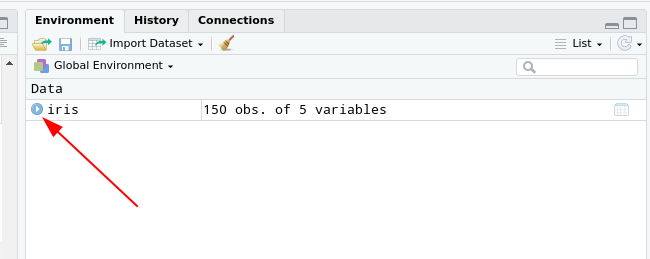
\includegraphics[width=1\linewidth]{imgs/summ1} \end{center}

\begin{center}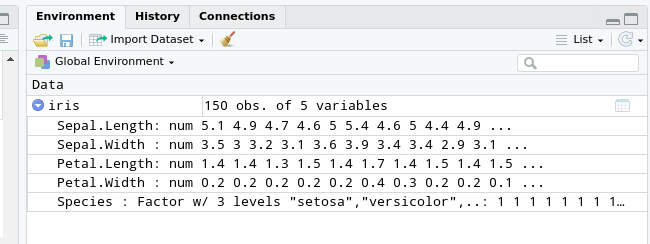
\includegraphics[width=1\linewidth]{imgs/summ2} \end{center}

\hypertarget{muxf6glichkeit-1}{%
\subsubsection{2. Möglichkeit:}\label{muxf6glichkeit-1}}

Die \texttt{summary}-Funktion, die genau das macht, was ihr Name suggeriert:

\begin{Shaded}
\begin{Highlighting}[]
\FunctionTok{summary}\NormalTok{(iris)}
\end{Highlighting}
\end{Shaded}

\begin{verbatim}
##   Sepal.Length    Sepal.Width     Petal.Length  
##  Min.   :4.300   Min.   :2.000   Min.   :1.000  
##  1st Qu.:5.100   1st Qu.:2.800   1st Qu.:1.600  
##  Median :5.800   Median :3.000   Median :4.350  
##  Mean   :5.843   Mean   :3.057   Mean   :3.758  
##  3rd Qu.:6.400   3rd Qu.:3.300   3rd Qu.:5.100  
##  Max.   :7.900   Max.   :4.400   Max.   :6.900  
##   Petal.Width          Species  
##  Min.   :0.100   setosa    :50  
##  1st Qu.:0.300   versicolor:50  
##  Median :1.300   virginica :50  
##  Mean   :1.199                  
##  3rd Qu.:1.800                  
##  Max.   :2.500
\end{verbatim}

\hypertarget{aufgabe-deskriptive-kennwerte-berechnen}{%
\subsection{Aufgabe: Deskriptive Kennwerte berechnen}\label{aufgabe-deskriptive-kennwerte-berechnen}}

Wir wollen für diesen Datensatz jetzt die folgenden Schritte der Auswertung vollziehen:

\begin{enumerate}
\def\labelenumi{\arabic{enumi}.}
\item
  Ausschluss der Blumen, die breitere Blütenblätter als das 1.5-fache der mittleren Blütenblätter haben und Kelche, die kürzer als das Mittel der Kelchlänge sind
\item
  Darstellung der Mittelwerte und Streuungen der Blütenblattlänge und -breite pro verbleibende Spezies als Tabelle
\end{enumerate}

\hypertarget{aufgabe-base-r-luxf6sung}{%
\subsection{Aufgabe: Base-R Lösung}\label{aufgabe-base-r-luxf6sung}}

\begin{Shaded}
\begin{Highlighting}[]
\NormalTok{df }\OtherTok{\textless{}{-}}\NormalTok{ iris[iris}\SpecialCharTok{$}\NormalTok{Petal.Width }\SpecialCharTok{\textless{}=} \FloatTok{1.5} \SpecialCharTok{*} \FunctionTok{mean}\NormalTok{(iris}\SpecialCharTok{$}\NormalTok{Petal.Width) }\SpecialCharTok{\&}
\NormalTok{             iris}\SpecialCharTok{$}\NormalTok{Sepal.Length }\SpecialCharTok{\textgreater{}=} \FunctionTok{mean}\NormalTok{(iris}\SpecialCharTok{$}\NormalTok{Sepal.Length),]}
\NormalTok{means }\OtherTok{\textless{}{-}} \FunctionTok{aggregate}\NormalTok{(}\FunctionTok{cbind}\NormalTok{(df}\SpecialCharTok{$}\NormalTok{Petal.Length,df}\SpecialCharTok{$}\NormalTok{Petal.Width),}
          \AttributeTok{by =} \FunctionTok{list}\NormalTok{(}\AttributeTok{Species =}\NormalTok{ df}\SpecialCharTok{$}\NormalTok{Species),}
          \AttributeTok{FUN =}\NormalTok{ mean)}
\NormalTok{sds }\OtherTok{\textless{}{-}} \FunctionTok{aggregate}\NormalTok{(}\FunctionTok{cbind}\NormalTok{(df}\SpecialCharTok{$}\NormalTok{Petal.Length,df}\SpecialCharTok{$}\NormalTok{Petal.Width),}
          \AttributeTok{by =} \FunctionTok{list}\NormalTok{(}\AttributeTok{Species =}\NormalTok{ df}\SpecialCharTok{$}\NormalTok{Species),}
          \AttributeTok{FUN =}\NormalTok{ sd)}
\NormalTok{tab }\OtherTok{\textless{}{-}} \FunctionTok{data.frame}\NormalTok{(means, sds[,}\DecValTok{2}\SpecialCharTok{:}\DecValTok{3}\NormalTok{])}
\FunctionTok{names}\NormalTok{(tab)[}\DecValTok{2}\SpecialCharTok{:}\DecValTok{5}\NormalTok{] }\OtherTok{=} \FunctionTok{c}\NormalTok{(}\StringTok{\textquotesingle{}m\_Length\textquotesingle{}}\NormalTok{, }\StringTok{\textquotesingle{}m\_Width\textquotesingle{}}\NormalTok{, }\StringTok{\textquotesingle{}sd\_Length\textquotesingle{}}\NormalTok{, }\StringTok{\textquotesingle{}sd\_Width\textquotesingle{}}\NormalTok{)}
\NormalTok{tab}
\end{Highlighting}
\end{Shaded}

\begin{verbatim}
##      Species m_Length m_Width sd_Length
## 1 versicolor    4.560   1.424 0.2783882
## 2  virginica    5.375   1.500 0.3862210
##     sd_Width
## 1 0.14798649
## 2 0.08164966
\end{verbatim}

\hypertarget{auftritt-tidyverse}{%
\subsection{Auftritt tidyverse}\label{auftritt-tidyverse}}

Die selbe Aufgabe wie gerade, jetzt mit dem \texttt{tidyverse}:

\begin{Shaded}
\begin{Highlighting}[]
\FunctionTok{library}\NormalTok{(tidyverse)}
\NormalTok{iris }\SpecialCharTok{\%\textgreater{}\%} 
  \FunctionTok{filter}\NormalTok{(Petal.Width }\SpecialCharTok{\textless{}=} \FloatTok{1.5} \SpecialCharTok{*} \FunctionTok{mean}\NormalTok{(Petal.Width) }\SpecialCharTok{\&}
\NormalTok{           Sepal.Length }\SpecialCharTok{\textgreater{}=} \FunctionTok{mean}\NormalTok{(Sepal.Length)) }\SpecialCharTok{\%\textgreater{}\%} 
  \FunctionTok{group\_by}\NormalTok{(Species) }\SpecialCharTok{\%\textgreater{}\%} 
  \FunctionTok{summarise}\NormalTok{(}\AttributeTok{m\_Length =} \FunctionTok{mean}\NormalTok{(Petal.Length),}
            \AttributeTok{sd\_Length =} \FunctionTok{sd}\NormalTok{(Petal.Length),}
            \AttributeTok{m\_Width =} \FunctionTok{mean}\NormalTok{(Petal.Width), }
            \AttributeTok{sd\_Width =} \FunctionTok{sd}\NormalTok{(Petal.Width))}
\end{Highlighting}
\end{Shaded}

\begin{verbatim}
## `summarise()` ungrouping output (override with `.groups` argument)
\end{verbatim}

\begin{verbatim}
## # A tibble: 2 x 5
##   Species    m_Length sd_Length m_Width sd_Width
##   <fct>         <dbl>     <dbl>   <dbl>    <dbl>
## 1 versicolor     4.56     0.278    1.42   0.148 
## 2 virginica      5.38     0.386    1.5    0.0816
\end{verbatim}

\hypertarget{tidy-aggregation}{%
\subsection{tidy aggregation}\label{tidy-aggregation}}

Das \texttt{tidyverse} ist eine Sammlung von Paketen, deren Hauptziel es ist, Datenaufbereitung in R intuitiver und leichter lesbar zu machen.

Ein zentrales Element dabei ist der \texttt{\%\textgreater{}\%}-Operator, die sogenannte Pipeline. Beim Skript-Lesen und -Schreiben kann man sich diese am Besten als \emph{`dann'} vorstellen

Mit ihrer Hilfe werden Aufbereitungsschritte in einer stringenten Reihe an Operationen formuliert, die sich am Besten als Satz verstehen lassen.

Da die Funktionen im tidyverse alle mit einfachen Verben benannt sind, lässt sich die Operation von eben auch so lesen.

\begin{Shaded}
\begin{Highlighting}[]
\NormalTok{iris }\SpecialCharTok{\%\textgreater{}\%} 
\end{Highlighting}
\end{Shaded}

Nimm \texttt{iris}, dann \ldots{}

\begin{Shaded}
\begin{Highlighting}[]
  \FunctionTok{filter}\NormalTok{(Petal.Width }\SpecialCharTok{\textless{}=} \FloatTok{1.5} \SpecialCharTok{*} \FunctionTok{mean}\NormalTok{(Petal.Width) }\SpecialCharTok{\&}
\NormalTok{           Sepal.Length }\SpecialCharTok{\textgreater{}=} \FunctionTok{mean}\NormalTok{(Sepal.Length)) }\SpecialCharTok{\%\textgreater{}\%} 
\end{Highlighting}
\end{Shaded}

\ldots{} filter Zeilenweise nach den gesetzten Regeln, dann\ldots{}

\begin{Shaded}
\begin{Highlighting}[]
  \FunctionTok{group\_by}\NormalTok{(Species) }\SpecialCharTok{\%\textgreater{}\%} 
\end{Highlighting}
\end{Shaded}

\ldots gruppiere nach der Spezies, dann\ldots{}

\begin{Shaded}
\begin{Highlighting}[]
  \FunctionTok{summarise}\NormalTok{(}\AttributeTok{m\_Length =} \FunctionTok{mean}\NormalTok{(Petal.Length),}
            \AttributeTok{sd\_Length =} \FunctionTok{sd}\NormalTok{(Petal.Length),}
            \AttributeTok{m\_Width =} \FunctionTok{mean}\NormalTok{(Petal.Width), }
            \AttributeTok{sd\_Width =} \FunctionTok{sd}\NormalTok{(Petal.Width))}
\end{Highlighting}
\end{Shaded}

\ldots{} berechne die angegebenen Kenngrößen über die Gruppen.

Zweite Beispielaufgabe:

Wir möchten für den \texttt{iris}-Datensatz:

\begin{enumerate}
\def\labelenumi{\arabic{enumi}.}
\item
  Eine Spalte hinzufügen, die die z-transformierte Blattlänge enthält
\item
  Eine Spalte hinzufügen, die als character das Ergebnis eines Mediansplits der gerade erstellten Variable enthält
\item
  Einen Datensatz erstellen, der nur die Spezies, die z-Transformierte und die Mediansplit-Variable enthält
\item
  Die Häufigkeiten der Kombinationen von Mediansplit-Gruppe und Spezies auszählen
\end{enumerate}

\begin{Shaded}
\begin{Highlighting}[]
\NormalTok{df }\OtherTok{\textless{}{-}}\NormalTok{ iris }\SpecialCharTok{\%\textgreater{}\%} 
  \FunctionTok{mutate}\NormalTok{(}\AttributeTok{z\_length =}\NormalTok{ (Petal.Length}\SpecialCharTok{{-}}\FunctionTok{mean}\NormalTok{(Petal.Length))}\SpecialCharTok{/}\FunctionTok{sd}\NormalTok{(Petal.Length),}
        \AttributeTok{med\_split =} \FunctionTok{ifelse}\NormalTok{(z\_length }\SpecialCharTok{\textgreater{}=} \FunctionTok{median}\NormalTok{(z\_length),}
                            \StringTok{\textquotesingle{}upper\textquotesingle{}}\NormalTok{,}
                            \StringTok{\textquotesingle{}lower\textquotesingle{}}\NormalTok{)) }\SpecialCharTok{\%\textgreater{}\%} 
  \FunctionTok{select}\NormalTok{(Species, z\_length, med\_split) }
\end{Highlighting}
\end{Shaded}

Hat das geklappt?

Wie könnte ich das überprüfen?

\begin{Shaded}
\begin{Highlighting}[]
\FunctionTok{summary}\NormalTok{(df)}
\end{Highlighting}
\end{Shaded}

\begin{verbatim}
##        Species      z_length      
##  setosa    :50   Min.   :-1.5623  
##  versicolor:50   1st Qu.:-1.2225  
##  virginica :50   Median : 0.3354  
##                  Mean   : 0.0000  
##                  3rd Qu.: 0.7602  
##                  Max.   : 1.7799  
##   med_split        
##  Length:150        
##  Class :character  
##  Mode  :character  
##                    
##                    
## 
\end{verbatim}

Jetzt noch Häufigkeiten auszählen:

\begin{Shaded}
\begin{Highlighting}[]
\NormalTok{df }\SpecialCharTok{\%\textgreater{}\%} 
  \FunctionTok{group\_by}\NormalTok{(Species, med\_split) }\SpecialCharTok{\%\textgreater{}\%} 
  \FunctionTok{summarise}\NormalTok{(}\AttributeTok{n =} \FunctionTok{n}\NormalTok{())}
\end{Highlighting}
\end{Shaded}

\begin{verbatim}
## `summarise()` regrouping output by 'Species' (override with `.groups` argument)
\end{verbatim}

\begin{verbatim}
## # A tibble: 4 x 3
## # Groups:   Species [3]
##   Species    med_split     n
##   <fct>      <chr>     <int>
## 1 setosa     lower        50
## 2 versicolor lower        25
## 3 versicolor upper        25
## 4 virginica  upper        50
\end{verbatim}

\begin{Shaded}
\begin{Highlighting}[]
\NormalTok{df }\SpecialCharTok{\%\textgreater{}\%} 
\end{Highlighting}
\end{Shaded}

Nimm \texttt{df}, dann \ldots{}

\begin{Shaded}
\begin{Highlighting}[]
  \FunctionTok{group\_by}\NormalTok{(Species, med\_split) }\SpecialCharTok{\%\textgreater{}\%} 
\end{Highlighting}
\end{Shaded}

\ldots{} gruppiere nach \texttt{Species} und \texttt{med\_split}, dann\ldots{}

\begin{Shaded}
\begin{Highlighting}[]
  \FunctionTok{summarise}\NormalTok{(}\AttributeTok{n =} \FunctionTok{n}\NormalTok{()) }
\end{Highlighting}
\end{Shaded}

\ldots Zähle die absoluten Häufigkeiten aus.

\hypertarget{aufgabe}{%
\subsection{Aufgabe}\label{aufgabe}}

Machen Sie sich mit dem \texttt{swiss}-Datensatz vertraut. Lesen Sie dazu auch die Hilfeseite zu dem Datensatz.
Erstellen Sie mit Hilfe einer pipeline einen Datensatz, der\ldots{}

\begin{enumerate}
\def\labelenumi{\arabic{enumi}.}
\item
  den Anteil der männlichen Population in der Landwirtschaft, die Kindersterblichkeit, das Bildungsniveau und den Anteil der katholischen Familien in Prozent enthält
\item
  nur Provinzen enthält, deren Einwohner zu mehr als 10\% Bestnoten bei der Armee-Untersuchung erhalten haben
\item
  eine numerische Variable enthält, die für die so ausgewählten Fälle einen Mediansplit der Kindersterblichkeit codiert.
\end{enumerate}

Erstellen Sie anschließend eine kurze pipeline, die den Datensatz mit dem Absteigenden Bildungsniveau als ersten Sortierschlüssel und dem aufsteigenden Anteil katholischer Familien als zweitem Schlüssel sortiert. Nutzen Sie dafür die Hilfeseite der \texttt{arrange}-Funktion.

\hypertarget{regressionen-in-r}{%
\section{Regressionen in R}\label{regressionen-in-r}}

Viele Modelle in R benutzen eine \texttt{formula}, um die Modellparameter festzulegen.
Dabei besteht jede \texttt{formula} erstmal aus einem Vorhersage- und einem vorhergesagten Term, die durch eine Tilde getrennt werden:

\texttt{Vorhergesagt} \textasciitilde{} \texttt{Vorhersage}

Die Syntax dafür folgt dem folgenden Schema:

\begin{longtable}[]{@{}ll@{}}
\toprule
Operator & Bedeutung in Modellformel\tabularnewline
\midrule
\endhead
+ & den folgenden Vorhersageterm hinzufügen\tabularnewline
- & den folgenden Vorhersageterm ausschließen\tabularnewline
\textless A\textgreater{} : \textless B\textgreater{} & Interaktion AxB als Vorhersageterm\tabularnewline
\textless A\textgreater{} * \textless B\textgreater{} & alle additiven und Interaktionseffekte\tabularnewline
1 & absoluter Term (Gesamterwartungswert)\tabularnewline
\bottomrule
\end{longtable}

\hypertarget{beispiel-terme}{%
\subsection{Beispiel-Terme}\label{beispiel-terme}}

Die Vohersage von \texttt{A} durch \texttt{B}:

\texttt{A} \textasciitilde{} \texttt{B}

Die Vohersage von \texttt{A} durch \texttt{B} und \texttt{C}:

\texttt{A} \textasciitilde{} \texttt{B} + \texttt{C}

Die Vohersage von \texttt{A} durch die Interaktion von \texttt{B} und \texttt{C}:

\texttt{A} \textasciitilde{} \texttt{B} : \texttt{C}

Die Vohersage von \texttt{A} durch \texttt{B}, \texttt{C} und die Interaktion von \texttt{B} und \texttt{C}:

\texttt{A} \textasciitilde{} \texttt{B} * \texttt{C}

\hypertarget{regression}{%
\subsection{Regression}\label{regression}}

Alle linearen Regressionen lassen sich mit dem \texttt{base}-Umfang von R umsetzen.

Dazu übergibt man einfach die gewünschte Modellformel der \texttt{lm}(für linear model)-Funktion. Mit dem \texttt{data}-Argument lässt sich außerdem der Datensatz festlegen, auf dessen Basis das Modell gerechnet werden soll.

Als Beispiel rechnen wir hier mal die Vorhersage der Blatt-Breite duch die Kelch-Länge der Blumen im \texttt{iris}-Datansatz.

\begin{Shaded}
\begin{Highlighting}[]
\NormalTok{model }\OtherTok{\textless{}{-}} \FunctionTok{lm}\NormalTok{(Petal.Width }\SpecialCharTok{\textasciitilde{}}\NormalTok{ Sepal.Length,}\AttributeTok{data =}\NormalTok{ iris)}
\end{Highlighting}
\end{Shaded}

Der einfache Ausdruck des Modells sind erstmal nur die Schätzer:

\begin{Shaded}
\begin{Highlighting}[]
\NormalTok{model}
\end{Highlighting}
\end{Shaded}

\begin{verbatim}
## 
## Call:
## lm(formula = Petal.Width ~ Sepal.Length, data = iris)
## 
## Coefficients:
##  (Intercept)  Sepal.Length  
##      -3.2002        0.7529
\end{verbatim}

Mit der \texttt{summary}-Funktion lässt sich dann auch eine Regresssionsanalyse durchführen.

\hypertarget{regressionsanalyse}{%
\subsection{Regressionsanalyse}\label{regressionsanalyse}}

\begin{Shaded}
\begin{Highlighting}[]
\FunctionTok{summary}\NormalTok{(model)}
\end{Highlighting}
\end{Shaded}

\begin{verbatim}
## 
## Call:
## lm(formula = Petal.Width ~ Sepal.Length, data = iris)
## 
## Residuals:
##      Min       1Q   Median       3Q      Max 
## -0.96671 -0.35936 -0.01787  0.28388  1.23329 
## 
## Coefficients:
##              Estimate Std. Error t value Pr(>|t|)
## (Intercept)  -3.20022    0.25689  -12.46   <2e-16
## Sepal.Length  0.75292    0.04353   17.30   <2e-16
##                 
## (Intercept)  ***
## Sepal.Length ***
## ---
## Signif. codes:  
## 0 '***' 0.001 '**' 0.01 '*' 0.05 '.' 0.1 ' ' 1
## 
## Residual standard error: 0.44 on 148 degrees of freedom
## Multiple R-squared:  0.669,  Adjusted R-squared:  0.6668 
## F-statistic: 299.2 on 1 and 148 DF,  p-value: < 2.2e-16
\end{verbatim}

\hypertarget{aufgabe-1}{%
\subsection{Aufgabe}\label{aufgabe-1}}

Bearbeiten Sie auf Basis des eben erstellten Teil-Datensatzes von \texttt{swiss} die folgenden Aufgaben:

\begin{enumerate}
\def\labelenumi{\arabic{enumi}.}
\item
  Ein lineares Regressionsmodell mit dem Bildungsniveau als Kriterium und dem Anteil katholischer Familien als Prädiktor
\item
  Rufen Sie die Hilfeseiten der \texttt{tibble}-Funktion auf und erstellen Sie mit Ihrer Hilfe einen Datensatz, der Prädiktor und Kriterium enthält. Fügen Sie dann diesem Datensatz in einer \texttt{pipeline} mit Hilfe der \texttt{mutate}-Funktion eine Variable mit den vorhergesagten Werten und eine mit den Residuen hinzu. Rufen Sie dafür die Hilfeseiten der \texttt{fitted} und der \texttt{residuals}- Funktionen auf.
\end{enumerate}

\begin{enumerate}
\def\labelenumi{\arabic{enumi}.}
\setcounter{enumi}{2}
\tightlist
\item
  Ein lineares Regressionsmodell mit der Kindersterblichkeit als Kriterium und den folgenden Prädiktoren:

  \begin{itemize}
  \tightlist
  \item
    dem in der Landwirtschaft arbeitenden Anteil der Bevölkerung
  \item
    dem Bildungsniveau
  \item
    der Interaktion des Anteils katholischer Familien und des Bildungsniveaus
  \end{itemize}
\item
  Berechnen Sie auf Basis dieses zweiten Modells das korrigierte \(R^2\)
\end{enumerate}

\hypertarget{aufgabe-1-1}{%
\subsection{Aufgabe 1}\label{aufgabe-1-1}}

Machen Sie sich mit dem \texttt{swiss}-Datensatz vertraut. Lesen Sie dazu auch die Hilfeseite zu dem Datensatz.
Erstellen Sie mit Hilfe einer pipeline einen Datensatz, der\ldots{}

\begin{enumerate}
\def\labelenumi{\arabic{enumi}.}
\item
  nur Provinzen enthält, deren Einwohner zu mehr als 10\% und weniger als 35\% Bestnoten bei der Armee-Untersuchung erhalten haben
\item
  den Anteil der männlichen Population in der Landwirtschaft, die Kindersterblichkeit, das Bildungsniveau und den Anteil der katholischen Familien enthält
\item
  eine numerische Variable enthält, die für die so ausgewählten Fälle einen Mediansplit der Kindersterblichkeit codiert.
\end{enumerate}

Erstellen Sie anschließend eine kurze pipeline, die den Datensatz mit dem Absteigenden Bildungsniveau als ersten Sortierschlüssel und dem aufsteigenden Anteil katholischer Familien als zweitem Schlüssel sortiert. Nutzen Sie dafür die Hilfeseite der \texttt{arrange}-Funktion.

\hypertarget{solution1}{}
\begin{Shaded}
\begin{Highlighting}[]
\FunctionTok{library}\NormalTok{(tidyverse)}
\FunctionTok{summary}\NormalTok{(swiss)}
\end{Highlighting}
\end{Shaded}

\begin{verbatim}
##    Fertility      Agriculture     Examination   
##  Min.   :35.00   Min.   : 1.20   Min.   : 3.00  
##  1st Qu.:64.70   1st Qu.:35.90   1st Qu.:12.00  
##  Median :70.40   Median :54.10   Median :16.00  
##  Mean   :70.14   Mean   :50.66   Mean   :16.49  
##  3rd Qu.:78.45   3rd Qu.:67.65   3rd Qu.:22.00  
##  Max.   :92.50   Max.   :89.70   Max.   :37.00  
##    Education        Catholic      
##  Min.   : 1.00   Min.   :  2.150  
##  1st Qu.: 6.00   1st Qu.:  5.195  
##  Median : 8.00   Median : 15.140  
##  Mean   :10.98   Mean   : 41.144  
##  3rd Qu.:12.00   3rd Qu.: 93.125  
##  Max.   :53.00   Max.   :100.000  
##  Infant.Mortality
##  Min.   :10.80   
##  1st Qu.:18.15   
##  Median :20.00   
##  Mean   :19.94   
##  3rd Qu.:21.70   
##  Max.   :26.60
\end{verbatim}

\begin{Shaded}
\begin{Highlighting}[]
\NormalTok{sub\_swiss }\OtherTok{\textless{}{-}}\NormalTok{ swiss }\SpecialCharTok{\%\textgreater{}\%} 
  \FunctionTok{filter}\NormalTok{(Examination }\SpecialCharTok{\textgreater{}} \DecValTok{10} \SpecialCharTok{\&}\NormalTok{ Examination }\SpecialCharTok{\textless{}} \DecValTok{35}\NormalTok{) }\SpecialCharTok{\%\textgreater{}\%}  \CommentTok{\# 1}
  \FunctionTok{select}\NormalTok{(Agriculture, Infant.Mortality, Education, Catholic) }\SpecialCharTok{\%\textgreater{}\%} \CommentTok{\#2}
  \FunctionTok{mutate}\NormalTok{(}\AttributeTok{med\_split =} \FunctionTok{if\_else}\NormalTok{(Infant.Mortality }\SpecialCharTok{\textgreater{}} \FunctionTok{median}\NormalTok{(Infant.Mortality),}
                             \AttributeTok{true =} \DecValTok{1}\NormalTok{,}
                             \AttributeTok{false =}  \DecValTok{0}\NormalTok{))}

\FunctionTok{help}\NormalTok{(}\StringTok{"arrange"}\NormalTok{)}
\NormalTok{sub\_swiss }\SpecialCharTok{\%\textgreater{}\%} 
  \FunctionTok{arrange}\NormalTok{(}\FunctionTok{desc}\NormalTok{(Education),}
\NormalTok{          Catholic)}
\end{Highlighting}
\end{Shaded}

\begin{verbatim}
##    Agriculture Infant.Mortality Education
## 1         46.6             18.2        29
## 2         27.7             19.3        29
## 3         19.4             20.2        28
## 4         15.2             10.8        20
## 5         26.8             20.9        19
## 6         43.5             20.6        15
## 7         16.7             18.9        13
## 8         45.2             24.4        13
## 9         63.1             18.1        13
## 10        60.7             22.7        12
## 11        38.4             20.3        12
## 12        62.0             16.5        12
## 13        17.0             22.2        12
## 14        50.9             16.7        12
## 15         7.7             20.5        11
## 16        59.8             18.0        10
## 17        60.8             16.3        10
## 18        73.0             20.0         9
## 19        34.0             20.0         8
## 20        58.1             23.8         8
## 21        49.5             22.5         8
## 22        67.8             24.9         8
## 23        67.5             19.1         7
## 24        37.6             20.0         7
## 25        18.7             19.5         7
## 26        36.5             20.3         7
## 27        70.2             23.6         7
## 28        53.3             21.0         7
## 29        54.1             15.3         6
## 30        64.5             24.5         6
## 31        78.2             19.4         6
## 32        69.3             18.7         5
## 33        55.1             22.4         3
## 34        72.6             21.2         2
## 35        71.2             21.0         1
##    Catholic med_split
## 1     50.43         0
## 2     58.33         0
## 3     12.11         0
## 4      2.15         0
## 5     18.46         1
## 6      5.16         1
## 7     11.22         0
## 8     91.38         1
## 9     96.83         0
## 10     4.43         1
## 11     5.62         1
## 12     8.52         0
## 13     9.96         1
## 14    15.14         0
## 15    13.79         1
## 16     5.23         0
## 17     7.72         0
## 18     2.84         0
## 19     3.30         0
## 20     5.23         1
## 21     6.10         1
## 22    97.16         1
## 23     2.27         0
## 24     4.97         0
## 25     8.65         0
## 26    33.77         1
## 27    92.85         1
## 28    97.67         1
## 29     4.20         0
## 30    98.61         1
## 31    98.96         0
## 32     2.82         0
## 33     4.52         1
## 34    24.20         1
## 35     2.40         1
\end{verbatim}

\hypertarget{aufgabe-2}{%
\subsection{Aufgabe 2}\label{aufgabe-2}}

Bearbeiten Sie auf Basis des eben erstellten Teil-Datensatzes von \texttt{swiss} die folgenden Aufgaben:

\begin{enumerate}
\def\labelenumi{\arabic{enumi}.}
\item
  Ein lineares Regressionsmodell mit dem Bildungsniveau als Kriterium und dem Anteil katholischer Familien als Prädiktor
\item
  Erstellen Sie einen Datensatz mit dem Namen \texttt{reg\_swiss}, der Prädiktor und Kriterium enthält. Erstellen Sie dafür auch wieder eine pipeline, in die Sie Ihren Unterdatensatz geben. Fügen Sie dann diesem Datensatz in einer \texttt{pipeline} mit Hilfe der \texttt{mutate}-Funktion eine Variable mit den vorhergesagten Werten und eine mit den Residuen hinzu. Rufen Sie dafür die Hilfeseiten der \texttt{fitted} und der \texttt{residuals}- Funktionen auf.
\item
  Ein lineares Regressionsmodell mit der Kindersterblichkeit als Kriterium und den folgenden Prädiktoren:

  \begin{itemize}
  \tightlist
  \item
    dem in der Landwirtschaft arbeitenden Anteil der Bevölkerung
  \item
    dem Bildungsniveau
  \item
    der Interaktion des Anteils katholischer Familien und des Bildungsniveaus
  \end{itemize}
\item
  Lassen Sie sich für dieses zweiten Modells das korrigierte \(R^2\) ausgeben
\end{enumerate}

\hypertarget{solution2}{}
\begin{Shaded}
\begin{Highlighting}[]
\NormalTok{model\_1 }\OtherTok{\textless{}{-}} \FunctionTok{lm}\NormalTok{(Education }\SpecialCharTok{\textasciitilde{}}\NormalTok{ Catholic,}\AttributeTok{data=}\NormalTok{sub\_swiss)}

\FunctionTok{help}\NormalTok{(}\StringTok{\textquotesingle{}fitted\textquotesingle{}}\NormalTok{)}
\FunctionTok{help}\NormalTok{(}\StringTok{"residuals"}\NormalTok{)}

\NormalTok{reg\_swiss }\OtherTok{\textless{}{-}}\NormalTok{ sub\_swiss }\SpecialCharTok{\%\textgreater{}\%} 
  \FunctionTok{select}\NormalTok{(Education, Catholic) }\SpecialCharTok{\%\textgreater{}\%} 
  \FunctionTok{mutate}\NormalTok{(}\AttributeTok{fitted =} \FunctionTok{fitted}\NormalTok{(model\_1),}
         \AttributeTok{resid =} \FunctionTok{residuals}\NormalTok{(model\_1))}

\NormalTok{model\_2 }\OtherTok{\textless{}{-}} \FunctionTok{lm}\NormalTok{(Infant.Mortality }\SpecialCharTok{\textasciitilde{}}\NormalTok{ Agriculture }\SpecialCharTok{+}\NormalTok{ Education }\SpecialCharTok{+}\NormalTok{ Education}\SpecialCharTok{:}\NormalTok{Catholic,}\AttributeTok{data =}\NormalTok{ sub\_swiss)}

\FunctionTok{summary}\NormalTok{(model\_2)}
\end{Highlighting}
\end{Shaded}

\begin{verbatim}
## 
## Call:
## lm(formula = Infant.Mortality ~ Agriculture + Education + Education:Catholic, 
##     data = sub_swiss)
## 
## Residuals:
##     Min      1Q  Median      3Q     Max 
## -6.7721 -1.2469 -0.1436  2.2176  4.0171 
## 
## Coefficients:
##                     Estimate Std. Error t value
## (Intercept)        22.476619   2.115070  10.627
## Agriculture        -0.015453   0.029344  -0.527
## Education          -0.239759   0.100405  -2.388
## Education:Catholic  0.002921   0.001301   2.246
##                    Pr(>|t|)    
## (Intercept)        7.36e-12 ***
## Agriculture          0.6022    
## Education            0.0232 *  
## Education:Catholic   0.0320 *  
## ---
## Signif. codes:  
## 0 '***' 0.001 '**' 0.01 '*' 0.05 '.' 0.1 ' ' 1
## 
## Residual standard error: 2.671 on 31 degrees of freedom
## Multiple R-squared:  0.2081, Adjusted R-squared:  0.1314 
## F-statistic: 2.715 on 3 and 31 DF,  p-value: 0.06169
\end{verbatim}

\hypertarget{daten-einlesen}{%
\chapter{Daten einlesen}\label{daten-einlesen}}

\hypertarget{einlesen-von-daten}{%
\section{Einlesen von Daten}\label{einlesen-von-daten}}

Das Rechnen mit den mit R mitgelieferten Datensätzen ist natürlich nur bedingt realitätsnah.

Im durchschnittlichen Anwendungsfall müssen externe Datensätze eingelesen werden.

Dabei sind im \texttt{tidyverse} dafür je nach Quelle folgende Pakete vorgesehen:

\begin{itemize}
\item
  Textbasierte Daten(\texttt{.txt,\ .csv,\ .tsv,...}) \(\rightarrow\) \texttt{readr}
\item
  Excel-Mappen(\texttt{.xlsx,\ .xls}) \(\rightarrow\) \texttt{readxl}
\item
  Daten aus anderen Statistikpaketen(\texttt{.sav,\ .dta,...}) \(\rightarrow\) \texttt{haven}
\end{itemize}

\hypertarget{einlesen-von-textdaten}{%
\subsection{Einlesen von Textdaten}\label{einlesen-von-textdaten}}

Alle diese drei Pakete sind auch in der RStudio-GUI implementiert:

\begin{center}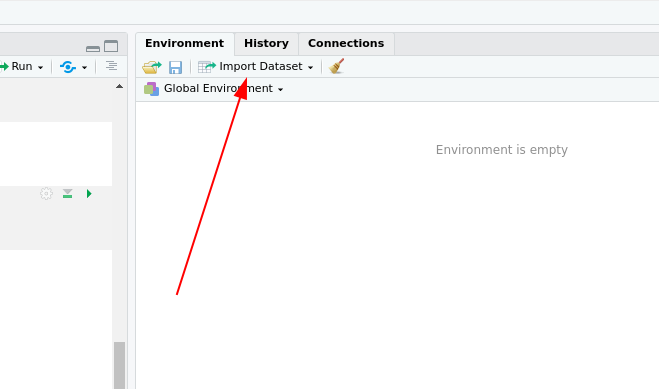
\includegraphics[width=0.8\linewidth]{imgs/menu} \end{center}

\begin{center}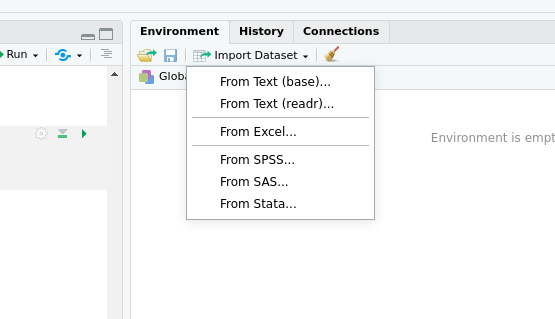
\includegraphics[width=0.8\linewidth]{imgs/menu2} \end{center}

\hypertarget{problem}{%
\subsection{Problem}\label{problem}}

Das Einlesen und Aufbereiten wird am folgenden Beispiel exerziert:
Uns interessiert der Zusammenhang von Drogenmissbrauch, Lebenszufriedenheit und Straftaten in Großbritannien. Dafür haben wir die folgenden drei Datensätz zur Verfügung:

\begin{itemize}
\item
  \texttt{\textquotesingle{}crime.csv\textquotesingle{}} - Eine Textdatei mit nach Polizeibehörde aufgeschlüsselten Straftaten
\item
  \texttt{\textquotesingle{}drugs.xlsx\textquotesingle{}} - Eine Excel-Arbeitsmappe mit nach Region aufgeschlüsselten Zahlen zu Krankenhauseinweisungen mit drogenbedingten Diagnosen
\item
  \texttt{\textquotesingle{}satisfaction.sav\textquotesingle{}} - Ein in SPSS erstellter Datensatz mit nach Region aufgeschlüsselten Ergebnissen einer Bevölkerungsbefragung zur Lebenszufriedenheit
\end{itemize}

\hypertarget{textbasierte-daten}{%
\subsection{textbasierte Daten}\label{textbasierte-daten}}

Die GUI ist hier ein guter Start. Wir wollen die Datei \texttt{\textquotesingle{}crime.csv\textquotesingle{}} einlesen. Diese enthält echte Daten über von britischen Polizeibehörden aufgezeichnete Straftaten von der \href{https://www.gov.uk/government/statistics/historical-crime-data}{Website der britischen Regierung}. Wenn ich dem Pfad im GUI folge, ergibt sich das folgende Bild:

\begin{center}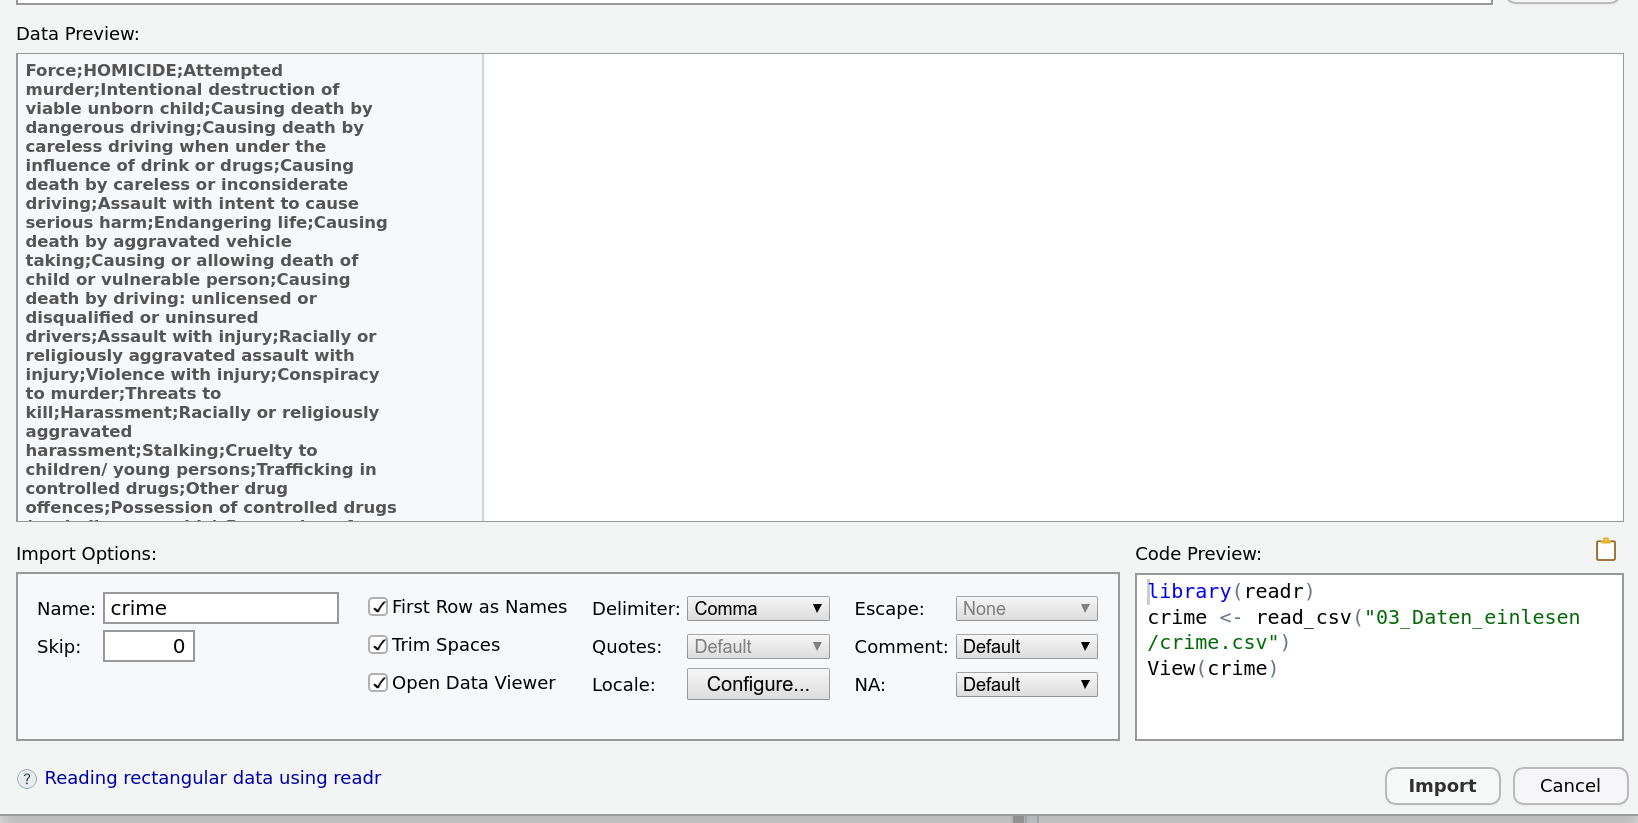
\includegraphics[width=0.8\linewidth]{imgs/text} \end{center}

Was ist das Problem?

Das Trennzeichen(Delimiter) ist falsch gesetzt. In den Daten sind die Zellen offensichtlich durch Semikolons getrennt.

\begin{center}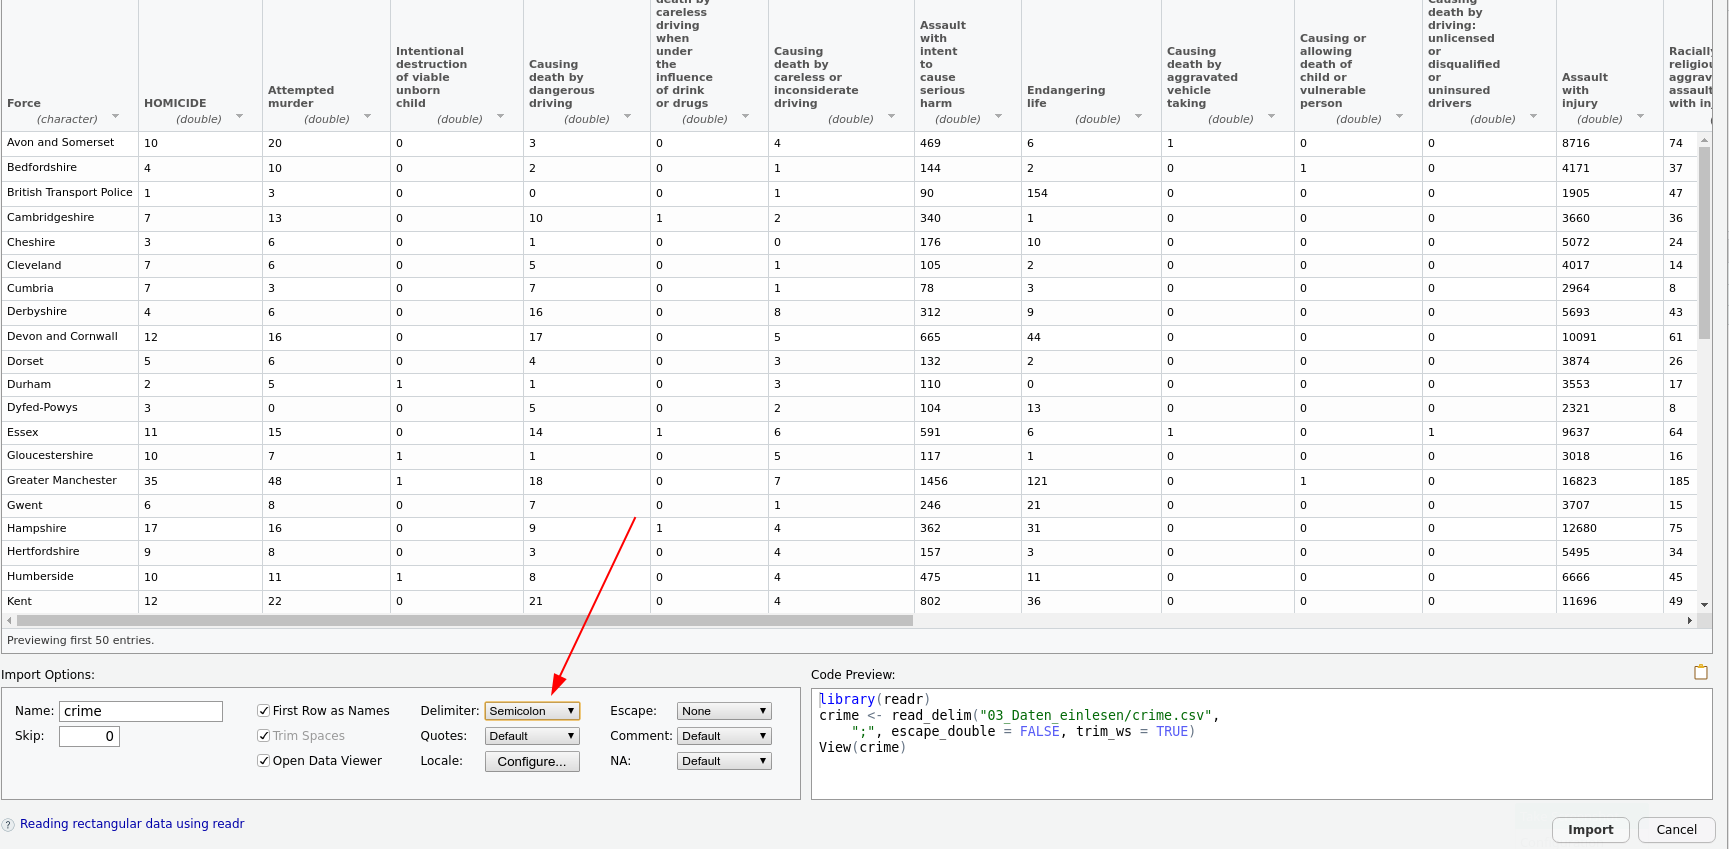
\includegraphics[width=0.8\linewidth]{imgs/text2} \end{center}

Der für das Einlesen nötige Code wird dann von RStudio in die Konsole kopiert und ausgeführt.
Um nicht jedes Mal beim Ausführen desselben Skriptes wieder per Hand den Datensatz einlesen zu müssen, kopiert man den Code dann an den Anfang des Skriptes.

\begin{center}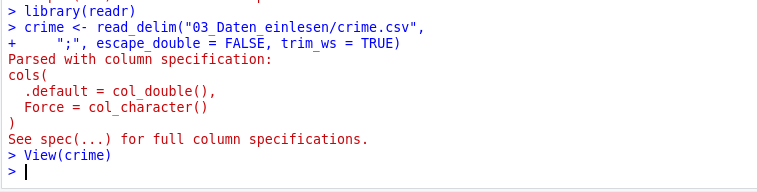
\includegraphics[width=0.8\linewidth]{imgs/text3} \end{center}

Was passiert hier?

\begin{Shaded}
\begin{Highlighting}[]
\NormalTok{crime }\OtherTok{\textless{}{-}} \FunctionTok{read\_delim}\NormalTok{(}\StringTok{"data/crime.csv"}\NormalTok{, }
\end{Highlighting}
\end{Shaded}

Lege in \texttt{crime} das Textfile mit Trennzeichen unter dem angegebenen Pfad ab. Dabei\ldots{}

\begin{Shaded}
\begin{Highlighting}[]
\StringTok{";"}\NormalTok{, escape\_double }\OtherTok{=} \ConstantTok{FALSE}\NormalTok{, trim\_ws }\OtherTok{=} \ConstantTok{TRUE}\ErrorTok{)}
\end{Highlighting}
\end{Shaded}

\ldots erwarte Semikolons als Trennzeichen, erwarte keine doppelten Anführungszeichen und schneide Leerzeichen von den Einträgen ab.

\begin{verbatim}
## 
## -- Column specification --------------------------
## cols(
##   .default = col_double(),
##   Force = col_character()
## )
## i Use `spec()` for the full column specifications.
\end{verbatim}

R teilt mit, dass es Kommazahlen als Standard-Zelleninhalt versucht und bei nicht-Funktionieren auf \texttt{character} zurückfällt. Das ist trotz der Farbe \textbf{keine} Fehlermeldung

\begin{Shaded}
\begin{Highlighting}[]
\FunctionTok{View}\NormalTok{(crime)}
\end{Highlighting}
\end{Shaded}

Dann öffne den Datensatz zum Angucken.

Noch zwei wichtige Tricks in dem Einlesetool sind die locale-Schaltfläche und das NA-Menü

\begin{center}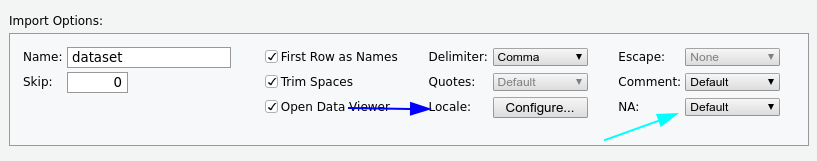
\includegraphics[width=0.8\linewidth]{imgs/text4} \end{center}

Was kann man hier anpassen?

Genau kontrollieren, ob Umlaute, Zellentrennung, fehlende Werte, Dezimaltrennzeichen,\ldots{} richtig eingestellt waren!

\hypertarget{excel-arbeitsmappen}{%
\subsection{Excel-Arbeitsmappen}\label{excel-arbeitsmappen}}

Für die Excel-Arbeitsmappen ist die GUI auch der einfachste Weg.

Wie würde man vorgehen um die Datei drugs.xlsx einzulesen?

\begin{itemize}
\tightlist
\item
  Import Dataset \(\rightarrow\) From Excel
\item
  Pfad zum file raussuchen
\end{itemize}

\begin{center}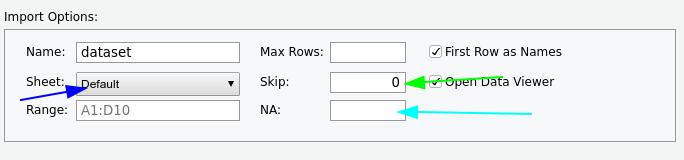
\includegraphics[width=0.8\linewidth]{imgs/excel1} \end{center}

\begin{itemize}
\tightlist
\item
  Richtiges Sheet aussuchen
\item
  unnötige Zeilen überspringen
\item
  etwaige von leeren Zellen abweichende NA-Codierung anpassen
\end{itemize}

Auch bei Excel-Mappen an das Kopieren des Codes denken!

\begin{Shaded}
\begin{Highlighting}[]
\FunctionTok{library}\NormalTok{(readxl)}
\NormalTok{drugs }\OtherTok{\textless{}{-}} \FunctionTok{read\_excel}\NormalTok{(}\StringTok{"data/drugs.xlsx"}\NormalTok{,}
                    \AttributeTok{sheet =} \StringTok{"Table 2"}\NormalTok{, }\AttributeTok{na =} \StringTok{"*"}\NormalTok{, }\AttributeTok{skip =} \DecValTok{10}\NormalTok{)}
\end{Highlighting}
\end{Shaded}

\begin{verbatim}
## New names:
## * `` -> ...1
## * `` -> ...2
## * `` -> ...3
## * `` -> ...4
\end{verbatim}

Diese Daten sind übrigens auch Originaldaten von der Website des \href{https://digital.nhs.uk/data-and-information/publications/statistical/statistics-on-drug-misuse/2018}{britischen National Health Services}

\hypertarget{dateien-aus-anderer-software}{%
\subsection{Dateien aus anderer Software}\label{dateien-aus-anderer-software}}

Beispielhaft für SPSS, für Stata etc analog.
Die GUI ist wieder ein guter Anfang und hier ziemlich selbsterklärend.

Wie würde man vorgehen um die Datei satisfaction.sav einzulesen?

\begin{Shaded}
\begin{Highlighting}[]
\FunctionTok{library}\NormalTok{(haven)}
\NormalTok{satisfaction }\OtherTok{\textless{}{-}} \FunctionTok{read\_sav}\NormalTok{(}\StringTok{"data/satisfaction.sav"}\NormalTok{)}
\end{Highlighting}
\end{Shaded}

Die Daten kommen diesmal vom britischen \href{https://www.ons.gov.uk/peoplepopulationandcommunity/wellbeing/adhocs/007955estimatesofpersonalwellbeingbrokendownbycountryofbirthfromtheukannualpopulationsurveyaps}{Office for National Statistics}, wurden aber stark abgewandelt.

\hypertarget{dateien-aus-spss-einlesen}{%
\subsection{Dateien aus SPSS einlesen}\label{dateien-aus-spss-einlesen}}

Wenn man sich die Daten in der RStudio-Oberfläche anguckt, sieht man, dass die für SPSS typischen Variablendefinitionen konserviert wurden:

\begin{center}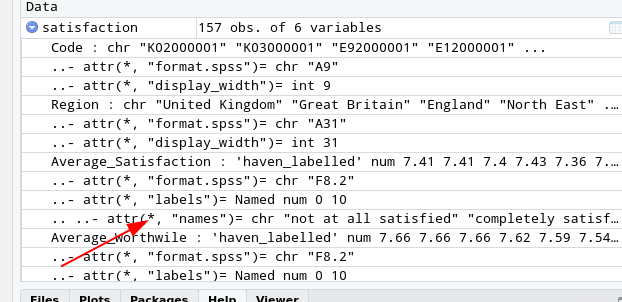
\includegraphics[width=0.8\linewidth]{imgs/spss1} \end{center}

\texttt{haven} bietet mit der \texttt{as\_factor}-Funktion eine Möglichkeit an, eine dieser Codierung enthaltenden Variablen in einen Faktor umzuwandeln.

Faktoren sind eine Variante um in R kategoriale Variablen anzulegen.

So könnten wir uns zum Beispiel entscheiden, einen neuen, zweiten Datensatz zu erstellen, der die Variablen mit den Verballabels aus SPSS enthält.
Da wir auf alle Spalten dafür dieselbe Funktion anwenden wollen, können wir dafür die \texttt{mutate\_all}-Funktion verwenden.

Dabei benutzen wir die im \texttt{tidyverse} beim Batchen von Funktionen verbreitete Funktionsschreibweise:

\begin{Shaded}
\begin{Highlighting}[]
\NormalTok{verbal\_satisfaction }\OtherTok{\textless{}{-}}\NormalTok{ satisfaction }\SpecialCharTok{\%\textgreater{}\%} 
  \FunctionTok{mutate\_all}\NormalTok{(}\SpecialCharTok{\textasciitilde{}}\FunctionTok{as\_factor}\NormalTok{(.)) }\DocumentationTok{\#\# Nach der Tilde Funktion für alle Spalten}
\DocumentationTok{\#\# Mit dem Punkt wird angegeben, wo die Variablen eingesetzt werden sollen}
\end{Highlighting}
\end{Shaded}

Das Ergebnis sieht in der Oberfläche dann so aus:

\begin{center}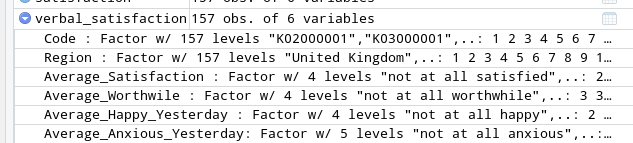
\includegraphics[width=0.8\linewidth]{imgs/spss2} \end{center}

Für Tipps zur weitergehenden Bearbeitung von SPSS und Stata-Daten noch \href{https://www.rdocumentation.org/packages/haven/versions/2.2.0/vignettes/semantics.Rmd}{hier} die sehr gute \texttt{haven}-Vignette zu den nötigen Schritten.

\hypertarget{datenaufbereitung}{%
\section{Datenaufbereitung}\label{datenaufbereitung}}

Datenaufbrereitung kann natürlich denkbar komplex sein, deswegen beschränken wir uns hier auf die folgenden Schritte:

\begin{enumerate}
\def\labelenumi{\arabic{enumi}.}
\item
  Ausreißer-Behandlung
\item
  Umgang mit fehlenden Werten
\item
  Recodieren von Werten
\end{enumerate}

\hypertarget{ausreiuxdfer-behandlung}{%
\subsection{Ausreißer-Behandlung}\label{ausreiuxdfer-behandlung}}

Als ersten Schritt zur Bereinigung der drei Datensätze sollen Ausreißer erkannt und durch fehlende Werte ausgeschlossen werden.

Dafür muss man sich natürlich zuerst überlegen, was das Kriterium dafür sein soll. Wir benutzen hier das Kriterium nach \citet{tukeyExploratoryDataAnalysis1977}, also wollen wir gerade die Werte ausschlißen, die mehr als 1.5 Interquartilabstände über oder unter dem 25\% bzw dem 75\%-Quantil liegen.

Um uns Tipparbeit zu sparen, schreiben wir dafür unsere erste Funktion:

\begin{Shaded}
\begin{Highlighting}[]
\NormalTok{remove\_outlier }\OtherTok{\textless{}{-}} \ControlFlowTok{function}\NormalTok{(x)\{}
  \FunctionTok{ifelse}\NormalTok{(}\FunctionTok{between}\NormalTok{(x,}
                 \FunctionTok{quantile}\NormalTok{(x,.}\DecValTok{25}\NormalTok{) }\SpecialCharTok{{-}} \FloatTok{1.5} \SpecialCharTok{*} \FunctionTok{IQR}\NormalTok{(x),}
                 \FunctionTok{quantile}\NormalTok{(x,.}\DecValTok{75}\NormalTok{) }\SpecialCharTok{+} \FloatTok{1.5} \SpecialCharTok{*} \FunctionTok{IQR}\NormalTok{(x)),}
\NormalTok{          x,}
          \ConstantTok{NA}\NormalTok{)\}}
\end{Highlighting}
\end{Shaded}

Kombiniert mit einem \texttt{mutate\_if} können wir damit alle Ausreißer gegen fehlende Werte austauschen. \texttt{mutate\_if} ist mit \texttt{mutate\_all} vergleichbar, nur dass man einen logischen Wert übergeben kann um die umzuwandelnden Spalten auszuwählen.

\begin{Shaded}
\begin{Highlighting}[]
\NormalTok{crime }\OtherTok{\textless{}{-}}\NormalTok{ crime }\SpecialCharTok{\%\textgreater{}\%} 
  \FunctionTok{mutate\_if}\NormalTok{(}\AttributeTok{.predicate =}\NormalTok{ is.numeric,}
            \SpecialCharTok{\textasciitilde{}}\FunctionTok{remove\_outlier}\NormalTok{(.))}
\end{Highlighting}
\end{Shaded}

\hypertarget{umgang-mit-fehlenden-werten}{%
\subsection{Umgang mit fehlenden Werten}\label{umgang-mit-fehlenden-werten}}

Fehlende Werte werden in R generell mit \texttt{NA} codiert. Um damit umzugehen bietet das \texttt{tidyverse} ein paar Funktionen, wir beschränken uns hier auf zwei.

\texttt{drop\_na} zum rigorosen Entfernen von Zeilen mit fehlenden Werten:

\begin{Shaded}
\begin{Highlighting}[]
\NormalTok{drugs }\SpecialCharTok{\%\textgreater{}\%} 
  \FunctionTok{drop\_na}\NormalTok{()}
\end{Highlighting}
\end{Shaded}

\begin{verbatim}
## # A tibble: 0 x 7
## # ... with 7 variables: ...1 <chr>, ...2 <chr>,
## #   ...3 <chr>, ...4 <chr>, `All persons9` <dbl>,
## #   Male <dbl>, Female <dbl>
\end{verbatim}

\ldots in unserem Fall vielleicht ein bisschen zu rigoros

Die zweite Möglichkeit ist \texttt{replace\_na}, eine Funktion die, wie der Name schon sagt, \texttt{NA}s durch festgelegte Werte ersetzen kann. Mit einem \texttt{mutate\_if} kombiniert, können wir so alle fehlenden Zahlen im Datensatz durch 0 ersetzen:

\begin{Shaded}
\begin{Highlighting}[]
\NormalTok{drugs }\SpecialCharTok{\%\textgreater{}\%} 
  \FunctionTok{mutate\_if}\NormalTok{(is.numeric,}\SpecialCharTok{\textasciitilde{}}\FunctionTok{replace\_na}\NormalTok{(.,}\DecValTok{0}\NormalTok{))}
\end{Highlighting}
\end{Shaded}

\begin{verbatim}
## # A tibble: 195 x 7
##   ...1  ...2  ...3  ...4  `All persons9`  Male
##   <chr> <chr> <chr> <chr>          <dbl> <dbl>
## 1 <NA>  <NA>  <NA>  <NA>               0     0
## 2 E920~ <NA>  <NA>  Engl~           7139  5294
## 3 <NA>  <NA>  <NA>  <NA>               0     0
## 4 U     <NA>  U     Unkn~            244   202
## 5 <NA>  <NA>  <NA>  <NA>               0     0
## # ... with 190 more rows, and 1 more variable:
## #   Female <dbl>
\end{verbatim}

Jetzt können wir noch die fehlenden \texttt{character} umgewandeln:

\begin{Shaded}
\begin{Highlighting}[]
\NormalTok{drugs }\OtherTok{\textless{}{-}}\NormalTok{ drugs }\SpecialCharTok{\%\textgreater{}\%} 
  \FunctionTok{mutate\_if}\NormalTok{(is.numeric,}\SpecialCharTok{\textasciitilde{}}\FunctionTok{replace\_na}\NormalTok{(.,}\DecValTok{0}\NormalTok{)) }\SpecialCharTok{\%\textgreater{}\%} 
  \FunctionTok{mutate\_if}\NormalTok{(is.character,}\SpecialCharTok{\textasciitilde{}}\FunctionTok{replace\_na}\NormalTok{(.,}\StringTok{\textquotesingle{}\textquotesingle{}}\NormalTok{))}
\NormalTok{drugs}
\end{Highlighting}
\end{Shaded}

\begin{verbatim}
## # A tibble: 195 x 7
##   ...1  ...2  ...3  ...4  `All persons9`  Male
##   <chr> <chr> <chr> <chr>          <dbl> <dbl>
## 1 ""    ""    ""    ""                 0     0
## 2 "E92~ ""    ""    "Eng~           7139  5294
## 3 ""    ""    ""    ""                 0     0
## 4 "U"   ""    "U"   "Unk~            244   202
## 5 ""    ""    ""    ""                 0     0
## # ... with 190 more rows, and 1 more variable:
## #   Female <dbl>
\end{verbatim}

\hypertarget{recodieren-von-werten}{%
\subsection{Recodieren von Werten}\label{recodieren-von-werten}}

Das Recodieren von Werten funktioniert einfach über eine \texttt{mutate}-pipeline.

Für Kategoriale Daten bietet das \texttt{tidyverse} die \texttt{recode}-Funktion, hier wollen wir uns aber auf numerische Daten beschränken.

Wie könnte ich die \emph{Anxiety}-Skala im \texttt{satisfaction}-Datensatz umpolen?

\begin{Shaded}
\begin{Highlighting}[]
\NormalTok{satisfaction }\OtherTok{\textless{}{-}}\NormalTok{ satisfaction }\SpecialCharTok{\%\textgreater{}\%} 
  \FunctionTok{mutate}\NormalTok{(}\AttributeTok{Average\_Anxious\_Yesterday =} \SpecialCharTok{{-}}\DecValTok{1}\SpecialCharTok{*}\NormalTok{ (Average\_Anxious\_Yesterday}\DecValTok{{-}10}\NormalTok{))}
\end{Highlighting}
\end{Shaded}

\hypertarget{zusammenfuxfchren-von-datensuxe4tzen}{%
\section{Zusammenführen von Datensätzen}\label{zusammenfuxfchren-von-datensuxe4tzen}}

Zu guter Letzt wollen wir die drei Datensätze zu einem Datensatz zusammenfügen.\\
Dieser soll pro Region
1. die Anzahl aller drogenbezogenen Krankenhausaufenthalte
2. die Anzahl der (versuchten) Mordfälle
3. die mittlere Zufriedenheit über alle Skalen beinhalten

Wir fangen damit an, die Datensätze wie gewünscht vorzubereiten.
Aus dem \texttt{drugs}-Datensatz brauchen wir die Regionsbezeichnung, die ONS-Codes und natürlich die Zahl der Einweisungen:

\begin{Shaded}
\begin{Highlighting}[]
\NormalTok{drugs }\OtherTok{\textless{}{-}}\NormalTok{ drugs }\SpecialCharTok{\%\textgreater{}\%} 
  \FunctionTok{select}\NormalTok{(...}\DecValTok{1}\NormalTok{,...}\DecValTok{4}\NormalTok{, }\StringTok{\textasciigrave{}}\AttributeTok{All persons9}\StringTok{\textasciigrave{}}\NormalTok{)}
\end{Highlighting}
\end{Shaded}

Aus dem \texttt{crime}-Datensatz brauchen wir die Bezeichnung der Niederlassung, Anzahl der Morde und die Anzahl der versuchten Morde:

\begin{Shaded}
\begin{Highlighting}[]
\NormalTok{crime }\OtherTok{\textless{}{-}}\NormalTok{ crime }\SpecialCharTok{\%\textgreater{}\%} 
  \FunctionTok{select}\NormalTok{(Force,HOMICIDE,}\StringTok{\textasciigrave{}}\AttributeTok{Attempted murder}\StringTok{\textasciigrave{}}\NormalTok{)}
\end{Highlighting}
\end{Shaded}

Aus dem \texttt{satisfaction}-Datensatz brauchen wir den ONS-Code und einen mittleren Zufriedenheitswert

Wie könnte ich das angehen?

\begin{Shaded}
\begin{Highlighting}[]
\NormalTok{satisfaction }\OtherTok{\textless{}{-}}\NormalTok{ satisfaction }\SpecialCharTok{\%\textgreater{}\%} 
  \FunctionTok{transmute}\NormalTok{(}\AttributeTok{Code =}\NormalTok{ Code,}
            \AttributeTok{Satisfaction =}\NormalTok{ (Average\_Satisfaction }\SpecialCharTok{+}\NormalTok{ Average\_Worthwile }\SpecialCharTok{+} 
\NormalTok{              Average\_Happy\_Yesterday }\SpecialCharTok{+}\NormalTok{Average\_Anxious\_Yesterday)}\SpecialCharTok{/}\DecValTok{4}\NormalTok{)}
\end{Highlighting}
\end{Shaded}

\texttt{sum} ist keine vektorisierte Funktion! Um eine neue Summenwert pro Zeile zu bilden, sind \texttt{+} und \texttt{/} nötig

Jetzt müssen wir das ganze nur noch zusammenfügen. Dafür benutzen wir die Familien der \texttt{join}-Funktionen

Zuerst fügen wir die Anzahl der Straftaten zu der Anzahl der Krankenhauseinweisungen hinzu. Dabei matchen wir die Regionen über das Regions-Schlüsselwort und behalten nur die Fälle, in denen in beiden Datensätzen ein Schlüsselwort auftaucht:

\begin{Shaded}
\begin{Highlighting}[]
\NormalTok{overall }\OtherTok{\textless{}{-}}\NormalTok{ drugs }\SpecialCharTok{\%\textgreater{}\%} 
  \FunctionTok{inner\_join}\NormalTok{(crime, }\AttributeTok{by =} \FunctionTok{c}\NormalTok{(}\StringTok{\textquotesingle{}...4\textquotesingle{}} \OtherTok{=} \StringTok{\textquotesingle{}Force\textquotesingle{}}\NormalTok{))}
\NormalTok{overall}
\end{Highlighting}
\end{Shaded}

\begin{verbatim}
## # A tibble: 21 x 5
##   ...1  ...4  `All persons9` HOMICIDE
##   <chr> <chr>          <dbl>    <dbl>
## 1 E100~ Cumb~             72        7
## 2 E100~ Lanc~            214       16
## 3 E100~ Nort~             44        9
## 4 E100~ Derb~             81        4
## 5 E100~ Leic~             56        6
## # ... with 16 more rows, and 1 more variable:
## #   `Attempted murder` <dbl>
\end{verbatim}

Dem \texttt{overall}-Datensatz fügen wir jetzt noch die \texttt{satisfaction} hinzu. Hierzu nutzen wir die ONS-Codes. Dabei wollen wir alle Fälle in \texttt{overall} behalten:

\begin{Shaded}
\begin{Highlighting}[]
\NormalTok{overall }\OtherTok{\textless{}{-}}\NormalTok{ overall }\SpecialCharTok{\%\textgreater{}\%} 
  \FunctionTok{left\_join}\NormalTok{(satisfaction, }\AttributeTok{by =} \FunctionTok{c}\NormalTok{(}\StringTok{\textquotesingle{}...1\textquotesingle{}} \OtherTok{=} \StringTok{\textquotesingle{}Code\textquotesingle{}}\NormalTok{))}
\NormalTok{overall}
\end{Highlighting}
\end{Shaded}

\begin{verbatim}
## # A tibble: 21 x 6
##   ...1  ...4  `All persons9` HOMICIDE
##   <chr> <chr>          <dbl>    <dbl>
## 1 E100~ Cumb~             72        7
## 2 E100~ Lanc~            214       16
## 3 E100~ Nort~             44        9
## 4 E100~ Derb~             81        4
## 5 E100~ Leic~             56        6
## # ... with 16 more rows, and 2 more variables:
## #   `Attempted murder` <dbl>, Satisfaction <dbl>
\end{verbatim}

Alles was jetzt noch fehlt, sind schönere Spaltennamen. Dafür benutzen wir entweder \texttt{rename}.
\texttt{rename} erwartet die Angabe jedes Namens, der geändert werden soll als Wert und die neuen Namen als Namen der Argumente:

\begin{Shaded}
\begin{Highlighting}[]
\NormalTok{overall }\OtherTok{\textless{}{-}}\NormalTok{ overall }\SpecialCharTok{\%\textgreater{}\%} 
  \FunctionTok{rename}\NormalTok{(}\StringTok{\textquotesingle{}ONS\_Code\textquotesingle{}} \OtherTok{=} \StringTok{\textquotesingle{}...1\textquotesingle{}}\NormalTok{,}
         \StringTok{\textquotesingle{}region\textquotesingle{}} \OtherTok{=} \StringTok{\textquotesingle{}...4\textquotesingle{}}\NormalTok{,}
         \StringTok{\textquotesingle{}admissions\textquotesingle{}} \OtherTok{=} \StringTok{\textquotesingle{}All persons9\textquotesingle{}}\NormalTok{,}
         \StringTok{\textquotesingle{}homicide\textquotesingle{}} \OtherTok{=} \StringTok{\textquotesingle{}HOMICIDE\textquotesingle{}}\NormalTok{)}
\end{Highlighting}
\end{Shaded}

Damit ist unser Datensatz fertig:

\begin{Shaded}
\begin{Highlighting}[]
\NormalTok{overall}
\end{Highlighting}
\end{Shaded}

\begin{verbatim}
## # A tibble: 21 x 6
##   ONS_Code region admissions homicide
##   <chr>    <chr>       <dbl>    <dbl>
## 1 E100000~ Cumbr~         72        7
## 2 E100000~ Lanca~        214       16
## 3 E100000~ North~         44        9
## 4 E100000~ Derby~         81        4
## 5 E100000~ Leice~         56        6
## # ... with 16 more rows, and 2 more variables:
## #   `Attempted murder` <dbl>, Satisfaction <dbl>
\end{verbatim}

Den speichern wir noch eben als csv-Datei ab.

\begin{Shaded}
\begin{Highlighting}[]
\NormalTok{overall }\SpecialCharTok{\%\textgreater{}\%} \FunctionTok{write\_csv}\NormalTok{(}\StringTok{\textquotesingle{}data/drugs\_crime\_UK.csv\textquotesingle{}}\NormalTok{)}
\end{Highlighting}
\end{Shaded}

\hypertarget{daten-darstellen}{%
\chapter{Daten darstellen}\label{daten-darstellen}}

\hypertarget{pivotieren-von-datensuxe4tzen}{%
\section{pivotieren von Datensätzen}\label{pivotieren-von-datensuxe4tzen}}

Als Vorbereitung auf die Darstellung von Daten brauchen wir noch eine Funktion.

Für das Grafikpaket, das wir benutzen wollen, müssen die Daten im \texttt{long\ format} vorliegen. Das heißt, dass jede Variable eine Spalte und jede Zeile eine Beobachtung darstellt.

Insbesondere müssen wir darauf achten, dass alle Werte, die wir zum Beispiel an einer Achse darstellen wollen in einer Variable vorliegen.

Als Beispiel wollen wir den \texttt{\textquotesingle{}crime\textquotesingle{}}-Datensatz pivotieren. Um das ganze übersichtlicher zu halten, bereiten wir den Datensatz aber noch ein bisschen vor.

Wir wollen dafür

\begin{enumerate}
\def\labelenumi{\arabic{enumi}.}
\tightlist
\item
  Den Datensatz einlesen
\item
  Die Spalten \texttt{Force}, \texttt{HOMICIDE}, \texttt{Attempted\ murder}, \texttt{Violence\ with\ injury} und \texttt{Assault\ with\ injury} einlesen.
\item
  Die Mord-Spalte so umbenennen, dass der Name in das restliche Schema passt.
\item
  Die \texttt{Total}-Zeile ausschließen.
\end{enumerate}

Wie machen wir das?

\begin{Shaded}
\begin{Highlighting}[]
\FunctionTok{library}\NormalTok{(tidyverse)}
\NormalTok{crime }\OtherTok{\textless{}{-}} \FunctionTok{read\_delim}\NormalTok{(}\StringTok{"data/crime\_plot.csv"}\NormalTok{, }
                    \StringTok{";"}\NormalTok{, }\AttributeTok{escape\_double =} \ConstantTok{FALSE}\NormalTok{, }\AttributeTok{trim\_ws =} \ConstantTok{TRUE}\NormalTok{) }\SpecialCharTok{\%\textgreater{}\%} 
  \FunctionTok{select}\NormalTok{(Force,HOMICIDE,Country,}\StringTok{\textasciigrave{}}\AttributeTok{Attempted murder}\StringTok{\textasciigrave{}}\NormalTok{, }
         \StringTok{\textasciigrave{}}\AttributeTok{Violence with injury}\StringTok{\textasciigrave{}}\NormalTok{, }\StringTok{\textasciigrave{}}\AttributeTok{Assault with injury}\StringTok{\textasciigrave{}}\NormalTok{) }\SpecialCharTok{\%\textgreater{}\%} 
  \FunctionTok{rename}\NormalTok{(}\StringTok{\textquotesingle{}Homicide\textquotesingle{}} \OtherTok{=} \StringTok{\textquotesingle{}HOMICIDE\textquotesingle{}}\NormalTok{) }\SpecialCharTok{\%\textgreater{}\%} 
  \FunctionTok{filter}\NormalTok{(Force }\SpecialCharTok{!=} \StringTok{\textquotesingle{}Total\textquotesingle{}}\NormalTok{)}
\FunctionTok{glimpse}\NormalTok{(crime)}
\end{Highlighting}
\end{Shaded}

\begin{verbatim}
## Rows: 44
## Columns: 6
## $ Force                  <chr> "Avon and Some...
## $ Homicide               <dbl> 10, 4, 1, 7, 3...
## $ Country                <chr> "England", "En...
## $ `Attempted murder`     <dbl> 20, 10, 3, 13,...
## $ `Violence with injury` <dbl> 9293, 4368, 22...
## $ `Assault with injury`  <dbl> 8716, 4171, 19...
\end{verbatim}

Um den Datensatz in ein längeres Format zu pivotieren, benutzen wir die \texttt{pivot\_longer}-Funktion.
Wir erstellen dafür hier einen zweiten Datensatz

\begin{Shaded}
\begin{Highlighting}[]
\NormalTok{crime\_long }\OtherTok{\textless{}{-}}\NormalTok{ crime }\SpecialCharTok{\%\textgreater{}\%} 
  \FunctionTok{pivot\_longer}\NormalTok{(}
    \AttributeTok{cols =} \FunctionTok{c}\NormalTok{(}\StringTok{\textquotesingle{}Homicide\textquotesingle{}}\NormalTok{,}\StringTok{\textquotesingle{}Attempted murder\textquotesingle{}}\NormalTok{, }
             \StringTok{\textquotesingle{}Violence with injury\textquotesingle{}}\NormalTok{, }\StringTok{\textquotesingle{}Assault with injury\textquotesingle{}}\NormalTok{),}
    \AttributeTok{names\_to =} \StringTok{\textquotesingle{}offence\textquotesingle{}}\NormalTok{, }
    \AttributeTok{values\_to =} \StringTok{\textquotesingle{}count\textquotesingle{}}\NormalTok{)}
\FunctionTok{glimpse}\NormalTok{(crime\_long)}
\end{Highlighting}
\end{Shaded}

\begin{verbatim}
## Rows: 176
## Columns: 4
## $ Force   <chr> "Avon and Somerset", "Avon an...
## $ Country <chr> "England", "England", "Englan...
## $ offence <chr> "Homicide", "Attempted murder...
## $ count   <dbl> 10, 20, 9293, 8716, 4, 10, 43...
\end{verbatim}

\hypertarget{vorbereitung-fuxfcr-die-grafische-darstellung}{%
\subsection{Vorbereitung für die grafische Darstellung}\label{vorbereitung-fuxfcr-die-grafische-darstellung}}

Abschließend fügen wir noch für später Auswertungen eine Variable hinzu, die codiert, ob die Straftat in einer Verletzung ausgegangen ist oder versuchter/erfolgreicher Mord ist. Dafür benutzen wir die \texttt{str\_detect}-Funktion.

\begin{Shaded}
\begin{Highlighting}[]
\NormalTok{crime\_long }\OtherTok{\textless{}{-}}\NormalTok{ crime\_long }\SpecialCharTok{\%\textgreater{}\%} 
  \FunctionTok{mutate}\NormalTok{(}\AttributeTok{type\_of\_offence =} \FunctionTok{ifelse}\NormalTok{(}\FunctionTok{str\_detect}\NormalTok{(offence, }\StringTok{\textquotesingle{}injury\textquotesingle{}}\NormalTok{),}
                                  \StringTok{\textquotesingle{}injury\textquotesingle{}}\NormalTok{,}
                                  \StringTok{\textquotesingle{}(attempted) homicide\textquotesingle{}}\NormalTok{))}
\FunctionTok{glimpse}\NormalTok{(crime)}
\end{Highlighting}
\end{Shaded}

\begin{verbatim}
## Rows: 44
## Columns: 6
## $ Force                  <chr> "Avon and Some...
## $ Homicide               <dbl> 10, 4, 1, 7, 3...
## $ Country                <chr> "England", "En...
## $ `Attempted murder`     <dbl> 20, 10, 3, 13,...
## $ `Violence with injury` <dbl> 9293, 4368, 22...
## $ `Assault with injury`  <dbl> 8716, 4171, 19...
\end{verbatim}

\hypertarget{ggplot2}{%
\section{ggplot2}\label{ggplot2}}

Eins der stärksten Argumente für die Benutzung von R und dem \texttt{tidyverse} ist das Grafik-Paket \texttt{ggplot2}.

Mit ein bisschen Gewöhnung macht \texttt{ggplot2} es sehr einfach, hübsche Grafiken zu erstellen.

Die Syntax für \texttt{ggplot2} ist dabei aber ein bisschen anders als die, die wir bisher von R gewohnt sind.

Dafür müssen wir zuerst eine Grundebene erstellen, auf die wir die Grafik anschließend layern können.

Diese Grundebene kann man sich ein bisschen wie eine leere Leinwand vorstellen.
Dabei wird beim Erstellen der `Leinwand' direkt festgelegt, auf welchen Daten die Abbildung basieren soll und welche Variablen wie dargestellt werden sollen.

Diese Leinwand erstellt man mit der \texttt{ggplot}-Funktion, in die man, wie in die meisten \texttt{tidyverse}-Funktionen, pipen kann.

Als zweites Argument nach dem Datensatz erwartet \texttt{ggplot} eine Angabe, wie welche Variablen dargestellt werden sollen. Diese Angaben \emph{müssen} mit \texttt{aes} für aesthetics erstellt werden:

\begin{Shaded}
\begin{Highlighting}[]
\NormalTok{crime\_plot }\OtherTok{\textless{}{-}}\NormalTok{ crime }\SpecialCharTok{\%\textgreater{}\%} 
  \FunctionTok{ggplot}\NormalTok{(}\FunctionTok{aes}\NormalTok{(}\AttributeTok{x =}\NormalTok{ Homicide, }\AttributeTok{y =} \StringTok{\textasciigrave{}}\AttributeTok{Attempted murder}\StringTok{\textasciigrave{}}\NormalTok{))}
\end{Highlighting}
\end{Shaded}

Diese `leere Leinwand' sieht so aus:

\begin{Shaded}
\begin{Highlighting}[]
\NormalTok{crime\_plot}
\end{Highlighting}
\end{Shaded}

\begin{center}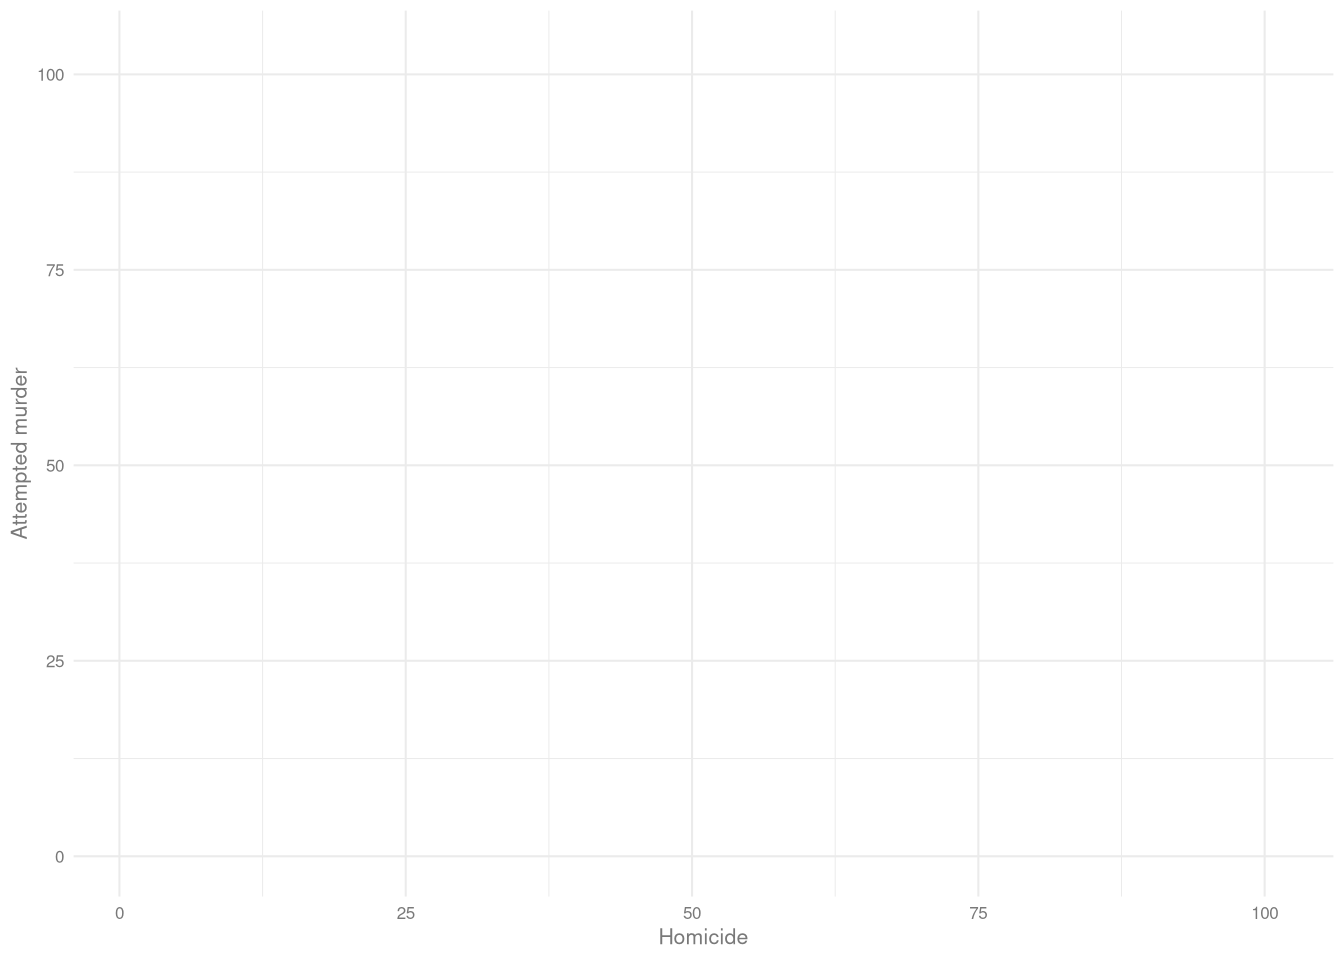
\includegraphics[width=333.333333333333pt]{R_Einfuehrung_111220_files/figure-latex/unnamed-chunk-94-1} \end{center}

\hypertarget{aesthetics}{%
\subsection{aesthetics}\label{aesthetics}}

Auf diese Leinwand können wir dann eine Reihe von verschiedenen grafischen Elementen legen, den so genannten \texttt{geom}s. Das einfachste Beispiel auf der eben erstellten Leinwand ist ein Scatterplot.
Um der Leinwand Punkte hinzuzufügen, \emph{addieren} wir einfach einen \texttt{geom\_point}-Layer auf die Grafik:

\begin{Shaded}
\begin{Highlighting}[]
\NormalTok{crime\_plot }\SpecialCharTok{+} \FunctionTok{geom\_point}\NormalTok{()}
\end{Highlighting}
\end{Shaded}

\begin{center}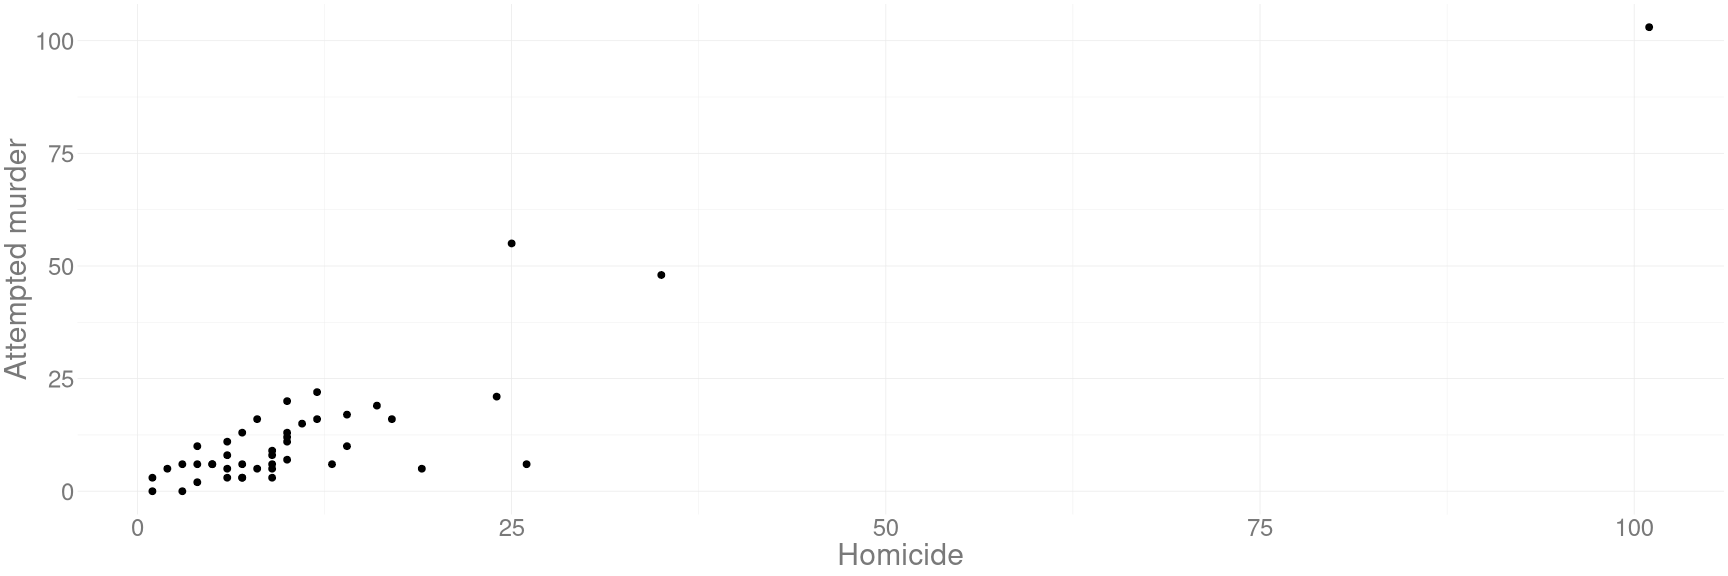
\includegraphics[width=333.333333333333pt]{imgs/pts} \end{center}

Dieser sehr einfache Graph ist aber natürlich nicht alles. Die \texttt{aes}- und die \texttt{ggplot}-Funktionen können noch eine ganze Reihe an weiteren grafischen Parametern annehmen.

Die für unseren Graphen attraktivsten sind:

\begin{itemize}
\tightlist
\item
  \texttt{size} - für die Punktgröße
\item
  \texttt{color} - für die Farbe der Punkte
\item
  \texttt{shape} - für die Wahl der Symbole
\end{itemize}

Jedes \texttt{geom} hat auch die Möglichkeit, Daten und \texttt{aesthetics} zu nehmen. Wenn keine gesetzt werden, werden einfach die des ursprünglichen \texttt{ggplot}-Aufrufs übernommen.

\begin{Shaded}
\begin{Highlighting}[]
\NormalTok{crime\_plot }\SpecialCharTok{+} \FunctionTok{geom\_point}\NormalTok{(}\FunctionTok{aes}\NormalTok{(}\AttributeTok{size =} \StringTok{\textasciigrave{}}\AttributeTok{Violence with injury}\StringTok{\textasciigrave{}}\NormalTok{, }
                            \AttributeTok{color =} \StringTok{\textasciigrave{}}\AttributeTok{Assault with injury}\StringTok{\textasciigrave{}}\NormalTok{))}
\end{Highlighting}
\end{Shaded}

\begin{center}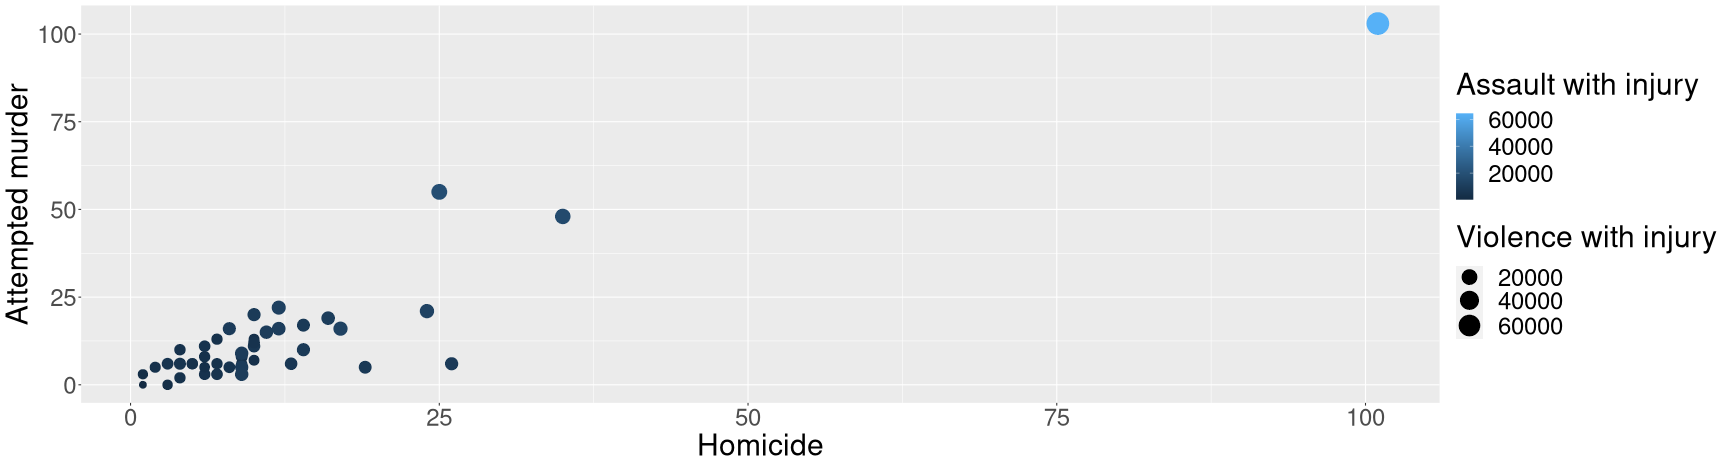
\includegraphics[width=333.333333333333pt]{imgs/pts2} \end{center}

Die aus mehreren Worten bestehenden Variablennamen sind mit Gravis eingeschlossen, nicht mit Anführungszeichen!

Wenn \texttt{aesthetic}-Argumente außerhalb der \texttt{aes}-Funktion gesetzt werden, geben sie einen konstanten Wert für das \texttt{geom} an:

\begin{Shaded}
\begin{Highlighting}[]
\NormalTok{crime\_plot }\SpecialCharTok{+} \FunctionTok{geom\_point}\NormalTok{(}\FunctionTok{aes}\NormalTok{(}\AttributeTok{size =} \StringTok{\textasciigrave{}}\AttributeTok{Violence with injury}\StringTok{\textasciigrave{}}\NormalTok{), }
                            \AttributeTok{color =} \StringTok{\textquotesingle{}purple\textquotesingle{}}\NormalTok{)}
\end{Highlighting}
\end{Shaded}

\begin{center}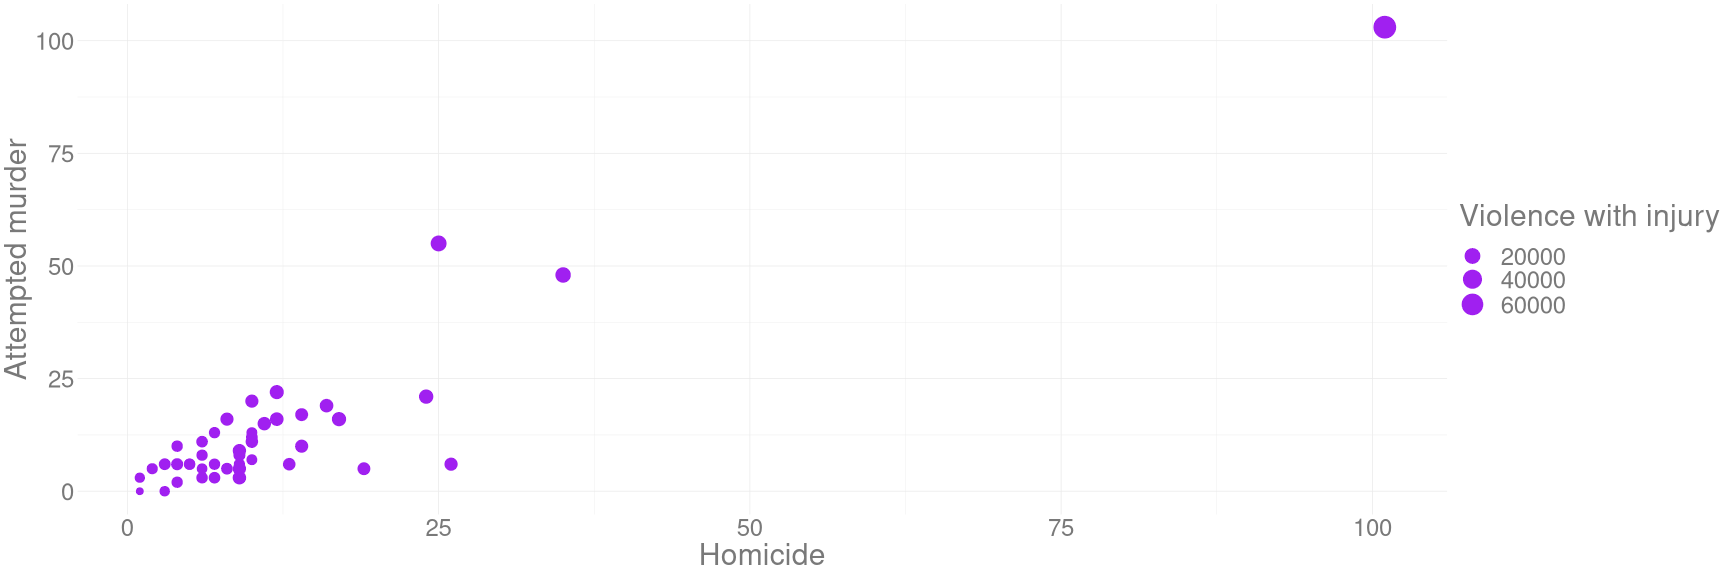
\includegraphics[width=333.333333333333pt]{imgs/pts3} \end{center}

\hypertarget{geoms}{%
\subsection{geoms}\label{geoms}}

Um andere Grafiken zu erstellen, ersetzt man einfach das \texttt{geom\_point}-geom durch ein anderes.

Dabei kann es natürlich nötig sein, eine andere Leinwand zu definieren.

Histogramme, Boxplots und Barcharts: \footnote{Für über eine Übersicht über mehr mögliche geoms lässt sich das \href{https://raw.githubusercontent.com/rstudio/cheatsheets/master/data-visualization-2.1.pdf}{ggplot2-cheatsheet} empfehlen.}

\begin{Shaded}
\begin{Highlighting}[]
\NormalTok{crime }\SpecialCharTok{\%\textgreater{}\%} 
  \FunctionTok{ggplot}\NormalTok{(}\FunctionTok{aes}\NormalTok{(}\AttributeTok{x =}\NormalTok{ Homicide)) }\SpecialCharTok{+}
  \FunctionTok{geom\_histogram}\NormalTok{(}\AttributeTok{fill =} \StringTok{\textquotesingle{}white\textquotesingle{}}\NormalTok{,}
                 \AttributeTok{color =} \StringTok{\textquotesingle{}black\textquotesingle{}}\NormalTok{,}
                 \AttributeTok{binwidth =} \DecValTok{3}\NormalTok{)}
\end{Highlighting}
\end{Shaded}

\begin{center}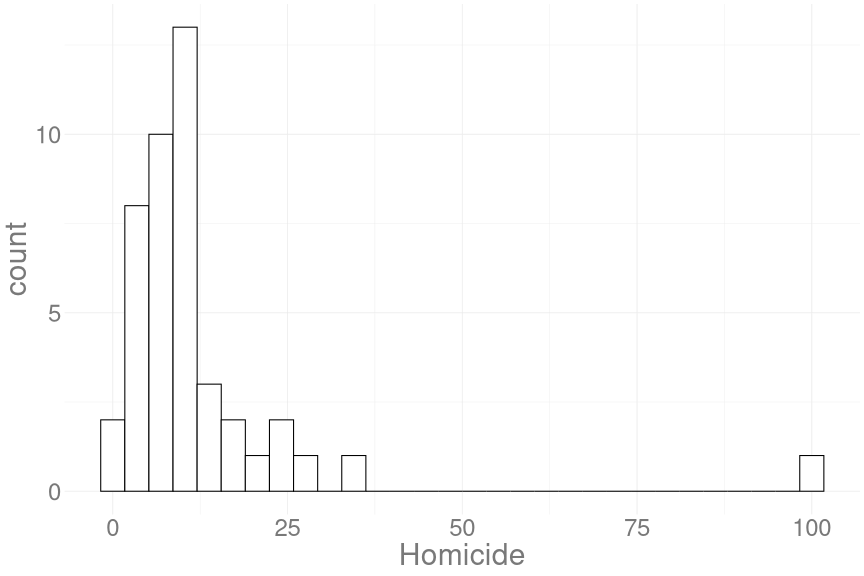
\includegraphics[width=333.333333333333pt]{imgs/pts4} \end{center}

\begin{Shaded}
\begin{Highlighting}[]
\NormalTok{crime\_long }\SpecialCharTok{\%\textgreater{}\%} 
  \FunctionTok{ggplot}\NormalTok{(}\FunctionTok{aes}\NormalTok{(}\AttributeTok{y =}\NormalTok{ count, }
             \AttributeTok{x =}\NormalTok{ offence)) }\SpecialCharTok{+}
  \FunctionTok{geom\_boxplot}\NormalTok{()}
\end{Highlighting}
\end{Shaded}

\begin{center}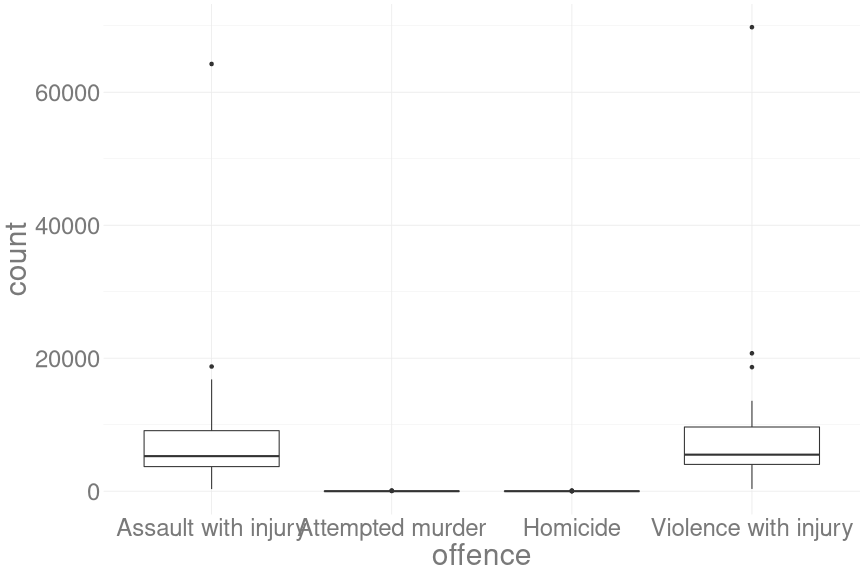
\includegraphics[width=333.333333333333pt]{imgs/pts5} \end{center}

\begin{Shaded}
\begin{Highlighting}[]
\NormalTok{crime\_long }\SpecialCharTok{\%\textgreater{}\%}
  \FunctionTok{ggplot}\NormalTok{(}\FunctionTok{aes}\NormalTok{(}\AttributeTok{y =}\NormalTok{ count,}
             \AttributeTok{x =}\NormalTok{ offence}
\NormalTok{             )) }\SpecialCharTok{+}
  \FunctionTok{geom\_col}\NormalTok{()}
\end{Highlighting}
\end{Shaded}

\begin{center}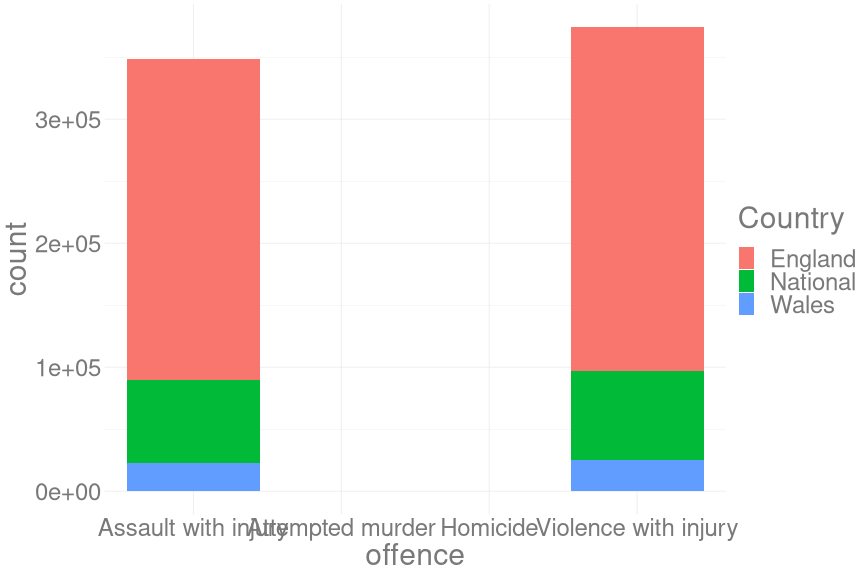
\includegraphics[width=333.333333333333pt]{imgs/pts6} \end{center}

\hypertarget{aesthetics-1}{%
\subsection{aesthetics}\label{aesthetics-1}}

Der Barchart ist ein guter Anlass, den Plot zu optimieren.

Uns stehen die folgenden Informationen zur Verfügung:

\begin{Shaded}
\begin{Highlighting}[]
\FunctionTok{glimpse}\NormalTok{(crime\_long)}
\end{Highlighting}
\end{Shaded}

\begin{verbatim}
## Rows: 176
## Columns: 5
## $ Force           <chr> "Avon and Somerset", ...
## $ Country         <chr> "England", "England",...
## $ offence         <chr> "Homicide", "Attempte...
## $ count           <dbl> 10, 20, 9293, 8716, 4...
## $ type_of_offence <chr> "(attempted) homicide...
\end{verbatim}

Um ein bisschen mehr Spielraum zu haben, gibt es in \texttt{ggplot} \texttt{facets}.

\hypertarget{facets}{%
\subsection{facets!}\label{facets}}

Facets lassen uns einfach mehrere Subplots definieren, um zusätzlich zu den in unseren \texttt{geom}s und \texttt{aes}-Aufrufen definierten Aspekten Subgruppen darzustellen.

\begin{Shaded}
\begin{Highlighting}[]
\NormalTok{crime\_long }\SpecialCharTok{\%\textgreater{}\%}  
  \FunctionTok{ggplot}\NormalTok{(}\FunctionTok{aes}\NormalTok{(}\AttributeTok{y =}\NormalTok{ count,}
             \AttributeTok{x =}\NormalTok{ Force)) }\SpecialCharTok{+}
  \FunctionTok{geom\_col}\NormalTok{(}\AttributeTok{fill =} \StringTok{\textquotesingle{}white\textquotesingle{}}\NormalTok{,}
           \AttributeTok{color =} \StringTok{\textquotesingle{}grey\textquotesingle{}}\NormalTok{) }\SpecialCharTok{+}
  \FunctionTok{facet\_grid}\NormalTok{(offence}\SpecialCharTok{\textasciitilde{}}\NormalTok{Country, }\DocumentationTok{\#\# als facets mit Straftat in Zeilen und Landesteil in Spalten}
             \AttributeTok{scales =} \StringTok{\textquotesingle{}free\textquotesingle{}}\NormalTok{) }\DocumentationTok{\#\# mit individuellen Skalen}
\end{Highlighting}
\end{Shaded}

\begin{center}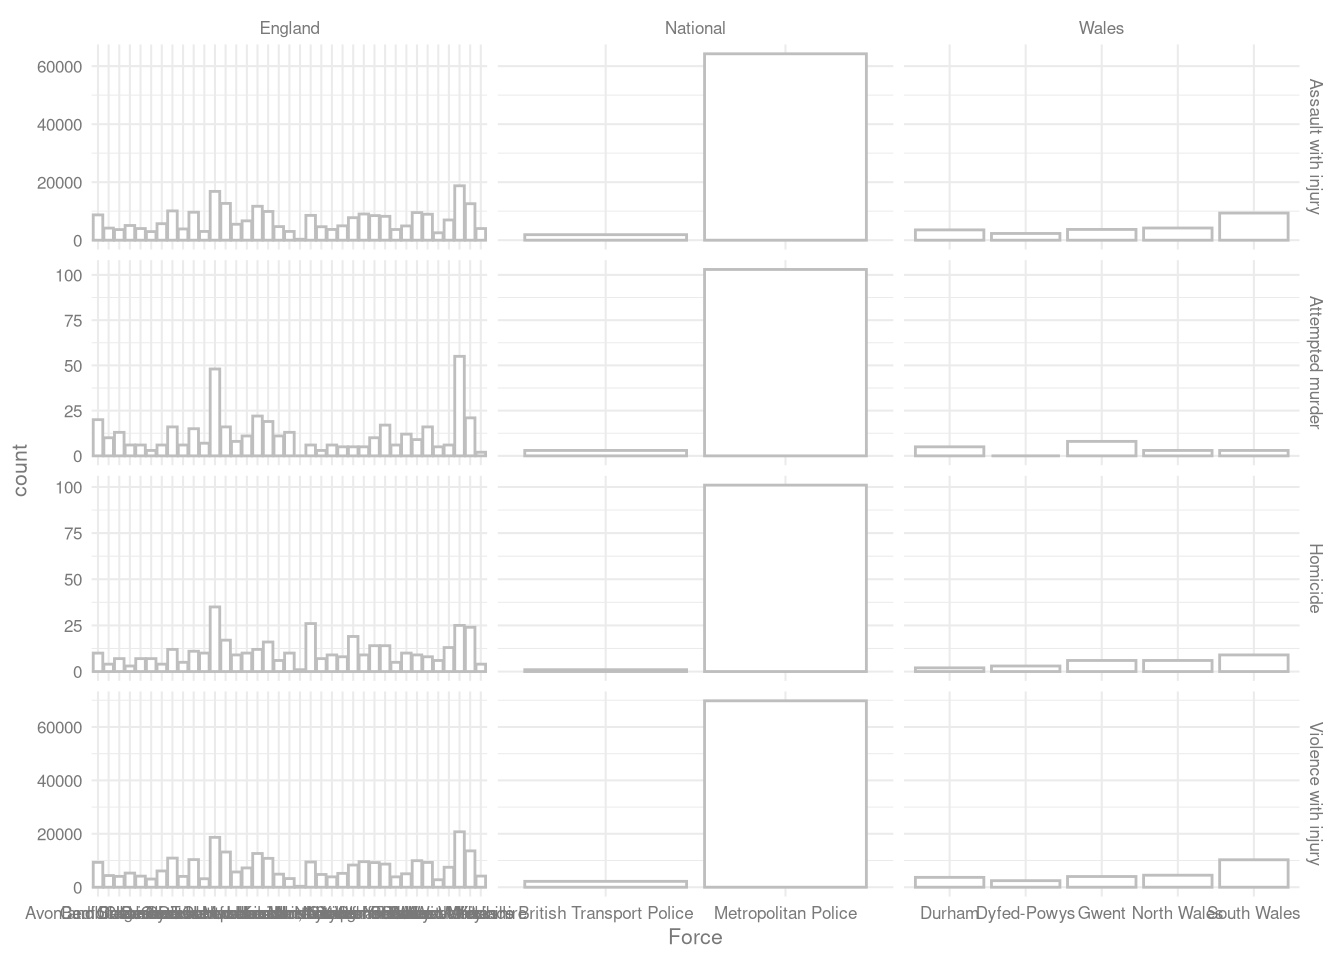
\includegraphics[width=333.333333333333pt]{R_Einfuehrung_111220_files/figure-latex/unnamed-chunk-107-1} \end{center}

Wie können wir das noch verbessern?

\hypertarget{additional-tweeks}{%
\subsection{additional tweeks}\label{additional-tweeks}}

Zuerst sortieren wir die Polizeistationen in absteigender Reihenfolge der jeweiligen mittleren Fallzahlen.

Dafür benutzen wir das \texttt{forcats}-Paket aus dem \texttt{tidyverse}. Ein Paket, dass Funktionen zum Verändern und Sortieren von Faktoren bietet.

\begin{Shaded}
\begin{Highlighting}[]
\NormalTok{crime\_long }\SpecialCharTok{\%\textgreater{}\%} 
  \FunctionTok{mutate}\NormalTok{(}
      \AttributeTok{Force =} \FunctionTok{as\_factor}\NormalTok{(Force), }\DocumentationTok{\#\# zuerst in Faktor umwandeln}
      \AttributeTok{Force =} \FunctionTok{fct\_reorder}\NormalTok{(Force, count,}\AttributeTok{.fun =}\NormalTok{ mean, }\AttributeTok{.desc =}\NormalTok{ T)) }\SpecialCharTok{\%\textgreater{}\%} \DocumentationTok{\#\# dann absteigend sortieren}
\FunctionTok{ggplot}\NormalTok{(}\FunctionTok{aes}\NormalTok{(}\AttributeTok{y =}\NormalTok{ count,}
             \AttributeTok{x =}\NormalTok{ Force)) }\SpecialCharTok{+}
  \FunctionTok{geom\_col}\NormalTok{(}\AttributeTok{fill =} \StringTok{\textquotesingle{}white\textquotesingle{}}\NormalTok{,}
           \AttributeTok{color =} \StringTok{\textquotesingle{}grey\textquotesingle{}}\NormalTok{) }\SpecialCharTok{+}
  \FunctionTok{facet\_grid}\NormalTok{(offence}\SpecialCharTok{\textasciitilde{}}\NormalTok{Country, }
             \AttributeTok{scales =} \StringTok{\textquotesingle{}free\textquotesingle{}}\NormalTok{)}
\end{Highlighting}
\end{Shaded}

\begin{center}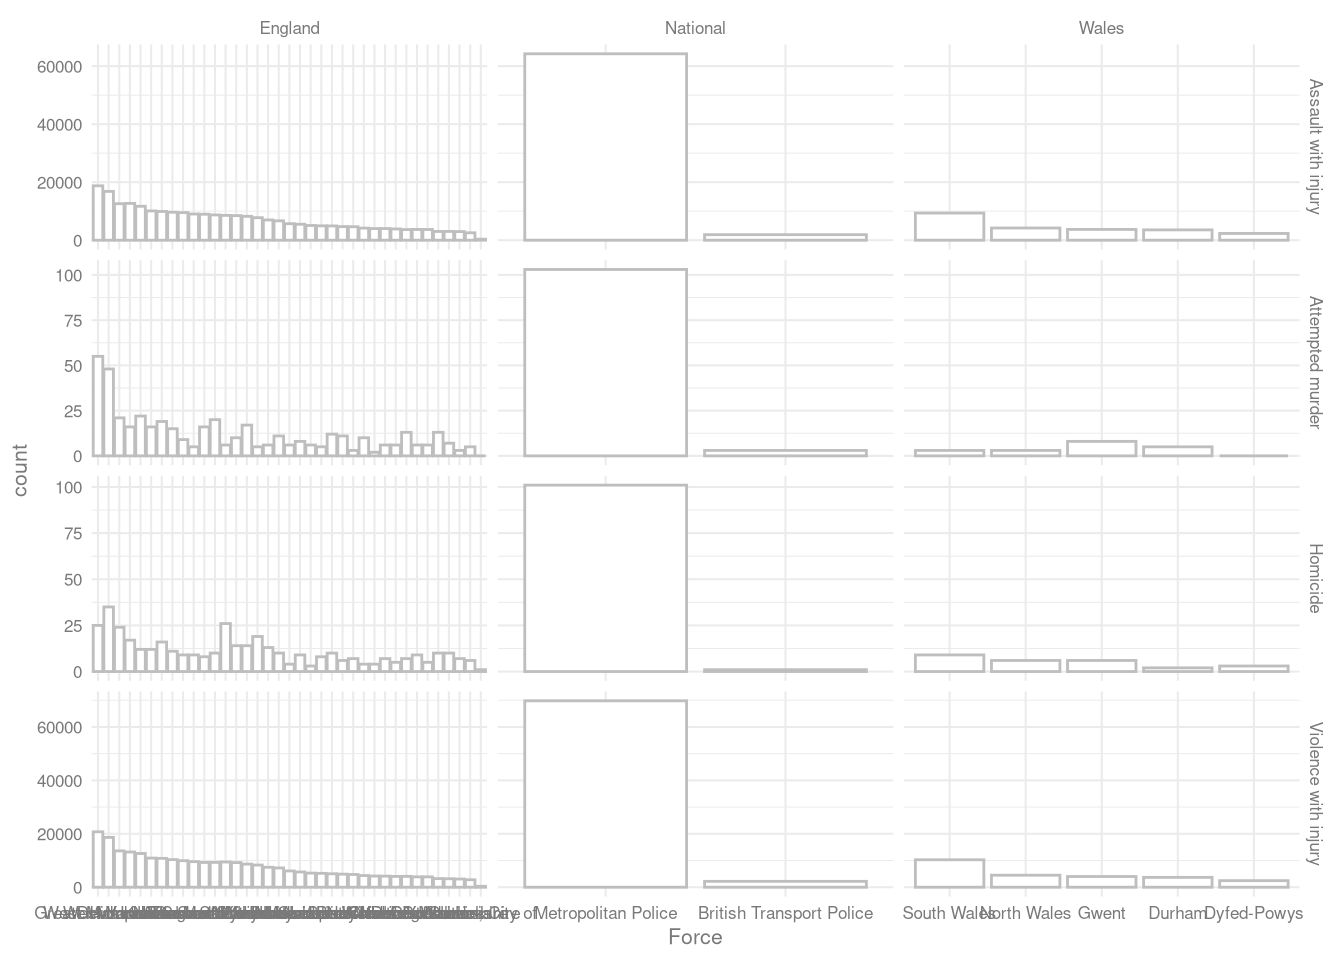
\includegraphics[width=333.333333333333pt]{R_Einfuehrung_111220_files/figure-latex/unnamed-chunk-108-1} \end{center}

Um die einzelnen Stationen besser lesbar zu machen, können wir noch die Achsen austauschen.

\begin{Shaded}
\begin{Highlighting}[]
\NormalTok{crime\_long }\SpecialCharTok{\%\textgreater{}\%} 
  \FunctionTok{mutate}\NormalTok{(}
      \AttributeTok{Force =} \FunctionTok{as\_factor}\NormalTok{(Force), }\DocumentationTok{\#\# zuerst in Faktor umwandeln}
      \AttributeTok{Force =} \FunctionTok{fct\_reorder}\NormalTok{(Force, count,}\AttributeTok{.fun =}\NormalTok{ mean, }\AttributeTok{.desc =}\NormalTok{ T)) }\SpecialCharTok{\%\textgreater{}\%} \DocumentationTok{\#\# dann absteigend sortieren}
\FunctionTok{ggplot}\NormalTok{(}\FunctionTok{aes}\NormalTok{(}\AttributeTok{y =}\NormalTok{ count,}
             \AttributeTok{x =}\NormalTok{ Force)) }\SpecialCharTok{+}
  \FunctionTok{geom\_col}\NormalTok{(}\AttributeTok{fill =} \StringTok{\textquotesingle{}white\textquotesingle{}}\NormalTok{,}
           \AttributeTok{color =} \StringTok{\textquotesingle{}grey\textquotesingle{}}\NormalTok{) }\SpecialCharTok{+}
  \FunctionTok{coord\_flip}\NormalTok{() }\SpecialCharTok{+}
  \FunctionTok{facet\_grid}\NormalTok{(Country }\SpecialCharTok{\textasciitilde{}}\NormalTok{ offence, }
             \AttributeTok{scales =} \StringTok{\textquotesingle{}free\textquotesingle{}}\NormalTok{)}
\end{Highlighting}
\end{Shaded}

\begin{center}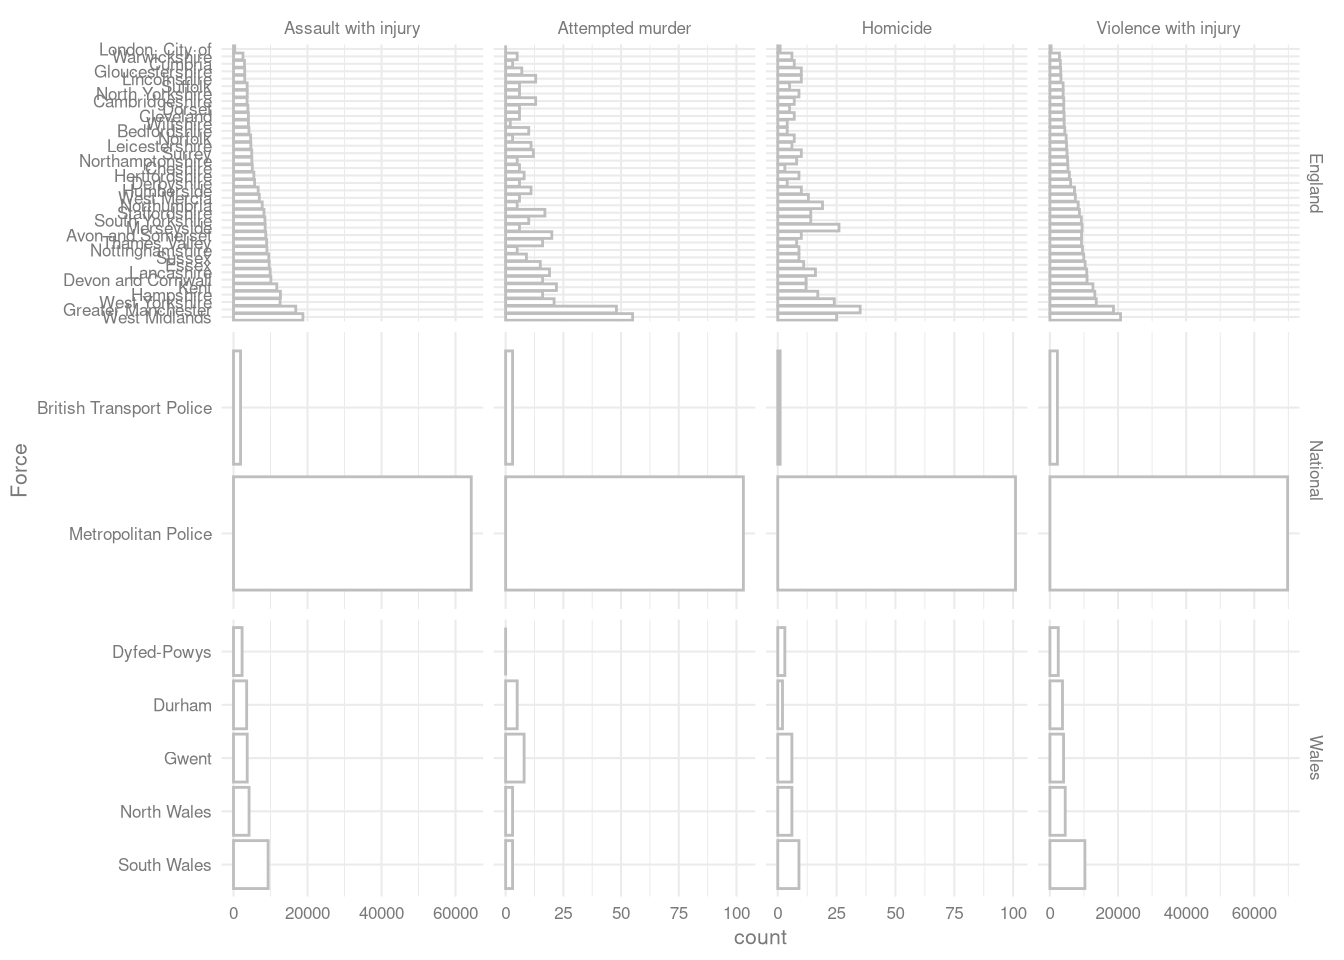
\includegraphics[width=333.333333333333pt]{R_Einfuehrung_111220_files/figure-latex/unnamed-chunk-109-1} \end{center}

\hypertarget{themes}{%
\subsection{themes}\label{themes}}

Und zuletzt die Achsenbeschriftungen anpassen und die x-Achsen-Beschriftung rotieren.

\begin{itemize}
\item
  Die Achsenbeschriftungen und Überschriften lassen sich mit der \texttt{labs}-Funktion festlegen
\item
  Die Ausrichtung der Beschriftung (wie die meisten grafischen Aspekte) lassen sich mit der \texttt{theme}-Funktion fine-tunen
\end{itemize}

\begin{Shaded}
\begin{Highlighting}[]
\NormalTok{crime\_long }\SpecialCharTok{\%\textgreater{}\%} 
  \FunctionTok{mutate}\NormalTok{(}
      \AttributeTok{Force =} \FunctionTok{as\_factor}\NormalTok{(Force), }\DocumentationTok{\#\# zuerst in Faktor umwandeln}
      \AttributeTok{Force =} \FunctionTok{fct\_reorder}\NormalTok{(Force, count,}\AttributeTok{.fun =}\NormalTok{ mean, }\AttributeTok{.desc =}\NormalTok{ T)) }\SpecialCharTok{\%\textgreater{}\%} \DocumentationTok{\#\# dann absteigend sortieren}
\FunctionTok{ggplot}\NormalTok{(}\FunctionTok{aes}\NormalTok{(}\AttributeTok{y =}\NormalTok{ count,}
             \AttributeTok{x =}\NormalTok{ Force)) }\SpecialCharTok{+}
  \FunctionTok{geom\_col}\NormalTok{(}\AttributeTok{fill =} \StringTok{\textquotesingle{}white\textquotesingle{}}\NormalTok{,}
           \AttributeTok{color =} \StringTok{\textquotesingle{}grey\textquotesingle{}}\NormalTok{) }\SpecialCharTok{+}
  \FunctionTok{coord\_flip}\NormalTok{() }\SpecialCharTok{+}
  \FunctionTok{facet\_grid}\NormalTok{(Country }\SpecialCharTok{\textasciitilde{}}\NormalTok{ offence, }
             \AttributeTok{scales =} \StringTok{\textquotesingle{}free\textquotesingle{}}\NormalTok{) }\SpecialCharTok{+}
  \FunctionTok{labs}\NormalTok{(}\AttributeTok{x =} \StringTok{\textquotesingle{}Anzahl\textquotesingle{}}\NormalTok{,}
       \AttributeTok{y =} \StringTok{\textquotesingle{}Polizeistation\textquotesingle{}}\NormalTok{,}
       \AttributeTok{title =} \StringTok{\textquotesingle{}Gemeldete Straftaten pro englischer Polizeistation\textquotesingle{}}\NormalTok{) }\SpecialCharTok{+}
  \FunctionTok{theme}\NormalTok{(}\AttributeTok{axis.text.x =} \FunctionTok{element\_text}\NormalTok{(}\AttributeTok{angle =} \DecValTok{45}\NormalTok{,}
                                   \AttributeTok{hjust =} \DecValTok{1}\NormalTok{))}
\end{Highlighting}
\end{Shaded}

\begin{center}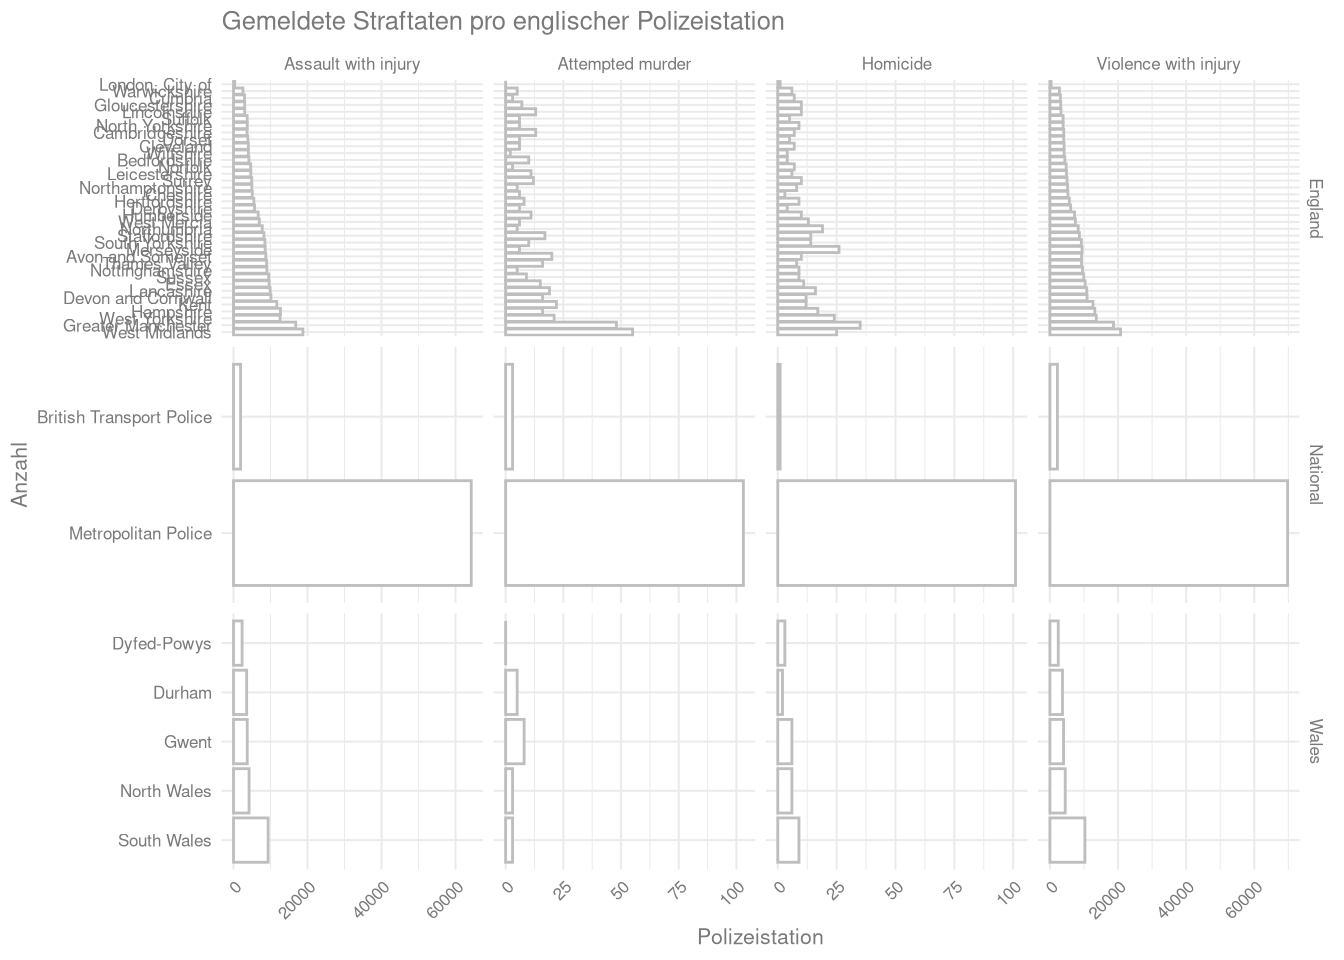
\includegraphics[width=333.333333333333pt]{R_Einfuehrung_111220_files/figure-latex/unnamed-chunk-110-1} \end{center}

\hypertarget{grafiken-exportieren}{%
\subsection{Grafiken exportieren}\label{grafiken-exportieren}}

Um die Auflösung zu verbessern können wir jetzt noch die Grafik mit anderen Seitenverhältnissen exportieren. Die \texttt{ggsave}-Funktion lässt uns einfach Grafiken in beliebigen Formaten exportieren.

\begin{Shaded}
\begin{Highlighting}[]
\FunctionTok{ggsave}\NormalTok{(}\AttributeTok{filename =} \StringTok{\textquotesingle{}imgs/police\_stations.png\textquotesingle{}}\NormalTok{,}
      \AttributeTok{width =} \DecValTok{50}\NormalTok{,}
      \AttributeTok{height =} \DecValTok{100}\NormalTok{,}
      \AttributeTok{units =} \StringTok{\textquotesingle{}cm\textquotesingle{}}\NormalTok{)}
\end{Highlighting}
\end{Shaded}

\begin{center}\includegraphics[width=.8\textwidth]{imgs/police_stations} \end{center}

\hypertarget{appendix}{%
\chapter{Appendix}\label{appendix}}

\hypertarget{nuxfctzliche-pakete}{%
\section{Nützliche Pakete}\label{nuxfctzliche-pakete}}

\hypertarget{rmarkdown}{%
\subsection{\texorpdfstring{\texttt{Rmarkdown}}{Rmarkdown}}\label{rmarkdown}}

Das Rmarkdown - Biotop ist das Ergebnis des Versuchs, die Hürde zur Kommunikation von Datenanalysen so gering wie möglich zu gestalten.

Mit der Hilfe der zugehörigen Pakete lassen sich in einer sehr einfachen Syntax schnell Code-Stücke aus inzwischen 6 Programmiersprachen mit Freitext und untereinander kombinieren und in einem Dokument verbinden. Dieses Dokument lässt sich dann dank Pandoc in einer Vielzahl von Formaten exportieren.

Um den Kern von Rmarkdown ist ein riesiger Apparat an Erweiterungen entstanden, die den Funktionsumfang zu einem sehr mächtigen Tool zur Dokumenterstellung anwachsen lassen. Dieses Skript ist zum Beispiel vollständig in Rmarkdown geschrieben.

Um ein Dokument zu erstellen muss man einfach auf ``neues Dokument'' \(\rightarrow\) R Markdown klicken und schon kann man anfangen.

Mit Paketen wie Bookdown, Shiny, Plotly und Blogdown lassen sich auch sehr attraktive interaktive Dokumente erstellen, die Beispielsweise direkt als Website nutzbar sind.

\hypertarget{wo-kann-ich-dazu-mehr-erfahren}{%
\subsubsection{Wo kann ich dazu mehr erfahren?}\label{wo-kann-ich-dazu-mehr-erfahren}}

\citet{grolemundMarkdownDefinitiveGuide} bieten \href{https://bookdown.org/yihui/rmarkdown/}{hier} ein frei zugängliches gitbook mit Antworten zu allen Fragen, die man zum Standard-markdown haben kann.

Yihui Xie, einer der Autoren, ist auch der Autor von \texttt{bookdown} und \texttt{blogdown}, seine Bücher dazu lassen sich auch empfehlen.

\hypertarget{skimr}{%
\subsection{\texorpdfstring{\texttt{skimr}}{skimr}}\label{skimr}}

\texttt{glimpse} und \texttt{summary} sind zwar ganz nett, da ein guter Überblick über die vorliegenden Daten aber entscheidend für den Erfolg jeder Datenanalyse ist, sind mehr dargestellte Informationen nur im Ausnahmefall unerwünscht.

Das \texttt{skimr}-Paket mit seiner \texttt{skim}-Funktion bietet fast alle Informationen, die man sich nur irgendwie wünschen kann.

\begin{Shaded}
\begin{Highlighting}[]
\NormalTok{skimr}\SpecialCharTok{::}\FunctionTok{skim}\NormalTok{(iris)}
\end{Highlighting}
\end{Shaded}

\hypertarget{ez}{%
\subsection{\texorpdfstring{\texttt{ez}}{ez}}\label{ez}}

Das \texttt{ez}-Paket stellt eine wesentliche Verbesserung der R-Syntax zur Auswertung faktorieller Experimente dar.

Als kleines Beispiel eine abhängige zweifaktorielle Varianzanalyse auf Basis des in \texttt{ez} mitgelieferten \texttt{ANT}-Datensatzes, der simulierte Ergebnisse des Attention Network Tests beinhalted.

\begin{Shaded}
\begin{Highlighting}[]
\FunctionTok{library}\NormalTok{(ez)}
\FunctionTok{data}\NormalTok{(ANT)}
\NormalTok{skimr}\SpecialCharTok{::}\FunctionTok{skim}\NormalTok{(ANT)}
\end{Highlighting}
\end{Shaded}

\hypertarget{klassische-vorgehensweise-in-base-r}{%
\subsubsection{klassische Vorgehensweise in base R}\label{klassische-vorgehensweise-in-base-r}}

\begin{Shaded}
\begin{Highlighting}[]
\NormalTok{anova }\OtherTok{\textless{}{-}} \FunctionTok{aov}\NormalTok{(rt }\SpecialCharTok{\textasciitilde{}}\NormalTok{ cue }\SpecialCharTok{*}\NormalTok{ flank }\SpecialCharTok{+} \FunctionTok{Error}\NormalTok{(subnum), }\AttributeTok{data =}\NormalTok{ ANT)}
\FunctionTok{summary}\NormalTok{(anova)}
\end{Highlighting}
\end{Shaded}

\begin{verbatim}
## 
## Error: subnum
##           Df Sum Sq Mean Sq F value Pr(>F)
## Residuals 19  85489    4499               
## 
## Error: Within
##             Df   Sum Sq Mean Sq  F value   Pr(>F)
## cue          3  5523668 1841223  698.350  < 2e-16
## flank        2  7871119 3935559 1492.703  < 2e-16
## cue:flank    6    79837   13306    5.047 3.58e-05
## Residuals 5729 15104697    2637                  
##              
## cue       ***
## flank     ***
## cue:flank ***
## Residuals    
## ---
## Signif. codes:  
## 0 '***' 0.001 '**' 0.01 '*' 0.05 '.' 0.1 ' ' 1
\end{verbatim}

\hypertarget{anova-mit-ez}{%
\subsubsection{\texorpdfstring{ANOVA mit \texttt{ez}}{ANOVA mit ez}}\label{anova-mit-ez}}

\begin{Shaded}
\begin{Highlighting}[]
\NormalTok{ANT }\SpecialCharTok{\%\textgreater{}\%} 
  \FunctionTok{ezANOVA}\NormalTok{(}
    \AttributeTok{dv =}\NormalTok{ rt,}
    \AttributeTok{wid =}\NormalTok{ subnum,}
    \AttributeTok{within =}\NormalTok{ .(cue,flank)}
\NormalTok{  )}
\end{Highlighting}
\end{Shaded}

\begin{verbatim}
## Warning: Collapsing data to cell means. *IF* the
## requested effects are a subset of the full design,
## you must use the "within_full" argument, else
## results may be inaccurate.
\end{verbatim}

\begin{verbatim}
## $ANOVA
##      Effect DFn DFd           F            p
## 2       cue   3  57  540.862407 7.988172e-42
## 3     flank   2  38 1066.037656 4.196305e-34
## 4 cue:flank   6 114    4.357093 5.356773e-04
##   p<.05        ges
## 2     * 0.87793881
## 3     * 0.91110583
## 4     * 0.09416982
## 
## $`Mauchly's Test for Sphericity`
##      Effect         W          p p<.05
## 2       cue 0.8431739 0.69690404      
## 3     flank 0.7999302 0.13411237      
## 4 cue:flank 0.1378186 0.03419366     *
## 
## $`Sphericity Corrections`
##      Effect       GGe        p[GG] p[GG]<.05
## 2       cue 0.9016877 6.126025e-38         *
## 3     flank 0.8332849 8.590878e-29         *
## 4 cue:flank 0.5956263 4.652864e-03         *
##         HFe        p[HF] p[HF]<.05
## 2 1.0657965 7.988172e-42         *
## 3 0.9037852 4.869100e-31         *
## 4 0.7506166 2.015937e-03         *
\end{verbatim}

\hypertarget{wo-kann-ich-dazu-mehr-erfahren-1}{%
\subsubsection{Wo kann ich dazu mehr erfahren?}\label{wo-kann-ich-dazu-mehr-erfahren-1}}

Die \href{https://www.rdocumentation.org/packages/ez/versions/4.4-0}{Dokumentation} von \texttt{ez} ist ziemlich gut.

\hypertarget{ggwordcloud}{%
\subsection{\texorpdfstring{\texttt{ggwordcloud}}{ggwordcloud}}\label{ggwordcloud}}

Für eher qualitative Darstellungen von Textdaten sind wordclouds manchmal ganz nett, das \texttt{ggwordcloud}-Paket kombiniert diesen Anspruch mit den Anpassungsmöglichkeiten von \texttt{ggplot2}.

Ein kleines Beispiel sind diese wordclouds, die auf einem Datensatz basieren, der die Berichterstattung über Corona in Schweden und Deutschland aus dem jeweils anderen Land abbildet:

\begin{Shaded}
\begin{Highlighting}[]
\FunctionTok{summary}\NormalTok{(stories)}
\end{Highlighting}
\end{Shaded}

\begin{verbatim}
##      word           translation       
##  Length:500         Length:500        
##  Class :character   Class :character  
##  Mode  :character   Mode  :character  
##                                       
##                                       
##                                       
##                                       
##    sentiment             n            country   
##  Min.   :-5.0000   Min.   :  440   Germany:250  
##  1st Qu.:-1.5000   1st Qu.:  698   Sweden :250  
##  Median : 1.0000   Median : 1656                
##  Mean   : 0.4639   Mean   : 1989                
##  3rd Qu.: 2.0000   3rd Qu.: 2405                
##  Max.   : 5.0000   Max.   :15223                
##  NA's   :445
\end{verbatim}

Diesen Datensatz wollen wir jetzt als eine wordcloud pro Nation darstellen:

\begin{Shaded}
\begin{Highlighting}[]
\FunctionTok{library}\NormalTok{(ggwordcloud)}
\NormalTok{stories }\SpecialCharTok{\%\textgreater{}\%} 
  \FunctionTok{ggplot}\NormalTok{(}\FunctionTok{aes}\NormalTok{(}\AttributeTok{size =}\NormalTok{ n, }
             \AttributeTok{label =}\NormalTok{ word,}
             \AttributeTok{alpha =}\NormalTok{ n)) }\SpecialCharTok{+}
  \FunctionTok{geom\_text\_wordcloud}\NormalTok{(}\AttributeTok{rm\_outside =}\NormalTok{ T,}
                      \AttributeTok{color =} \StringTok{\textquotesingle{}darkblue\textquotesingle{}}\NormalTok{) }\SpecialCharTok{+}
  \FunctionTok{facet\_grid}\NormalTok{(}\SpecialCharTok{\textasciitilde{}}\NormalTok{country) }\SpecialCharTok{+}
  \FunctionTok{theme\_minimal}\NormalTok{()}
\end{Highlighting}
\end{Shaded}

\begin{flushleft}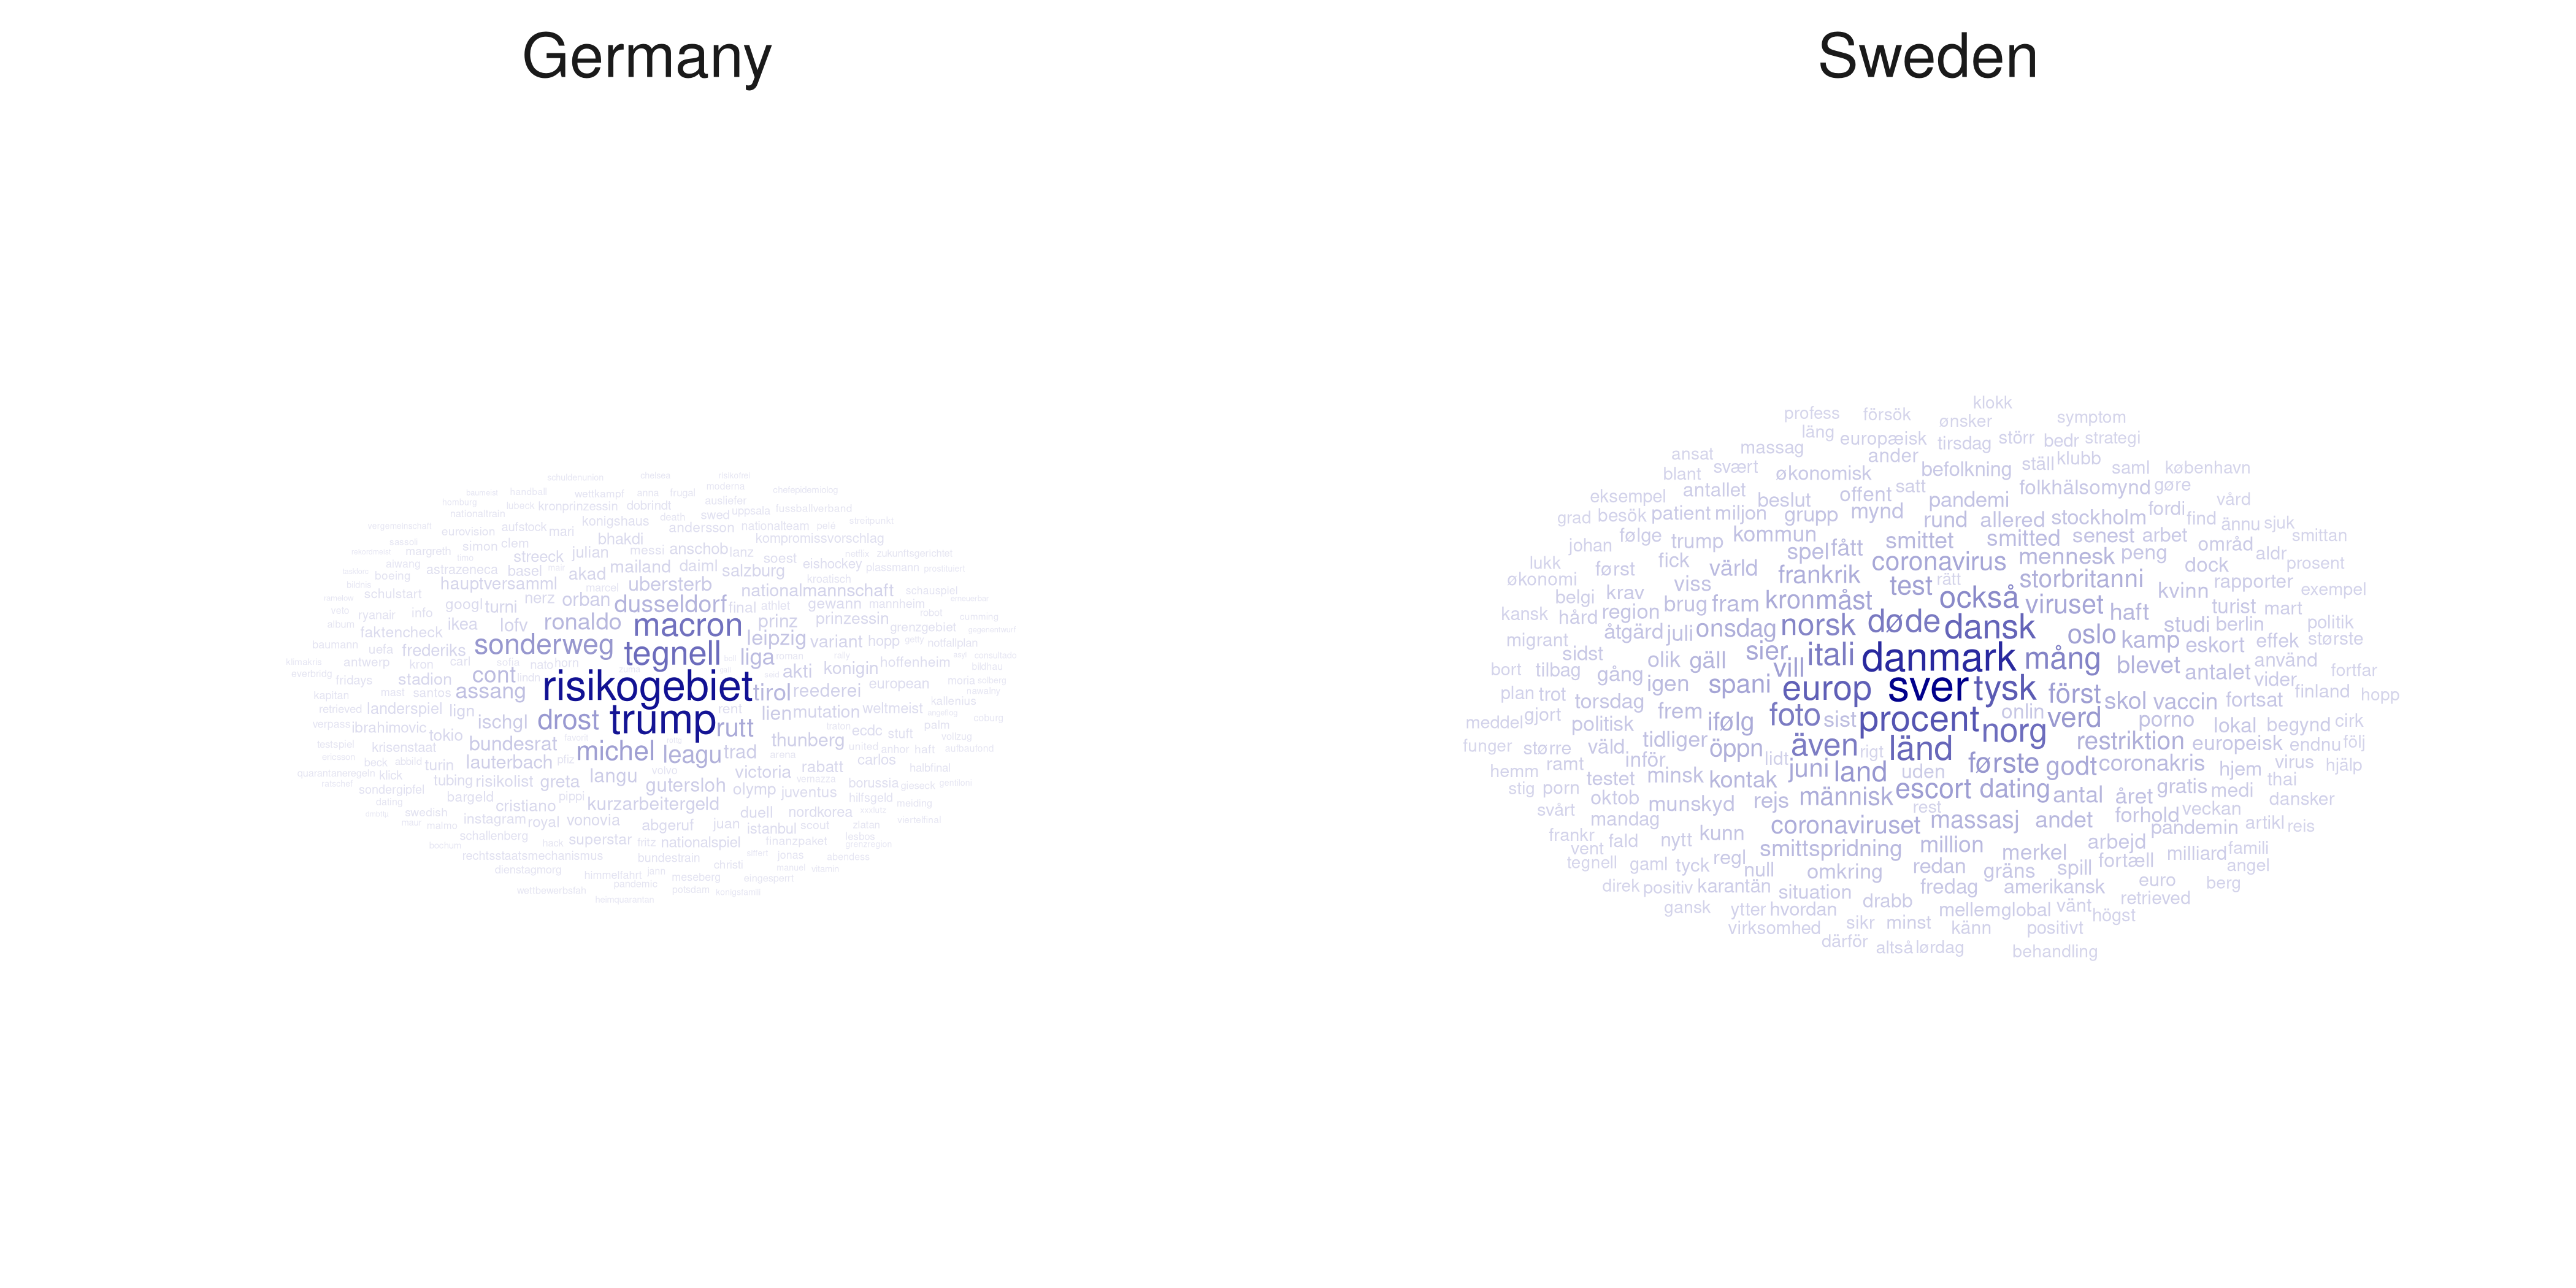
\includegraphics[width=333.333333333333pt]{imgs/wc} \end{flushleft}

\hypertarget{wo-kann-ich-dazu-mehr-erfahren-2}{%
\subsubsection{Wo kann ich dazu mehr erfahren?}\label{wo-kann-ich-dazu-mehr-erfahren-2}}

Die Vignette von ggwordcloud bietet ein paar schöne Beispiele, an denen man sich gut entlang hangeln kann.

Zum Öffnen nach dem Laden des Pakets einfach so aufrufen:

\begin{Shaded}
\begin{Highlighting}[]
\FunctionTok{vignette}\NormalTok{(}\StringTok{\textquotesingle{}ggwordcloud\textquotesingle{}}\NormalTok{)}
\end{Highlighting}
\end{Shaded}

\hypertarget{plotly}{%
\subsection{\texorpdfstring{\texttt{plotly}}{plotly}}\label{plotly}}

Plotly ist ein nicht nur in R implementiertes Software-Paket, dass es mit wenigen Schritten ermöglicht, interaktive Grafiken zu erstellen.

Wir können das, was wir für ggplot gelernt haben, einfach für plotly anwenden:

\begin{Shaded}
\begin{Highlighting}[]
\FunctionTok{library}\NormalTok{(plotly)}
\end{Highlighting}
\end{Shaded}

\begin{verbatim}
## 
## Attaching package: 'plotly'
\end{verbatim}

\begin{verbatim}
## The following object is masked from 'package:ggplot2':
## 
##     last_plot
\end{verbatim}

\begin{verbatim}
## The following object is masked from 'package:stats':
## 
##     filter
\end{verbatim}

\begin{verbatim}
## The following object is masked from 'package:graphics':
## 
##     layout
\end{verbatim}

\begin{Shaded}
\begin{Highlighting}[]
\NormalTok{p }\OtherTok{\textless{}{-}}\NormalTok{ iris }\SpecialCharTok{\%\textgreater{}\%} 
  \FunctionTok{ggplot}\NormalTok{(}\FunctionTok{aes}\NormalTok{(}\AttributeTok{x =}\NormalTok{ Sepal.Width,}
             \AttributeTok{y =}\NormalTok{ Sepal.Length,}
             \AttributeTok{color =}\NormalTok{ Species)) }\SpecialCharTok{+}
  \FunctionTok{geom\_point}\NormalTok{() }\SpecialCharTok{+}
  \FunctionTok{theme\_light}\NormalTok{() }\SpecialCharTok{+}
  \FunctionTok{theme}\NormalTok{(}\AttributeTok{legend.position =} \StringTok{\textquotesingle{}none\textquotesingle{}}\NormalTok{)}

\NormalTok{p}
\end{Highlighting}
\end{Shaded}

\begin{center}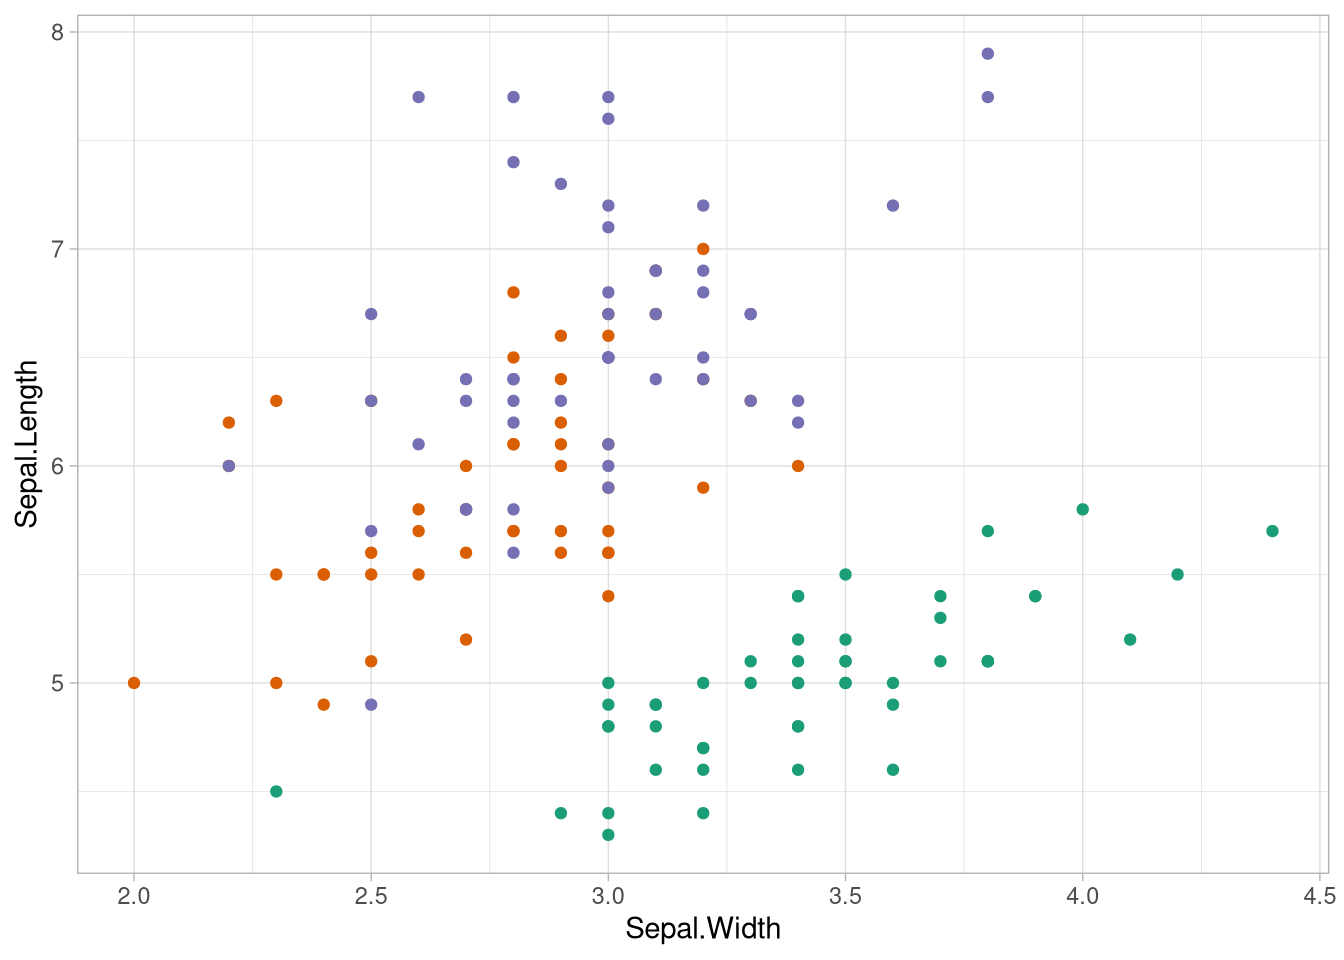
\includegraphics[width=333.333333333333pt]{R_Einfuehrung_111220_files/figure-latex/unnamed-chunk-121-1} \end{center}

Um den Graphen interaktiv zu gestalten reicht es, ihn an \texttt{ggplotly} zu übergeben:

\begin{Shaded}
\begin{Highlighting}[]
\FunctionTok{ggplotly}\NormalTok{(p)}
\end{Highlighting}
\end{Shaded}

\begin{verbatim}
## PhantomJS not found. You can install it with webshot::install_phantomjs(). If it is installed, please make sure the phantomjs executable can be found via the PATH variable.
\end{verbatim}

\hypertarget{htmlwidget-e4ceb87f7068dc58768f}{}

\hypertarget{wo-kann-ich-dazu-mehr-erfahren-3}{%
\subsubsection{Wo kann ich dazu mehr erfahren?}\label{wo-kann-ich-dazu-mehr-erfahren-3}}

Wenn komplexere Grafiken gewünscht sind, ist die \href{https://plotly.com/r/}{plotly-Website} eine gute Ressource um anzufangen.

Für die meisten Anwendungsfälle reicht es aber aus, den Graphen mit ggplot zu erstellen und den automatischen Port zu verwenden.

\hypertarget{lavaan}{%
\subsection{\texorpdfstring{\texttt{lavaan}}{lavaan}}\label{lavaan}}

Das \texttt{lavaan}-Projekt und das zugehörige Paket ist in den Worten der Entwickler:

\begin{quote}
The lavaan package is developed to provide useRs, researchers and teachers a free open-source, but commercial-quality package for latent variable modeling. \href{https://lavaan.ugent.be/index.html}{Von der lavaan-Homepage}
\end{quote}

Und kann inzwischen genutzt werden um so gut wie jedes Modell zur Analyse latenter Variablen aufzustellen, zu schätzen und zu testen.

Das Paket ist so umfrangreich, dass wir es hier nur in anekdotischer Art besprechen können, wir gehen aber ein Beispiel für ein SEM durch.

Wir versuchen die Auswertung aus \citet{pishghadamIntelligenceMetacognitionPredictors2013} mit lavaan nachzuvollziehen. Die Autoren berichten dankenswerterweise Korrelationsmatrizen und Streuungen, daraus können wir uns einfach die folgende Kovarianzmatrix bauen:

\textbackslash begin\{table\}

\textbackslash caption\{\label{tab:unnamed-chunk-123}kc steht für \emph{knowledge of cognition}, rc für \emph{regulation of cognition} und fla\_test für das Ergebnis eines \emph{foreign language achievement}\}
\centering

\begin{tabular}[t]{lrrrrrrr}
\toprule
  & IQ1 & IQ2 & Total Intelligence & kc & rc & total\_metacognition & fla\_test\\
\midrule
IQ1 & 7.95 & 3.62 & 8.79 & 4.60 & 5.28 & 9.96 & 3.45\\
IQ2 & 3.62 & 10.82 & 11.10 & 8.26 & 7.70 & 16.27 & 4.22\\
Total Intelligence & 8.79 & 11.10 & 26.11 & 12.83 & 13.15 & 27.07 & 7.75\\
kc & 4.60 & 8.26 & 12.83 & 157.50 & 185.01 & 261.53 & 31.46\\
rc & 5.28 & 7.70 & 13.15 & 185.01 & 547.56 & 512.42 & 53.20\\
\addlinespace
total\_metacognition & 9.96 & 16.27 & 27.07 & 261.53 & 512.42 & 1247.50 & 84.43\\
fla\_test & 3.45 & 4.22 & 7.75 & 31.46 & 53.20 & 84.43 & 33.99\\
\bottomrule
\end{tabular}

\textbackslash end\{table\}

Als nächsten Schritt laden wir \texttt{lavaan} und formulieren das Modell nach, das die Autoren aufgestellt haben:

\begin{Shaded}
\begin{Highlighting}[]
\FunctionTok{library}\NormalTok{(lavaan)}
\end{Highlighting}
\end{Shaded}

\begin{verbatim}
## This is lavaan 0.6-7
\end{verbatim}

\begin{verbatim}
## lavaan is BETA software! Please report any bugs.
\end{verbatim}

\begin{Shaded}
\begin{Highlighting}[]
\NormalTok{my\_model }\OtherTok{\textless{}{-}} \StringTok{\textquotesingle{}}
\StringTok{\#\# Definiton latenter Variablen:}
\StringTok{Intelligence =\textasciitilde{} IQ1 + IQ2}
\StringTok{Metacognition =\textasciitilde{} kc + rc}
\StringTok{fla =\textasciitilde{} fla\_test}

\StringTok{\# Korrelationen}
\StringTok{Intelligence \textasciitilde{}\textasciitilde{} Metacognition}
\StringTok{fla \textasciitilde{}\textasciitilde{} Intelligence }
\StringTok{fla \textasciitilde{}\textasciitilde{} Metacognition}
\StringTok{\textquotesingle{}}
\end{Highlighting}
\end{Shaded}

Das Gesamtmodell, die Stichprobengröße von 143 und die Kovarianzmatrix übergeben wir jetzt an \texttt{sem}:

\begin{Shaded}
\begin{Highlighting}[]
\NormalTok{sem\_example }\OtherTok{\textless{}{-}} \FunctionTok{sem}\NormalTok{(}
\NormalTok{  my\_model,}
    \AttributeTok{sample.cov =}\NormalTok{ cov\_mat,}
    \AttributeTok{sample.nobs =} \DecValTok{143}\NormalTok{)}

\FunctionTok{summary}\NormalTok{(sem\_example, }\AttributeTok{standardized =} \ConstantTok{TRUE}\NormalTok{)}
\end{Highlighting}
\end{Shaded}

\begin{verbatim}
## lavaan 0.6-7 ended normally after 142 iterations
## 
##   Estimator                                         ML
##   Optimization method                           NLMINB
##   Number of free parameters                         12
##                                                       
##   Number of observations                           143
##                                                       
## Model Test User Model:
##                                                       
##   Test statistic                                 1.790
##   Degrees of freedom                                 3
##   P-value (Chi-square)                           0.617
## 
## Parameter Estimates:
## 
##   Standard errors                             Standard
##   Information                                 Expected
##   Information saturated (h1) model          Structured
## 
## Latent Variables:
##                    Estimate  Std.Err  z-value
##   Intelligence =~                            
##     IQ1               1.000                  
##     IQ2               1.313    0.548    2.399
##   Metacognition =~                           
##     kc                1.000                  
##     rc                1.641    0.289    5.669
##   fla =~                                     
##     fla_test          1.000                  
##   P(>|z|)   Std.lv  Std.all
##                            
##              1.654    0.589
##     0.016    2.172    0.663
##                            
##             10.581    0.846
##     0.000   17.363    0.745
##                            
##              5.810    1.000
## 
## Covariances:
##                    Estimate  Std.Err  z-value
##   Intelligence ~~                            
##     Metacognition     4.852    2.545    1.907
##     fla               3.287    1.371    2.397
##   Metacognition ~~                           
##     fla              31.557    6.618    4.768
##   P(>|z|)   Std.lv  Std.all
##                            
##     0.057    0.277    0.277
##     0.017    0.342    0.342
##                            
##     0.000    0.513    0.513
## 
## Variances:
##                    Estimate  Std.Err  z-value
##    .IQ1               5.161    1.278    4.037
##    .IQ2               6.030    2.064    2.921
##    .kc               44.446   18.448    2.409
##    .rc              242.250   55.573    4.359
##    .fla_test          0.000                  
##     Intelligence      2.736    1.327    2.061
##     Metacognition   111.955   25.044    4.470
##     fla              33.751    3.992    8.456
##   P(>|z|)   Std.lv  Std.all
##     0.000    5.161    0.654
##     0.003    6.030    0.561
##     0.016   44.446    0.284
##     0.000  242.250    0.446
##              0.000    0.000
##     0.039    1.000    1.000
##     0.000    1.000    1.000
##     0.000    1.000    1.000
\end{verbatim}

Mit \texttt{fitmeasures(sem\_example)} können wir uns die gängigsten fit-Indizes und noch ein paar mehr ausgeben lassen:

\begin{Shaded}
\begin{Highlighting}[]
\FunctionTok{fitmeasures}\NormalTok{(sem\_example)}
\end{Highlighting}
\end{Shaded}

\begin{verbatim}
##                npar                fmin 
##              12.000               0.006 
##               chisq                  df 
##               1.790               3.000 
##              pvalue      baseline.chisq 
##               0.617             141.806 
##         baseline.df     baseline.pvalue 
##              10.000               0.000 
##                 cfi                 tli 
##               1.000               1.031 
##                nnfi                 rfi 
##               1.031               0.958 
##                 nfi                pnfi 
##               0.987               0.296 
##                 ifi                 rni 
##               1.009               1.009 
##                logl   unrestricted.logl 
##           -2325.277           -2324.382 
##                 aic                 bic 
##            4674.555            4710.109 
##              ntotal                bic2 
##             143.000            4672.139 
##               rmsea      rmsea.ci.lower 
##               0.000               0.000 
##      rmsea.ci.upper        rmsea.pvalue 
##               0.116               0.735 
##                 rmr          rmr_nomean 
##               1.154               1.154 
##                srmr        srmr_bentler 
##               0.019               0.019 
## srmr_bentler_nomean                crmr 
##               0.019               0.023 
##         crmr_nomean          srmr_mplus 
##               0.023               0.019 
##   srmr_mplus_nomean               cn_05 
##               0.019             625.194 
##               cn_01                 gfi 
##             907.160               0.995 
##                agfi                pgfi 
##               0.975               0.199 
##                 mfi                ecvi 
##               1.004               0.180
\end{verbatim}

Und mit dem semPlot-Paket lässt sich das Modell auch darstellen:

\begin{Shaded}
\begin{Highlighting}[]
\NormalTok{semPlot}\SpecialCharTok{::}\FunctionTok{semPaths}\NormalTok{(sem\_example, }
                  \AttributeTok{what =} \StringTok{\textquotesingle{}path\textquotesingle{}}\NormalTok{, }
                  \AttributeTok{whatLabels =} \StringTok{\textquotesingle{}std\textquotesingle{}}\NormalTok{, }
                  \AttributeTok{layout =} \StringTok{\textquotesingle{}spring\textquotesingle{}}\NormalTok{, }
                  \AttributeTok{residuals =}\NormalTok{ F)}
\end{Highlighting}
\end{Shaded}

\begin{verbatim}
## Registered S3 methods overwritten by 'huge':
##   method    from   
##   plot.sim  BDgraph
##   print.sim BDgraph
\end{verbatim}

\begin{center}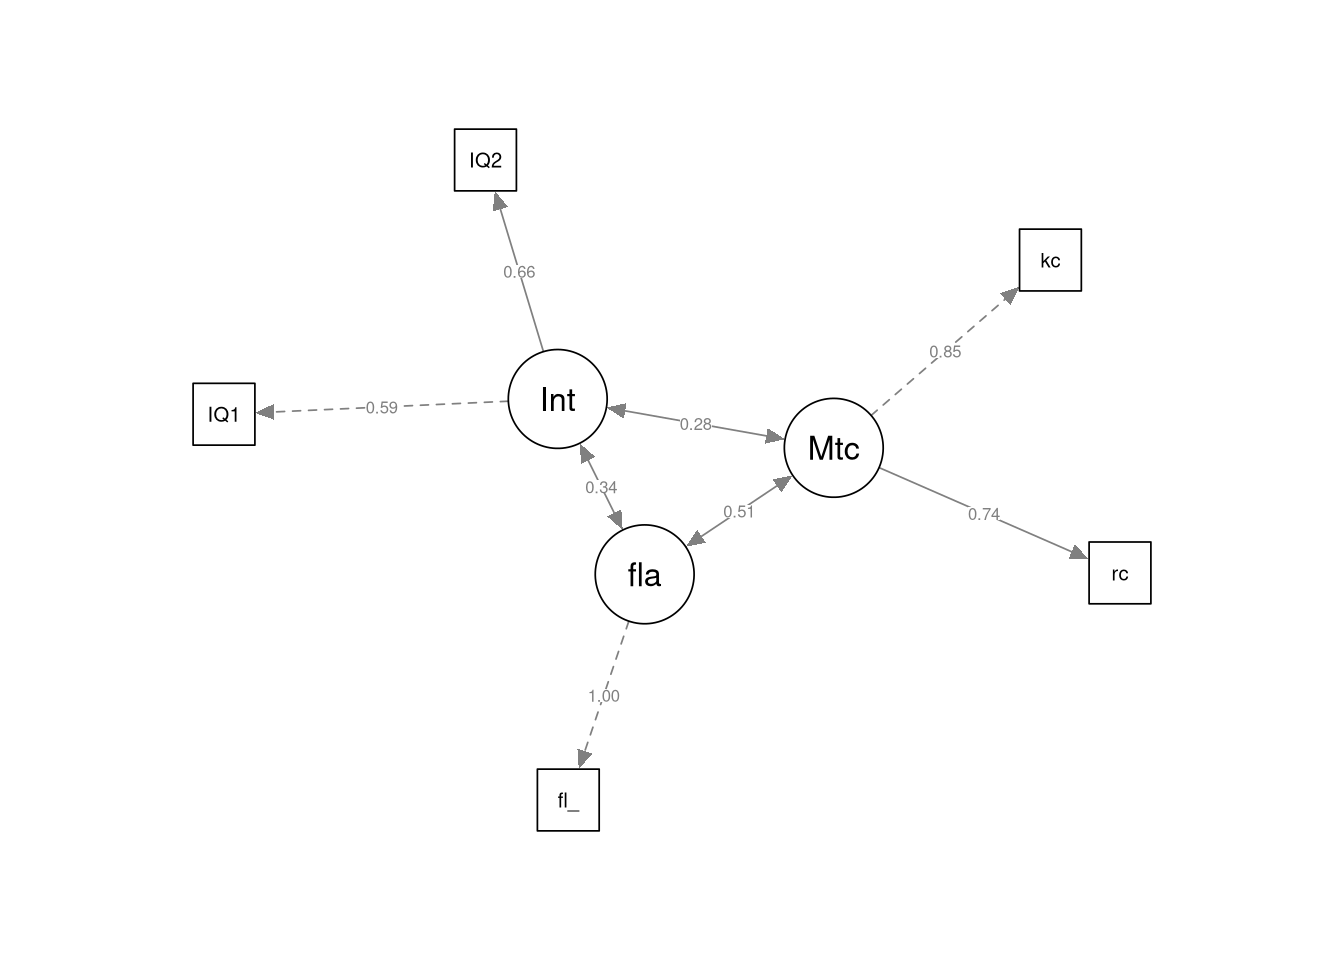
\includegraphics[width=333.333333333333pt]{R_Einfuehrung_111220_files/figure-latex/unnamed-chunk-127-1} \end{center}

\hypertarget{wo-kann-ich-dazu-mehr-erfahren-4}{%
\subsubsection{Wo kann ich dazu mehr erfahren?}\label{wo-kann-ich-dazu-mehr-erfahren-4}}

Zum Lernen von \texttt{lavaan} stellen die Autoren \href{https://lavaan.ugent.be/resources/teaching.html}{hier} einen großen Pool an Materialien zur Verfügung.

Für das \texttt{semPlot}-Paket sind die Ressourcen leider nicht so gut, die Dokumentation der \texttt{semPaths}-Funktion ist aber ziemlich gut, zu finden nach dem Laden des Pakets mit \texttt{?semPaths}.

\hypertarget{andere-ressourcen}{%
\section{Andere Ressourcen}\label{andere-ressourcen}}

\hypertarget{cheatsheets}{%
\subsubsection{Cheatsheets}\label{cheatsheets}}

RStudio stellt eine ganze Reihe von hilfreichen Spickzetteln zu Verfügung, die den workflow effizienter macen indem sie die wichtigsten Funktionen auf einen Blick übersichtlich machen. Die Cheatsheets finden sich \href{https://rstudio.com/resources/cheatsheets/}{hier}

Exemplarisch für die bisher besprochenen Pakete sind die folgenden Cheatsheets zu empfehlen:

\begin{itemize}
\item
  \href{https://github.com/rstudio/cheatsheets/raw/master/factors.pdf}{forcats}
\item
  \href{https://github.com/rstudio/cheatsheets/raw/master/data-import.pdf}{Daten importieren}
\item
  \href{https://github.com/rstudio/cheatsheets/raw/master/data-transformation.pdf}{dplyr}
\item
  \href{https://github.com/rstudio/cheatsheets/raw/master/rstudio-ide.pdf}{die RStudio-IDE}
\item
  \href{https://github.com/rstudio/cheatsheets/raw/master/data-visualization-2.1.pdf}{ggplot2}
\end{itemize}

\hypertarget{buxfccher}{%
\subsubsection{Bücher}\label{buxfccher}}

Wenn man tiefer in tidy data analysis mit R einsteigen möchte kommt man an den Büchern von Hadley Wickham (Autor von ggplot2 und Chief Scientist bei RStudio) nicht vorbei. Die wichtigsten sind frei online zugänglich, dabei sind besonders die folgenden zu empfehlen:

\begin{itemize}
\item
  \citep[\emph{R for Data Science}][]{grolemundDataScience}(\url{https://r4ds.had.co.nz/}) für die Grundlagen und
\item
  \citep[\emph{Advanced R}][]{wickhamAdvanced2019}(\url{https://adv-r.hadley.nz/}) für fortgeschrittenere Themen
\end{itemize}

  \bibliography{book.bib}

\end{document}
